\documentclass[a4paper,11pt]{article}

\usepackage{fullpage}
\usepackage{fancyvrb}
\usepackage[table]{xcolor}
\usepackage{amsmath}
\usepackage{amssymb}
\usepackage{hyperref}
% See https://tex.stackexchange.com/questions/559742/make-hyperref-links-only-show-up-if-theyre-external-links
\makeatletter
% first six lines of nohyperref.sty
% keep anchors
%\let\hyper@@anchor\@gobble
\def\hyper@link#1#2#3{#3}%
%\let\hyper@anchorstart\@gobble
%\let\hyper@anchorend\@empty
\let\hyper@linkstart\@gobbletwo
\let\hyper@linkend\@empty
\makeatother
\usepackage[pass]{geometry}
\usepackage{pdflscape}
\usepackage{booktabs}
\usepackage{musicography}
\usepackage{caption}
\usepackage{subcaption}
\usepackage{appendix}
\usepackage{tikz}
\usepackage{rotating}
\usepackage{booktabs}

\usepackage{biblatex}
\addbibresource{wilson_keyboard_mapping.bib}

\usepackage{nicematrix}
\NiceMatrixOptions{
code-for-first-row = \scriptstyle \color{gray} ,
code-for-last-row = \scriptstyle \color{gray} ,
code-for-first-col = \scriptstyle \color{gray} ,
}

\newcommand\myslash{\rotatebox[origin=c]{-30}{$\vert$}}

\newcommand\red{\mathbin{\mathrm{red}}}

\newcommand\matspace{\:}

\newcommand\intervalsep{\,--\,}

\setlength{\parskip}{\baselineskip}
\setlength{\parindent}{0pt}

\begin{document}
\title{
\vspace{-2.5cm}
Another look at Wilson's keyboard mapping system
\vspace{-0.5cm}
}
\author{\vspace{-0.5cm}Naren Ratan}
\date{\vspace{-0.5cm}23rd March 2026\vspace{-1cm}}
\maketitle
\section{Introduction}
A portion of Erv Wilson's keyboard mapping system can be expressed in a few
equations. Personally I find that the equations help to apply and understand
the system. This article presents the equations and gives examples of their
use. Section \ref{context} gives some context. Section \ref{bases} defines
lattice bases. Section \ref{sec:scale-degree-mapping} presents mapping based on
scale degree. Section \ref{harmonic_template_mapping} presents mapping using
harmonic templates, including an optimization problem for finding nice keyboard
mappings. Section \ref{chain_position} discusses chain position and keyboard
coordinates. Section \ref{sec:notation} describes musical notations based on
keyboard mappings. Section \ref{playing} discusses playing the keyboard
mappings on a Launchpad MIDI controller (the fun part!).

\section{Context}
\label{context}
By keyboard mapping I mean laying out a scale on a two-dimensional keyboard
\cite{narushima2017microtonality}. For example, Figure \ref{fig:partch-example}
shows one possible mapping for Harry Partch's 43-tone scale
\cite{partch1979genesis}. The general question is, given a particular scale,
how can we go about mapping it onto a keyboard?  Of course we could just place
the notes at random; the problem is to find mappings which are easy to play
and, perhaps, give some insight into the structure of the scale.

\begin{figure}[h]
\vspace{0.35cm}
\begin{center}
\input{xen03-secor-partch.tex}
\end{center}
\caption{One possible keyboard mapping for Partch's 43-tone scale.}
\label{fig:partch-example}
\end{figure}

\section{Lattice bases}
\label{bases}
The keys on the keyboard are labeled by pairs of integers $(x, y)$, their $x$
and $y$ coordinates. The set of all these integer pairs is called a lattice
\cite{cassels1959geometry, schrijver1998theory}.

Wilson's keyboard mappings often place 3/2 at $(a, b)$ and 2/1 at $(c, d)$ such
that $ad - bc = -1$. This relation is fundamental in Wilson's keyboard mapping
theory \cite{wilsondiophantine}. To understand it, we can use the concept of a
lattice basis.

For two lattice points $(a, b)$ and $(c, d)$, if we can write any lattice point
$(x, y)$ as
\begin{align}
\begin{bmatrix}
    x \\
    y \\
\end{bmatrix}
    &=
    p
\begin{bmatrix}
    a \\
    b \\
\end{bmatrix}
    +
    q
\begin{bmatrix}
    c \\
    d \\
\end{bmatrix}
\end{align}
with integer $p$ and $q$, we say $(a, b)$ and $(c, d)$ form a basis for the
lattice.

The one fact we need about lattices is that $(a, b)$ and $(c, d)$ form a basis
if and only if $ad - bc = \pm 1$. So a lattice basis is quite a special thing.

We'll see exactly how lattice bases come up throughout Wilson's keyboard
mapping theory. For now I'll just note that Wilson's Gral spectrum
\cite{wilsongralspectrum} is effectively a gallery of lattice bases, and that a
basis allows us to define Wilson's chain position, which appears to be
fundamental in his thinking.

\section{Scale degree mapping}
\label{sec:scale-degree-mapping}
One way to map a scale is to always go up the same number of scale degrees when
going one key along a row or up a column. So a mapping of this sort is
determined by two numbers, the $x$ and $y$ step sizes --- call them $s$ and
$t$. For example, we could map Partch's scale by taking the $x$ step as $s = 2$
and the $y$ step as $t = 7$ to give the mapping in Figure \ref{fig:partch2-7}.
Here each key is labeled with the ratio in the middle, cents at the bottom,
and scale degree at the top followed by a dot (e.g. $2.$). You can see that the
scale degree always goes up by 2 going one key along a row, and that it goes up
by 7 going one key up a column. The mapping in Figure \ref{fig:partch2-7} works
well for playing Partch's scale on a Launchpad (see Section \ref{playing}).

\begin{figure}
\begin{center}
$\begin{NiceArray}[first-col, last-row, columns-width=1.1cm]{|c|c|c|c|c|c|c|c|}
\hline
 &    \scriptstyle 36.
 &    \scriptstyle 38.
 &    \scriptstyle 40.
 &    \scriptstyle 42.
 &    \scriptstyle 44.
 &    \scriptstyle 46.
 &    \scriptstyle 48.
 &    \scriptstyle 50.
\\
6 &    9/5
 &    11/6
 &    40/21
 &    160/81
 &    
 &    
 &    
 &    
\\
 &    \scriptstyle 1018
 &    \scriptstyle 1049
 &    \scriptstyle 1116
 &    \scriptstyle 1178
 &    \scriptstyle 
 &    \scriptstyle 
 &    \scriptstyle 
 &    \scriptstyle 
\\
\hline
 &    \scriptstyle 29.
 &    \scriptstyle 31.
 &    \scriptstyle 33.
 &    \scriptstyle 35.
 &    \scriptstyle 37.
 &    \scriptstyle 39.
 &    \scriptstyle 41.
 &    \scriptstyle 43.
\\
5 &    8/5
 &    5/3
 &    12/7
 &    16/9
 &    20/11
 &    15/8
 &    64/33
 &    2/1
\\
 &    \scriptstyle 814
 &    \scriptstyle 884
 &    \scriptstyle 933
 &    \scriptstyle 996
 &    \scriptstyle 1035
 &    \scriptstyle 1088
 &    \scriptstyle 1147
 &    \scriptstyle 1200
\\
\hline
 &    \scriptstyle 22.
 &    \scriptstyle 24.
 &    \scriptstyle 26.
 &    \scriptstyle 28.
 &    \scriptstyle 30.
 &    \scriptstyle 32.
 &    \scriptstyle 34.
 &    \scriptstyle 36.
\\
4 &    10/7
 &    40/27
 &    32/21
 &    11/7
 &    18/11
 &    27/16
 &    7/4
 &    9/5
\\
 &    \scriptstyle 618
 &    \scriptstyle 680
 &    \scriptstyle 729
 &    \scriptstyle 782
 &    \scriptstyle 853
 &    \scriptstyle 906
 &    \scriptstyle 969
 &    \scriptstyle 1018
\\
\hline
 &    \scriptstyle 15.
 &    \scriptstyle 17.
 &    \scriptstyle 19.
 &    \scriptstyle 21.
 &    \scriptstyle 23.
 &    \scriptstyle 25.
 &    \scriptstyle 27.
 &    \scriptstyle 29.
\\
3 &    14/11
 &    21/16
 &    27/20
 &    7/5
 &    16/11
 &    3/2
 &    14/9
 &    8/5
\\
 &    \scriptstyle 418
 &    \scriptstyle 471
 &    \scriptstyle 520
 &    \scriptstyle 582
 &    \scriptstyle 649
 &    \scriptstyle 702
 &    \scriptstyle 765
 &    \scriptstyle 814
\\
\hline
 &    \scriptstyle 8.
 &    \scriptstyle 10.
 &    \scriptstyle 12.
 &    \scriptstyle 14.
 &    \scriptstyle 16.
 &    \scriptstyle 18.
 &    \scriptstyle 20.
 &    \scriptstyle 22.
\\
2 &    9/8
 &    7/6
 &    6/5
 &    5/4
 &    9/7
 &    4/3
 &    11/8
 &    10/7
\\
 &    \scriptstyle 204
 &    \scriptstyle 267
 &    \scriptstyle 316
 &    \scriptstyle 386
 &    \scriptstyle 435
 &    \scriptstyle 498
 &    \scriptstyle 551
 &    \scriptstyle 618
\\
\hline
 &    \scriptstyle 1.
 &    \scriptstyle 3.
 &    \scriptstyle 5.
 &    \scriptstyle 7.
 &    \scriptstyle 9.
 &    \scriptstyle 11.
 &    \scriptstyle 13.
 &    \scriptstyle 15.
\\
1 &    81/80
 &    21/20
 &    12/11
 &    10/9
 &    8/7
 &    32/27
 &    11/9
 &    14/11
\\
 &    \scriptstyle 22
 &    \scriptstyle 84
 &    \scriptstyle 151
 &    \scriptstyle 182
 &    \scriptstyle 231
 &    \scriptstyle 294
 &    \scriptstyle 347
 &    \scriptstyle 418
\\
\hline
 &    \scriptstyle -6.
 &    \scriptstyle -4.
 &    \scriptstyle -2.
 &    \scriptstyle 0.
 &    \scriptstyle 2.
 &    \scriptstyle 4.
 &    \scriptstyle 6.
 &    \scriptstyle 8.
\\
0 &    
 &    
 &    
 &    1/1
 &    33/32
 &    16/15
 &    11/10
 &    9/8
\\
 &    \scriptstyle 
 &    \scriptstyle 
 &    \scriptstyle 
 &    \scriptstyle 0
 &    \scriptstyle 53
 &    \scriptstyle 112
 &    \scriptstyle 165
 &    \scriptstyle 204
\\
\hline
& -3 & -2 & -1 & 0 & 1 & 2 & 3 & 4
\end{NiceArray}$
\end{center}

\caption{Partch's scale mapped by scale degree with $x$ step size 2 and $y$
step size 7.}
\label{fig:partch2-7}
\end{figure}

\clearpage
\subsection{The Gral method}
When mapping by scale degree we can pick whichever step sizes $s$ and $t$ we
like. But if we choose scale degrees $m$ and $n$ which we want to form a basis
on the keyboard, we can solve for $s$ and $t$. Say the basis is $(a, b)$, $(c,
d)$. The conditions that scale degree $m$ is mapped to $(a, b)$ and scale
degree $n$ is mapped to $(c, d)$ give two equations
\begin{align}
    a s + b t &= m \\
    c s + d t &= n \label{eq:step-sizes}
\end{align}
which we can solve for the step sizes $s$ and $t$ to give
\begin{align}
    s &= \frac{dm-bn}{\Delta} \\
    t &= \frac{-cm + an}{\Delta},
\end{align}
where $\Delta = ad - bc$, and $\Delta = \pm 1$ since $(a, b)$, $(c, d)$ form a
basis.

Now say we want the step sizes to be positive, so scale degree (and so pitch)
increases along a row and up a column. This gives the conditions
\begin{align}
    \frac{ dm - bn}{\Delta} & > 0 \label{eq:positive-1}\\
    \frac{-cm + an}{\Delta} & > 0.\label{eq:positive-2}
\end{align}
If $\Delta = -1$, $c > 0$, and $d > 0$, these conditions are equivalent to
\begin{align}
    \frac{a}{c} < \frac{m}{n} < \frac{b}{d}\ .
\label{eq:positive-special}
\end{align}
So if we want positive step sizes then our choice of basis is restricted.
Wilson's Gral method \cite{wilsongralkeyboard, wilsongralspectrum} finds all
bases with $\Delta = -1$ which satisfy $a/c < m/n < b/d$ and which also have
non-negative coordinates ($a, b, c, d \geq 0$).

The Gral method is a binary search for the fraction $m/n$, starting with the
interval $[0/1, 1/0]$ and `bisecting' each interval $[a/c, b/d]$ with the
mediant $(a+b)/(c+d)$. For a wonderful discussion of the algorithm and its
relation to Farey series and the Stern-Brocot tree see
\cite[121]{knuth1994concrete}. It turns out that each interval $[a/c, b/d]$ we
encounter in the search has $ad - bc = -1$, so $(a, b)$, $(c, d)$ form a basis,
and $a/c < m/n < b/d$ since $m/n$ is in each search interval.

\clearpage
\begin{table}
\centering
\begin{tabular}{rr@{\hspace{1cm}}r@{\hspace{1cm}}rr@{\hspace{1cm}}rr@{\hspace{1cm}}rr}
\toprule
Left    &   Right   &   Mediant &   $a$  &  $b$  &  $c$  &  $d$  &  $s$  &  $t$  \\
\midrule
$0/1$ & $1/0$ & $1/1$ & $0$ & $1$ & $1$ & $0$ & $43$ & $25$ \\
    & $1/1$ & $1/2$ & $0$ & $1$ & $1$ & $1$ & $18$ & $25$ \\
$1/2$ &     & $2/3$ & $1$ & $1$ & $2$ & $1$ & $18$ & $7$ \\
    & $2/3$ & $3/5$ & $1$ & $2$ & $2$ & $3$ & $11$ & $7$ \\
    & $3/5$ & $4/7$ & $1$ & $3$ & $2$ & $5$ & $4$ & $7$ \\
$4/7$ &     & $7/12$ & $4$ & $3$ & $7$ & $5$ & $4$ & $3$ \\
    & $7/12$ & $11/19$ & $4$ & $7$ & $7$ & $12$ & $1$ & $3$ \\
$11/19$ &     & $18/31$ & $11$ & $7$ & $19$ & $12$ & $1$ & $2$ \\
$18/31$ &     & $25/43$ & $18$ & $7$ & $31$ & $12$ & $1$ & $1$ \\
\bottomrule
\end{tabular}
\caption{The Gral method applied to 25/43.}
\label{tab:gral-25-43}
\end{table}

For example, say we're mapping Partch's scale and we want 3/2 (scale degree 25)
and 2/1 (scale degree 43) to form a basis on the keyboard. Table
\ref{tab:gral-25-43} shows the Gral method applied to $m/n = 25/43$. Here Left
and Right are the endpoints of the search interval; a blank means the same
value as the row above (this lets you see at a glance which endpoint moved to
form each row). The columns $a$, $b$, $c$, $d$ give the basis $(a, b)$, $(c,
d)$ corresponding to the search interval $[a/c, b/d]$.  The columns $s$ and $t$
give the resulting step sizes (for which $as + bt = m$ and $cs + dt = n$). The
Mediant column is the mediant of the search interval; Wilson describes each
basis as a different keyboard named with this mediant. Figure
\ref{fig:partch4-7} shows Partch's scale mapped to a 4/7 keyboard, that is with
basis $(1, 3)$, $(2, 5)$.  Figure \ref{fig:partch7-12} shows Partch's scale
mapped to a 7/12 keyboard, that is with basis $(4, 3)$, $(7, 5)$.

\begin{figure}
\begin{subfigure}{\textwidth}
\input{partch_4_7.tex}
\caption{4/7 keyboard. Basis $(1, 3)$, $(2, 5)$.}
\vspace{0.5cm}
\label{fig:partch4-7}
\end{subfigure}
\begin{subfigure}{\textwidth}
\begin{center}
$\begin{NiceArray}[first-col, last-row, columns-width=1.0cm]{|c|c|c|c|c|c|c|c|c|c|c|c|}
\hline
 &    \scriptstyle 7.
 &    \scriptstyle 11.
 &    \scriptstyle 15.
 &    \scriptstyle 19.
 &    \scriptstyle 23.
 &    \scriptstyle 27.
 &    \scriptstyle 31.
 &    \scriptstyle 35.
 &    \scriptstyle 39.
 &    \cellcolor{red!25} \scriptstyle 43.
 &    \scriptstyle 47.
 &    \scriptstyle 51.
\\
5 &    10/9
 &    32/27
 &    14/11
 &    27/20
 &    16/11
 &    14/9
 &    5/3
 &    16/9
 &    15/8
 &    \cellcolor{red!25} 2/1
 &    
 &    
\\
 &    \scriptstyle 182
 &    \scriptstyle 294
 &    \scriptstyle 418
 &    \scriptstyle 520
 &    \scriptstyle 649
 &    \scriptstyle 765
 &    \scriptstyle 884
 &    \scriptstyle 996
 &    \scriptstyle 1088
 &    \cellcolor{red!25} \scriptstyle 1200
 &    \scriptstyle 
 &    \scriptstyle 
\\
\hline
 &    \scriptstyle 4.
 &    \scriptstyle 8.
 &    \scriptstyle 12.
 &    \scriptstyle 16.
 &    \scriptstyle 20.
 &    \scriptstyle 24.
 &    \scriptstyle 28.
 &    \scriptstyle 32.
 &    \scriptstyle 36.
 &    \scriptstyle 40.
 &    \scriptstyle 44.
 &    \scriptstyle 48.
\\
4 &    16/15
 &    9/8
 &    6/5
 &    9/7
 &    11/8
 &    40/27
 &    11/7
 &    27/16
 &    9/5
 &    40/21
 &    
 &    
\\
 &    \scriptstyle 112
 &    \scriptstyle 204
 &    \scriptstyle 316
 &    \scriptstyle 435
 &    \scriptstyle 551
 &    \scriptstyle 680
 &    \scriptstyle 782
 &    \scriptstyle 906
 &    \scriptstyle 1018
 &    \scriptstyle 1116
 &    \scriptstyle 
 &    \scriptstyle 
\\
\hline
 &    \scriptstyle 1.
 &    \scriptstyle 5.
 &    \scriptstyle 9.
 &    \scriptstyle 13.
 &    \scriptstyle 17.
 &    \scriptstyle 21.
 &    \cellcolor{red!25} \scriptstyle 25.
 &    \scriptstyle 29.
 &    \scriptstyle 33.
 &    \scriptstyle 37.
 &    \scriptstyle 41.
 &    \scriptstyle 45.
\\
3 &    81/80
 &    12/11
 &    8/7
 &    11/9
 &    21/16
 &    7/5
 &    \cellcolor{red!25} 3/2
 &    8/5
 &    12/7
 &    20/11
 &    64/33
 &    
\\
 &    \scriptstyle 22
 &    \scriptstyle 151
 &    \scriptstyle 231
 &    \scriptstyle 347
 &    \scriptstyle 471
 &    \scriptstyle 582
 &    \cellcolor{red!25} \scriptstyle 702
 &    \scriptstyle 814
 &    \scriptstyle 933
 &    \scriptstyle 1035
 &    \scriptstyle 1147
 &    \scriptstyle 
\\
\hline
 &    \scriptstyle -2.
 &    \scriptstyle 2.
 &    \scriptstyle 6.
 &    \scriptstyle 10.
 &    \scriptstyle 14.
 &    \scriptstyle 18.
 &    \scriptstyle 22.
 &    \scriptstyle 26.
 &    \scriptstyle 30.
 &    \scriptstyle 34.
 &    \scriptstyle 38.
 &    \scriptstyle 42.
\\
2 &    
 &    33/32
 &    11/10
 &    7/6
 &    5/4
 &    4/3
 &    10/7
 &    32/21
 &    18/11
 &    7/4
 &    11/6
 &    160/81
\\
 &    \scriptstyle 
 &    \scriptstyle 53
 &    \scriptstyle 165
 &    \scriptstyle 267
 &    \scriptstyle 386
 &    \scriptstyle 498
 &    \scriptstyle 618
 &    \scriptstyle 729
 &    \scriptstyle 853
 &    \scriptstyle 969
 &    \scriptstyle 1049
 &    \scriptstyle 1178
\\
\hline
 &    \scriptstyle -5.
 &    \scriptstyle -1.
 &    \scriptstyle 3.
 &    \scriptstyle 7.
 &    \scriptstyle 11.
 &    \scriptstyle 15.
 &    \scriptstyle 19.
 &    \scriptstyle 23.
 &    \scriptstyle 27.
 &    \scriptstyle 31.
 &    \scriptstyle 35.
 &    \scriptstyle 39.
\\
1 &    
 &    
 &    21/20
 &    10/9
 &    32/27
 &    14/11
 &    27/20
 &    16/11
 &    14/9
 &    5/3
 &    16/9
 &    15/8
\\
 &    \scriptstyle 
 &    \scriptstyle 
 &    \scriptstyle 84
 &    \scriptstyle 182
 &    \scriptstyle 294
 &    \scriptstyle 418
 &    \scriptstyle 520
 &    \scriptstyle 649
 &    \scriptstyle 765
 &    \scriptstyle 884
 &    \scriptstyle 996
 &    \scriptstyle 1088
\\
\hline
 &    \scriptstyle -8.
 &    \scriptstyle -4.
 &    \cellcolor{red!25} \scriptstyle 0.
 &    \scriptstyle 4.
 &    \scriptstyle 8.
 &    \scriptstyle 12.
 &    \scriptstyle 16.
 &    \scriptstyle 20.
 &    \scriptstyle 24.
 &    \scriptstyle 28.
 &    \scriptstyle 32.
 &    \scriptstyle 36.
\\
0 &    
 &    
 &    \cellcolor{red!25} 1/1
 &    16/15
 &    9/8
 &    6/5
 &    9/7
 &    11/8
 &    40/27
 &    11/7
 &    27/16
 &    9/5
\\
 &    \scriptstyle 
 &    \scriptstyle 
 &    \cellcolor{red!25} \scriptstyle 0
 &    \scriptstyle 112
 &    \scriptstyle 204
 &    \scriptstyle 316
 &    \scriptstyle 435
 &    \scriptstyle 551
 &    \scriptstyle 680
 &    \scriptstyle 782
 &    \scriptstyle 906
 &    \scriptstyle 1018
\\
\hline
& -2 & -1 & 0 & 1 & 2 & 3 & 4 & 5 & 6 & 7 & 8 & 9
\end{NiceArray}$
\end{center}

\caption{7/12 keyboard. Basis $(4, 3)$, $(7, 5)$.}
\vspace{0.25cm}
\label{fig:partch7-12}
\end{subfigure}
\caption{Scale degree mappings of Partch's 43-tone scale.}
\end{figure}

While the Gral method always gives bases $(a, b)$, $(c, d)$ with $\Delta = ad -
bc = -1$, the basis we get by swapping the $x$ and $y$ directions, $(b, a)$,
$(d, c)$, has $\Delta = +1$. Once we include the bases found by flipping in
this way, the Gral method finds all bases with non-negative coordinates which
give positive step sizes.\footnote{ Wilson uses the basis $(c - a, d - b)$,
$(c, d)$, which also has $\Delta = +1$, and calls $(c - a, d - b)$ the
complementary generator.} It's well worth trying out the flipped versions of
keyboard mappings since they can feel very different to play.

\subsection{Hanson and negative coordinates}
On guitar and bass I use a `keyboard mapping' with the minor third at $(0, 1)$
and octave at $(-1, 4)$. This is a Hanson keyboard mapping
\cite{hanson1989development}, in which six minor thirds makes a perfect
twelfth. I find this mapping very playable --- in fact it's my favorite one!
Figure \ref{fig:hanson} shows this keyboard mapping applied to Hanson's basic
group of 19 tones. Since $(a, b) = (0, 1)$ and $(c, d) = (-1, 4)$, $\Delta = ad
- bc = 1$, and the minor third and octave form a basis.  Because 2/1 has a
negative coordinate, this basis is not found by the Gral method.  Appendix
\ref{app:extended-gral} gives a slightly extended Gral method which can find
bases with negative coordinates.

\begin{figure}
\begin{center}
$\begin{NiceArray}[first-col, last-row, columns-width=1.4cm]{|c|c|c|c|c|c|}
\hline
 &\scriptstyle 18.
 &\cellcolor{red!25} \scriptstyle 19.
 &\scriptstyle 20.
 &\scriptstyle 21.
 &\scriptstyle 22.
 &\scriptstyle 23.
\\
4 &    48/25
 &    \cellcolor{red!25} 2/1
 &
 &
 &
 &
\\
 &    \scriptstyle 1129
 &    \cellcolor{red!25} \scriptstyle 1200
 &
 &
 &
 &
\\
\hline
 &\scriptstyle 13.
 &\scriptstyle 14.
 &\scriptstyle 15.
 &\scriptstyle 16.
 &\scriptstyle 17.
 &\scriptstyle 18.
\\
3 &    8/5
 &    5/3
 &    125/72
 &    9/5
 &    15/8
 &
\\
 &    \scriptstyle 814
 &    \scriptstyle 884
 &    \scriptstyle 955
 &    \scriptstyle 1018
 &    \scriptstyle 1088
 &
\\
\hline
 &\scriptstyle 8.
 &\scriptstyle 9.
 &\scriptstyle 10.
 &\scriptstyle 11.
 &\scriptstyle 12.
 &\scriptstyle 13.
\\
2 &    4/3
 &    25/18
 &    36/25
 &    3/2
 &    25/16
 &
\\
 &    \scriptstyle 498
 &    \scriptstyle 569
 &    \scriptstyle 631
 &    \scriptstyle 702
 &    \scriptstyle 773
 &
\\
\hline
 &\scriptstyle 3.
 &\scriptstyle 4.
 &\cellcolor{red!25} \scriptstyle 5.
 &\scriptstyle 6.
 &\scriptstyle 7.
 &\scriptstyle 8.
\\
1 &
 &    144/125
 &    \cellcolor{red!25} 6/5
 &    5/4
 &    125/96
 &
\\
 &
 &    \scriptstyle 245
 &    \cellcolor{red!25} \scriptstyle 316
 &    \scriptstyle 386
 &    \scriptstyle 457
 &
\\
\hline
 &\scriptstyle \raisebox{.2\height}{\scalebox{.8}{-}}2.
 &\scriptstyle \raisebox{.2\height}{\scalebox{.8}{-}}1.
 &\cellcolor{red!25} \scriptstyle 0.
 &\scriptstyle 1.
 &\scriptstyle 2.
 &\scriptstyle 3.
\\
0 &
 &
 &    \cellcolor{red!25} 1/1
 &    25/24
 &    27/25
 &    9/8
\\
 &
 &
 &    \cellcolor{red!25} \scriptstyle 0
 &    \scriptstyle 71
 &    \scriptstyle 133
 &    \scriptstyle 204
\\
\hline
& -2 & -1 & 0 & 1 & 2 & 3
\end{NiceArray}$
\end{center}

\caption{Keyboard mapping for Hanson's basic group of 19 tones. The positions $(0, 1)$
of 6/5 and $(-1, 4)$ of 2/1 form a basis.}
\label{fig:hanson}
\end{figure}

\clearpage
\subsection{Relation to moments of symmetry}
\label{subsec:relation}
The Gral method has a surprising relationship to moments of symmetry (MOS)
\cite{wilsonmos}.\footnotemark{} It turns out \cite{carey2012two} that for each
interval $[a/c, b/d]$ with mediant $m/n$ produced in the Gral search, stacking
a generator with any size between $a/c$ and $b/d$ (considered as a fraction of
an octave) will give an $m/n$ MOS, that is an $n$-note MOS with the generator
at scale degree $m$.

\footnotetext{A moment of symmetry is a scale built by repeatedly stacking a
generating interval and reducing it within a period (often an octave). In
general this stacking process gives a scale with three step sizes; we have a
moment of symmetry when we get only two step sizes.}

Practically this means that if we map a scale to an $m/n$ keyboard, we
automatically get a family of MOS which we can map in the same way, and which
can provide musical analogies. For example, Figure \ref{fig:baglama} shows
Wilson's baglama scale \cite{wilson1975development} mapped to a 4/7 keyboard. I
picked the notes 3/2 (scale degree 10) and 2/1 (scale degree 17) to form a
basis. Table \ref{tab:gral-10-17} shows the Gral method applied to 10/17. From
the bottom row, with mediant 10/17, we see that stacking any generator between
7/12 and 3/5 of an octave, that is between 700 and 720 cents, will give a 10/17
MOS. Figure \ref{fig:10-17-MOS} shows the 10/17 MOS we get by stacking a
generator of 707.22 cents (for much more on this generator see
\cite{schulter2006secor}), also mapped to a 4/7 keyboard. The keys in Figure
\ref{fig:10-17-MOS} are labeled with the power of the generator they come from;
to get the actual interval, this needs to be reduced within the octave, so e.g.
$G^{9}$ gives the interval $(9 \cdot 707.22) \bmod 1200 = 364.98$ cents, shown
rounded to 365 cents. The 10/17 MOS of Figure \ref{fig:10-17-MOS} is the mode
we get by starting at $G^{-6}$ and stacking until we reach $G^{10}$.

\begin{table}
\centering
\begin{tabular}{rr@{\hspace{1cm}}r@{\hspace{1cm}}rr@{\hspace{1cm}}rr@{\hspace{1cm}}rr}
\toprule
Left    &   Right   &   Mediant &   $a$  &  $b$  &  $c$  &  $d$  &  $s$  &  $t$  \\
\midrule
$0/1$ & $1/0$ & $1/1$ & $0$ & $1$ & $1$ & $0$ & $17$ & $10$ \\
    & $1/1$ & $1/2$ & $0$ & $1$ & $1$ & $1$ & $7$ & $10$ \\
$1/2$ &     & $2/3$ & $1$ & $1$ & $2$ & $1$ & $7$ & $3$ \\
    & $2/3$ & $3/5$ & $1$ & $2$ & $2$ & $3$ & $4$ & $3$ \\
    & $3/5$ & $4/7$ & $1$ & $3$ & $2$ & $5$ & $1$ & $3$ \\
$4/7$ &     & $7/12$ & $4$ & $3$ & $7$ & $5$ & $1$ & $2$ \\
$7/12$ &     & $10/17$ & $7$ & $3$ & $12$ & $5$ & $1$ & $1$ \\
\bottomrule
\end{tabular}
\caption{Gral method applied to 10/17.}
\label{tab:gral-10-17}
\end{table}

\begin{figure}
\begin{subfigure}{0.5 \textwidth}
\begin{center}
$\begin{NiceArray}[first-col, last-row, columns-width=1.4cm]{|c|c|c|c|}
\hline
 &    \scriptstyle 14.
 &    \scriptstyle 15.
 &    \scriptstyle 16.
 &    \cellcolor{red!25} \scriptstyle 17.
\\
5 &    16/9
 &    15/8
 &    243/128
 &    \cellcolor{red!25} 2/1
\\
 &    \scriptstyle 996
 &    \scriptstyle 1088
 &    \scriptstyle 1110
 &    \cellcolor{red!25} \scriptstyle 1200
\\
\hline
 &    \scriptstyle 11.
 &    \scriptstyle 12.
 &    \scriptstyle 13.
 &    \scriptstyle 14.
\\
4 &    128/81
 &    5/3
 &    27/16
 &    16/9
\\
 &    \scriptstyle 792
 &    \scriptstyle 884
 &    \scriptstyle 906
 &    \scriptstyle 996
\\
\hline
 &    \scriptstyle 8.
 &    \scriptstyle 9.
 &    \cellcolor{red!25} \scriptstyle 10.
 &    \scriptstyle 11.
\\
3 &    1024/729
 &    16/11
 &    \cellcolor{red!25} 3/2
 &    128/81
\\
 &    \scriptstyle 588
 &    \scriptstyle 649
 &    \cellcolor{red!25} \scriptstyle 702
 &    \scriptstyle 792
\\
\hline
 &    \scriptstyle 5.
 &    \scriptstyle 6.
 &    \scriptstyle 7.
 &    \scriptstyle 8.
\\
2 &    5/4
 &    81/64
 &    4/3
 &    1024/729
\\
 &    \scriptstyle 386
 &    \scriptstyle 408
 &    \scriptstyle 498
 &    \scriptstyle 588
\\
\hline
 &    \scriptstyle 2.
 &    \scriptstyle 3.
 &    \scriptstyle 4.
 &    \scriptstyle 5.
\\
1 &    12/11
 &    9/8
 &    32/27
 &    5/4
\\
 &    \scriptstyle 151
 &    \scriptstyle 204
 &    \scriptstyle 294
 &    \scriptstyle 386
\\
\hline
 &    \scriptstyle -1.
 &    \cellcolor{red!25} \scriptstyle 0.
 &    \scriptstyle 1.
 &    \scriptstyle 2.
\\
0 &    
 &    \cellcolor{red!25} 1/1
 &    256/243
 &    12/11
\\
 &    \scriptstyle 
 &    \cellcolor{red!25} \scriptstyle 0
 &    \scriptstyle 90
 &    \scriptstyle 151
\\
\hline
& -1 & 0 & 1 & 2
\end{NiceArray}$
\end{center}

\caption{Wilson's baglama scale.}
\label{fig:baglama}
\end{subfigure}
\begin{subfigure}{0.5 \textwidth}
\begin{center}
$\begin{NiceArray}[first-col, last-row, columns-width=1.4cm]{|c|c|c|c|}
\hline
 &    \scriptstyle 14.
 &    \scriptstyle 15.
 &    \scriptstyle 16.
 &    \cellcolor{red!25} \scriptstyle 17.
\\
5 &    G^{-2}
 &    G^{10}
 &    G^{5}
 &    \cellcolor{red!25} G^{0}
\\
 &    \scriptstyle 986
 &    \scriptstyle 1072
 &    \scriptstyle 1136
 &    \cellcolor{red!25} \scriptstyle 1200
\\
\hline
 &    \scriptstyle 11.
 &    \scriptstyle 12.
 &    \scriptstyle 13.
 &    \scriptstyle 14.
\\
4 &    G^{-4}
 &    G^{8}
 &    G^{3}
 &    G^{-2}
\\
 &    \scriptstyle 771
 &    \scriptstyle 858
 &    \scriptstyle 922
 &    \scriptstyle 986
\\
\hline
 &    \scriptstyle 8.
 &    \scriptstyle 9.
 &    \cellcolor{red!25} \scriptstyle 10.
 &    \scriptstyle 11.
\\
3 &    G^{-6}
 &    G^{6}
 &    \cellcolor{red!25} G^{1}
 &    G^{-4}
\\
 &    \scriptstyle 557
 &    \scriptstyle 643
 &    \cellcolor{red!25} \scriptstyle 707
 &    \scriptstyle 771
\\
\hline
 &    \scriptstyle 5.
 &    \scriptstyle 6.
 &    \scriptstyle 7.
 &    \scriptstyle 8.
\\
2 &    G^{9}
 &    G^{4}
 &    G^{-1}
 &    G^{-6}
\\
 &    \scriptstyle 365
 &    \scriptstyle 429
 &    \scriptstyle 493
 &    \scriptstyle 557
\\
\hline
 &    \scriptstyle 2.
 &    \scriptstyle 3.
 &    \scriptstyle 4.
 &    \scriptstyle 5.
\\
1 &    G^{7}
 &    G^{2}
 &    G^{-3}
 &    G^{9}
\\
 &    \scriptstyle 151
 &    \scriptstyle 214
 &    \scriptstyle 278
 &    \scriptstyle 365
\\
\hline
 &    \scriptstyle -1.
 &    \cellcolor{red!25} \scriptstyle 0.
 &    \scriptstyle 1.
 &    \scriptstyle 2.
\\
0 &    
 &    \cellcolor{red!25} G^{0}
 &    G^{-5}
 &    G^{7}
\\
 &    \scriptstyle 
 &    \cellcolor{red!25} \scriptstyle 0
 &    \scriptstyle 64
 &    \scriptstyle 151
\\
\hline
& -1 & 0 & 1 & 2
\end{NiceArray}$
\end{center}

\caption{10/17 MOS.}
\label{fig:10-17-MOS}
\end{subfigure}
\caption{Wilson's baglama scale and a MOS with generator 707.22 cents, both
mapped to a 4/7 keyboard. The basis for the 4/7 keyboard is highlighted in
red.}
\label{fig:mos}
\end{figure}

\clearpage
\section{Harmonic template mapping}
\label{harmonic_template_mapping}
It's possible to map scales so that the same interval always makes the same
shape on the keyboard. The scale degree based mapping of Partch's scale in
Figure \ref{fig:partch2-7} doesn't have this property; looking at 9/8 for
example, going from 1/1 to 9/8 needs a move of $(4, 0)$, but going from 4/3 to
3/2 needs a move of $(0, 1)$. The example mapping of Partch's scale in Figure
\ref{fig:partch-example} does have this property --- a 9/8 is always a move of
$(0, 1)$. One way to guarantee this property is to map the scale using a
harmonic template.

A harmonic template specifies where each octave-reduced harmonic maps onto the
keyboard. The scale is mapped by writing each note as a product of the ratios
in the template, and moving by the step in the template for each factor we
have. For example, $15/8 = 3/2 \cdot 5/4$, so 15/8 is mapped to the position
which is the sum of the positions of 3/2 and 5/4 (with 1/1 taken as the
origin). Figure \ref{fig:harmonic-template-2} shows this mapping process for
15/8. Figure \ref{fig:harmonic-template} shows a mapping of Partch's scale
using a harmonic template.

\begin{figure}
\begin{center}
$\begin{NiceArray}[first-col, last-row, columns-width=1.1cm]{|c|c|c|c|c|c|c|}
\hline
 &    \scriptstyle 
 &    \scriptstyle 
 &    \scriptstyle 
 &    \scriptstyle 
 &    \scriptstyle 
 &    \scriptstyle 
 &    \scriptstyle 
\\
5 &    
 &    
 &    
 &    
 &    15/8
 &    
 &    
\\
 &    \scriptstyle 
 &    \scriptstyle 
 &    \scriptstyle 
 &    \scriptstyle 
 &    \scriptstyle 
 &    \scriptstyle 
 &    \scriptstyle 
\\
\hline
 &    \scriptstyle 
 &    \scriptstyle 
 &    \scriptstyle 
 &    \scriptstyle 
 &    \scriptstyle 
 &    \scriptstyle 
 &    \scriptstyle 
\\
4 &    
 &    
 &    
 &    
 &    
 &    
 &    
\\
 &    \scriptstyle 
 &    \scriptstyle 
 &    \scriptstyle 
 &    \scriptstyle 
 &    \scriptstyle 
 &    \scriptstyle 
 &    \scriptstyle 
\\
\hline
 &    \scriptstyle 
 &    \scriptstyle 
 &    \scriptstyle 
 &    \scriptstyle 
 &    \scriptstyle 
 &    \scriptstyle \cellcolor{blue!25}
 &    \scriptstyle 
\\
3 &    
 &    
 &    
 &    
 &    
 &    \cellcolor{blue!25} 3/2
 &    
\\
 &    \scriptstyle 
 &    \scriptstyle 
 &    \scriptstyle 
 &    \scriptstyle 
 &    \scriptstyle 
 &    \scriptstyle \cellcolor{blue!25}
 &    \scriptstyle 
\\
\hline
 &    \scriptstyle 
 &    \scriptstyle \cellcolor{blue!25}
 &    \scriptstyle 
 &    \scriptstyle 
 &    \scriptstyle 
 &    \scriptstyle 
 &    \scriptstyle 
\\
2 &    
 &    \cellcolor{blue!25} 5/4
 &    
 &    
 &    
 &    
 &    
\\
 &    \scriptstyle 
 &    \scriptstyle \cellcolor{blue!25}
 &    \scriptstyle 
 &    \scriptstyle 
 &    \scriptstyle 
 &    \scriptstyle 
 &    \scriptstyle 
\\
\hline
 &    \scriptstyle 
 &    \scriptstyle 
 &    \scriptstyle 
 &    \scriptstyle 
 &    \scriptstyle 
 &    \scriptstyle 
 &    \scriptstyle 
\\
1 &    
 &    
 &    
 &    
 &    
 &    
 &    
\\
 &    \scriptstyle 
 &    \scriptstyle 
 &    \scriptstyle 
 &    \scriptstyle 
 &    \scriptstyle 
 &    \scriptstyle 
 &    \scriptstyle 
\\
\hline
 &    \scriptstyle 
 &    \scriptstyle 
 &    \scriptstyle \cellcolor{blue!25}
 &    \scriptstyle 
 &    \scriptstyle 
 &    \scriptstyle 
 &    \scriptstyle 
\\
0 &    
 &    
 &    \cellcolor{blue!25} 1/1
 &    
 &    
 &    
 &    
\\
 &    \scriptstyle 
 &    \scriptstyle 
 &    \scriptstyle \cellcolor{blue!25}
 &    \scriptstyle 
 &    \scriptstyle 
 &    \scriptstyle 
 &    \scriptstyle 
\\
\hline
& -2 & -1 & 0 & 1 & 2 & 3 & 4
\end{NiceArray}$
\end{center}

\caption{Mapping 15/8 onto the keyboard using a harmonic template.}
\label{fig:harmonic-template-2}
\end{figure}

\begin{figure}
\begin{subfigure}{\textwidth}
\input{xen03-secor-partch.tex}
\caption{Keyboard mapping}
\label{fig:harmonic-template-mapping}
\end{subfigure}
\par\bigskip
\par\bigskip
\begin{subfigure}{\textwidth}
\begin{center}
$\begin{NiceArray}[first-col, last-row, columns-width=1.15cm]{|c|c|c|c|c|c|c|c|c|c|c|}
\hline
 &    \scriptstyle 
 &    \scriptstyle 
 &    \scriptstyle 
 &    \scriptstyle 
 &    \scriptstyle 
 &    \scriptstyle 
 &    \scriptstyle 
 &    \scriptstyle 
 &    \scriptstyle \cellcolor{blue!25}
 &    \scriptstyle 
 &    \scriptstyle 
\\
5 &    
 &    
 &    
 &    
 &    
 &    
 &    
 &    
 &    \cellcolor{blue!25} 2/1
 &    
 &    
\\
 &    \scriptstyle 
 &    \scriptstyle 
 &    \scriptstyle 
 &    \scriptstyle 
 &    \scriptstyle 
 &    \scriptstyle 
 &    \scriptstyle 
 &    \scriptstyle 
 &    \scriptstyle \cellcolor{blue!25}
 &    \scriptstyle 
 &    \scriptstyle 
\\
\hline
 &    \scriptstyle 
 &    \scriptstyle 
 &    \scriptstyle 
 &    \scriptstyle 
 &    \scriptstyle 
 &    \scriptstyle 
 &    \scriptstyle 
 &    \scriptstyle \cellcolor{blue!25}
 &    \scriptstyle 
 &    \scriptstyle 
 &    \scriptstyle 
\\
4 &    
 &    
 &    
 &    
 &    
 &    
 &    
 &    \cellcolor{blue!25} 7/4
 &    
 &    
 &    
\\
 &    \scriptstyle 
 &    \scriptstyle 
 &    \scriptstyle 
 &    \scriptstyle 
 &    \scriptstyle 
 &    \scriptstyle 
 &    \scriptstyle 
 &    \scriptstyle \cellcolor{blue!25}
 &    \scriptstyle 
 &    \scriptstyle 
 &    \scriptstyle 
\\
\hline
 &    \scriptstyle 
 &    \scriptstyle 
 &    \scriptstyle 
 &    \scriptstyle 
 &    \scriptstyle 
 &    \scriptstyle \cellcolor{blue!25}
 &    \scriptstyle 
 &    \scriptstyle 
 &    \scriptstyle 
 &    \scriptstyle 
 &    \scriptstyle 
\\
3 &    
 &    
 &    
 &    
 &    
 &    \cellcolor{blue!25} 3/2
 &    
 &    
 &    
 &    
 &    
\\
 &    \scriptstyle 
 &    \scriptstyle 
 &    \scriptstyle 
 &    \scriptstyle 
 &    \scriptstyle 
 &    \scriptstyle \cellcolor{blue!25}
 &    \scriptstyle 
 &    \scriptstyle 
 &    \scriptstyle 
 &    \scriptstyle 
 &    \scriptstyle 
\\
\hline
 &    \scriptstyle 
 &    \scriptstyle \cellcolor{blue!25}
 &    \scriptstyle 
 &    \scriptstyle 
 &    \scriptstyle 
 &    \scriptstyle 
 &    \scriptstyle 
 &    \scriptstyle \cellcolor{blue!25}
 &    \scriptstyle 
 &    \scriptstyle 
 &    \scriptstyle 
\\
2 &    
 &    \cellcolor{blue!25} 5/4
 &    
 &    
 &    
 &    
 &    
 &    \cellcolor{blue!25} 11/8
 &    
 &    
 &    
\\
 &    \scriptstyle 
 &    \scriptstyle \cellcolor{blue!25}
 &    \scriptstyle 
 &    \scriptstyle 
 &    \scriptstyle 
 &    \scriptstyle 
 &    \scriptstyle 
 &    \scriptstyle \cellcolor{blue!25}
 &    \scriptstyle 
 &    \scriptstyle 
 &    \scriptstyle 
\\
\hline
 &    \scriptstyle 
 &    \scriptstyle 
 &    \scriptstyle 
 &    \scriptstyle 
 &    \scriptstyle 
 &    \scriptstyle 
 &    \scriptstyle 
 &    \scriptstyle 
 &    \scriptstyle 
 &    \scriptstyle 
 &    \scriptstyle 
\\
1 &    
 &    
 &    
 &    
 &    
 &    
 &    
 &    
 &    
 &    
 &    
\\
 &    \scriptstyle 
 &    \scriptstyle 
 &    \scriptstyle 
 &    \scriptstyle 
 &    \scriptstyle 
 &    \scriptstyle 
 &    \scriptstyle 
 &    \scriptstyle 
 &    \scriptstyle 
 &    \scriptstyle 
 &    \scriptstyle 
\\
\hline
 &    \scriptstyle 
 &    \scriptstyle 
 &    \scriptstyle \cellcolor{blue!25}
 &    \scriptstyle 
 &    \scriptstyle 
 &    \scriptstyle 
 &    \scriptstyle 
 &    \scriptstyle 
 &    \scriptstyle 
 &    \scriptstyle 
 &    \scriptstyle 
\\
0 &    
 &    
 &    \cellcolor{blue!25} 1/1
 &    
 &    
 &    
 &    
 &    
 &    
 &    
 &    
\\
 &    \scriptstyle 
 &    \scriptstyle 
 &    \scriptstyle \cellcolor{blue!25}
 &    \scriptstyle 
 &    \scriptstyle 
 &    \scriptstyle 
 &    \scriptstyle 
 &    \scriptstyle 
 &    \scriptstyle 
 &    \scriptstyle 
 &    \scriptstyle 
\\
\hline
& -2 & -1 & 0 & 1 & 2 & 3 & 4 & 5 & 6 & 7 & 8
\end{NiceArray}$
\end{center}

\caption{Harmonic template}
\end{subfigure}
\caption{A keyboard mapping of Partch's scale using a harmonic template. The
harmonic template shows where each octave-reduced harmonic is mapped onto the
keyboard.}
\label{fig:harmonic-template}
\end{figure}

\clearpage
Mapping by a harmonic template can be expressed as a matrix multiplication.
Collecting the coordinates of each ratio in the template in a matrix
\begin{align}
A &=\matspace
\begin{bNiceMatrix}[first-row,first-col]
& 2/1 & 3/2 & 5/4 & 7/4 & 11/8 \\
x & 6 & 3 & -1 & 5 & 5 \\
y & 5 & 3 &  2 & 4 & 2 \\
\end{bNiceMatrix}
\end{align}
and writing the exponents of each ratio in the scale degree 15/8 as a vector
\begin{align}
V &=
\begin{bNiceMatrix}[first-row,first-col]
& 15/8 \\
2/1 & 0 \\
3/2 & 1 \\
5/4 & 1 \\
7/4 & 0 \\
11/8 & 0 \\
\end{bNiceMatrix},
\end{align}
the position of 15/8 on the keyboard is given by
\begin{align}
    A V &=\matspace
    \begin{bNiceMatrix}[first-row,first-col]
    & 2/1 & 3/2 & 5/4 & 7/4 & 11/8 \\
    x & 6 & 3 & -1 & 5 & 5 \\
    y & 5 & 3 &  2 & 4 & 2 \\
    \end{bNiceMatrix}
    \begin{bNiceMatrix}[first-row,first-col]
    & 15/8 \\
    2/1 & 0 \\
    3/2 & 1 \\
    5/4 & 1 \\
    7/4 & 0 \\
    11/8 & 0 \\
    \end{bNiceMatrix} \\
    &=\matspace
    \begin{bNiceMatrix}[first-row,first-col]
    & 15/8 \\
    x & 2 \\
    y & 5 \\
    \end{bNiceMatrix}.
\end{align}
And the position of 15/8 in the mapping in Figure
\ref{fig:harmonic-template-mapping} really is $x = 2$, $y = 5$.

We can map a whole scale in one go by collecting the exponents for each note
into a matrix. For example for the scale 1/1, 11/10, 6/5, 7/5, 3/2, 8/5, 9/5,
2/1, a Pelog of Lou Harrison's \cite{harrison1979thoughts},
\begin{align}
A V
&=\matspace
    \begin{bNiceMatrix}[first-row,first-col]
    & 2/1 & 3/2 & 5/4 & 7/4 & 11/8 \\
    x & 6 & 3 & -1 & 5 & 5 \\
    y & 5 & 3 &  2 & 4 & 2 \\
    \end{bNiceMatrix}
    \begin{bNiceMatrix}[first-row,first-col]
    & 1/1 & 11/10 & 6/5 & 7/5 & 3/2 & 8/5 & 9/5 & 2/1 \\
    2/1 & 0 & 0 & 0 & 0 & 0 & 1 & 0 & 1 \\
    3/2 & 0 & 0 & 1 & 0 & 1 & 0 & 2 & 0 \\
    5/4 & 0 & -1 & -1 & -1 & 0 & -1 & -1 & 0 \\
    7/4 & 0 & 0 & 0 & 1 & 0 & 0 & 0 & 0 \\
    11/8 & 0 & 1 & 0 & 0 & 0 & 0 & 0 & 0 \\
    \end{bNiceMatrix} \\
&=\matspace
    \begin{bNiceMatrix}[first-row,first-col]
    & 1/1 & 11/10 & 6/5 & 7/5 & 3/2 & 8/5 & 9/5 & 2/1 \\
    x & 0 & 6 & 4 & 6 & 3 & 7 & 7 & 6 \\
    y & 0 & 0 & 1 & 2 & 3 & 3 & 4 & 5 \\
    \end{bNiceMatrix}
\end{align}
This Pelog is contained in Partch's scale, so you can see that the positions
for each note agree with Figure \ref{fig:harmonic-template-mapping}. For
example 6/5 really is mapped to $x = 4$, $y = 1$.

Wilson applies harmonic templates very consistently; I have never come across a
mapping with a note mapped inconsistently with the harmonic template. Even for
mappings which do not explicitly show the template, you can often work out a
template which the mapping follows.

\clearpage
\subsection{Box optimization}
\label{sec:box-optimization}
Given a scale, how can we find a harmonic template which gives a good keyboard
mapping for it? And what makes a keyboard mapping good anyway? Looking at
Wilson's keyboard mappings, two properties jump out:
\begin{itemize}
    \item They are quite dense, i.e. don't have many gaps in
    \item The pitch always increases going along each row and up each column
\end{itemize}
Neither of these properties are guaranteed just by using a harmonic template.
This suggests an optimization problem:

\setlength{\fboxsep}{10pt}
\fbox{\begin{minipage}{\textwidth - 20pt}
Find the harmonic template that maps the scale into the smallest possible box
on the keyboard, while making sure that the pitch increases along each row and
up each column.\footnotemark{}
\end{minipage}}
\footnotetext{
We could just as well minimize the sum of the distances between each scale note
on the keyboard --- the idea is to encourage the scale to fit into a small
space.
}

I wrote a little computer program called \texttt{box-opt} to solve this
optimization problem.\footnotemark{} It uses a solver called CP-SAT to do the
heavy lifting.
\footnotetext{The code is available at
\url{https://github.com/narenratan/gral}}

The mapping of Partch's scale in Figure \ref{fig:harmonic-template} was found
with \texttt{box-opt}. For comparison see Wilson's mapping of Partch's scale in
\cite{wilson1975development}, which places the notes 11/10 and 10/9 on the same
key, as well as their inversions 9/5 and 20/11. If I let \texttt{box-opt} put
two pairs of notes on the same key, it finds Wilson's mapping, which I take as
a good sign!

I also ran \texttt{box-opt} on genus $1 {\cdot} 3 {\cdot} 5 {\cdot} 7 {\cdot} 9
{\cdot} 11$, the scale made up of all products of 1, 3, 5, 7, 9, and 11; this
scale is the core of Wilson's D'alessandro scale \cite[Figure
24]{wilson1989dal}. Figure \ref{fig:dal-reduced} shows the mapping found. The
keys are labeled with the terms in the product making up each note; to convert
to a ratio, find the product and reduce it within one octave, so e.g. $7
{\cdot} 11$ gives the ratio $77/64$ (the cents values at the bottom of the keys
provide a useful check).

\begin{figure}
\begin{center}
$\begin{NiceArray}[first-col, last-row, columns-width=1.3cm]{|c|c|c|c|c|c|c|}
\hline
 &
 &
 &
 &    \scriptstyle 
 &    \scriptstyle 
 &
 &
\\
5 &
 &
 &
 &    3{\cdot}9
 &    5{\cdot}9{\cdot}11
 &
 &
\\
 &
 &
 &
 &    \scriptstyle 906
 &    \scriptstyle 1142
 &
 &
\\
\hline
 &
 &
 &    \scriptstyle 
 &    \scriptstyle 
 &    \scriptstyle 
 &\cellcolor{blue!25}     \scriptstyle 
 &
\\
4 &
 &
 &    3{\cdot}5{\cdot}9{\cdot}11
 &    9{\cdot}11
 &    3{\cdot}5
 &\cellcolor{blue!25}     1
 &
\\
 &
 &
 &    \scriptstyle 644
 &    \scriptstyle 755
 &    \scriptstyle 1088
 &\cellcolor{blue!25}     \scriptstyle 1200
 &
\\
\hline
 &
 &    \scriptstyle 
 &    \scriptstyle 
 &\cellcolor{blue!25}     \scriptstyle 
 &    \scriptstyle 
 &    \scriptstyle 
 &    \scriptstyle 
\\
3 &
 &    3{\cdot}9{\cdot}11
 &    5{\cdot}9
 &\cellcolor{blue!25}     3
 &    5{\cdot}11
 &    3{\cdot}5{\cdot}7{\cdot}9
 &    7{\cdot}9
\\
 &
 &    \scriptstyle 257
 &    \scriptstyle 590
 &\cellcolor{blue!25}     \scriptstyle 702
 &    \scriptstyle 938
 &    \scriptstyle 1061
 &    \scriptstyle 1173
\\
\hline
 &    \scriptstyle 
 &    \scriptstyle 
 &    \scriptstyle 
 &\cellcolor{blue!25}     \scriptstyle 
 &    \scriptstyle 
 &    \scriptstyle 
 &    \scriptstyle 
\\
2 &    3{\cdot}5{\cdot}9
 &    9
 &    3{\cdot}5{\cdot}11
 &\cellcolor{blue!25}     11
 &    3{\cdot}7{\cdot}9
 &    5{\cdot}7{\cdot}9{\cdot}11
 &    3{\cdot}7{\cdot}11
\\
 &    \scriptstyle 92
 &    \scriptstyle 204
 &    \scriptstyle 440
 &\cellcolor{blue!25}     \scriptstyle 551
 &    \scriptstyle 675
 &    \scriptstyle 910
 &    \scriptstyle 1022
\\
\hline
 &
 &    \scriptstyle 
 &\cellcolor{blue!25}     \scriptstyle 
 &    \scriptstyle 
 &    \scriptstyle 
 &    \scriptstyle 
 &\cellcolor{blue!25}     \scriptstyle 
\\
1 &
 &    3{\cdot}11
 &\cellcolor{blue!25}     5
 &    3{\cdot}5{\cdot}7{\cdot}9{\cdot}11
 &    7{\cdot}9{\cdot}11
 &    3{\cdot}5{\cdot}7
 &\cellcolor{blue!25}     7
\\
 &
 &    \scriptstyle 53
 &\cellcolor{blue!25}     \scriptstyle 386
 &    \scriptstyle 412
 &    \scriptstyle 524
 &    \scriptstyle 857
 &\cellcolor{blue!25}     \scriptstyle 969
\\
\hline
 &
 &\cellcolor{blue!25}     \scriptstyle 
 &    \scriptstyle 
 &    \scriptstyle 
 &    \scriptstyle 
 &    \scriptstyle 
 &
\\
0 &
 &\cellcolor{blue!25}     1
 &    3{\cdot}7{\cdot}9{\cdot}11
 &    5{\cdot}7{\cdot}9
 &    3{\cdot}7
 &    5{\cdot}7{\cdot}11
 &
\\
 &
 &\cellcolor{blue!25}     \scriptstyle 0
 &    \scriptstyle 26
 &    \scriptstyle 359
 &    \scriptstyle 471
 &    \scriptstyle 706
 &
\\
\hline
 &
 &
 &
 &    \scriptstyle 
 &    \scriptstyle 
 &
 &
\\
-1 &
 &
 &
 &    3{\cdot}5{\cdot}7{\cdot}11
 &    7{\cdot}11
 &
 &
\\
 &
 &
 &
 &    \scriptstyle 208
 &    \scriptstyle 320
 &
 &
\\
\hline
 &
 &
 &
 &    \scriptstyle 
 &
 &
 &
\\
-2 &
 &
 &
 &    5{\cdot}7
 &
 &
 &
\\
 &
 &
 &
 &    \scriptstyle 155
 &
 &
 &
\\
\hline
& -1 & 0 & 1 & 2 & 3 & 4 & 5
\end{NiceArray}$
\end{center}

\caption{Keyboard mapping for genus $1 {\cdot} 3 {\cdot} 5 {\cdot} 7 {\cdot} 9
{\cdot} 11$ found by \texttt{box-opt}.}
\label{fig:dal-reduced}
\end{figure}

Figure \ref{fig:heb} shows a keyboard mapping \texttt{box-opt} found for the
Hebdomekontany \cite{wilsonhebdomekontany}, a 58-tone scale built by
multiplying all combinations of four numbers chosen from 1, 3, 5, 7, 9, 11, 13,
and 15. The keys are labeled with the four factors multiplied to form each
note; to convert to a ratio, divide the product on the key by $9 \cdot 11 \cdot
15$ then reduce within an octave. For example for the key labeled $3 \cdot 7
\cdot 11 \cdot 15$ we get $(3 \cdot 7 \cdot 11 \cdot 15) / (9 \cdot 11 \cdot
15) = 7/3$, which gives $7/6$ when octave reduced (and the cents value on the
key is indeed 267). For keys in the harmonic template I've added the actual
ratios in brackets next to the cents values. For comparison see Wilson's
mappings of the Hebdomekontany in \cite{wilsonhebdomekontany}, for example on
page 39. Wilson's mappings place the Hebdomekontany within a 72-tone formal
scale (see Section \ref{subsec:modulus}), with two pairs of notes mapped to the
same key.

\newgeometry{top=10mm, bottom=20mm, left=10mm, right=10mm}
\begin{figure}
\begin{center}
$\begin{NiceArray}[first-col, last-row, columns-width=1.1cm]{|c|c|c|c|c|c|c|c|c|}
\hline
 &
 &
 &
 &
 &
 &
 &    \scriptstyle 
 &    \scriptstyle 
 &
\\
6 &
 &
 &
 &
 &
 &
 &    1{\cdot}5{\cdot}9{\cdot}15
 &    3{\cdot}5{\cdot}13{\cdot}15
 &
\\
 &
 &
 &
 &
 &
 &
 &    \scriptstyle 1035
 &    \scriptstyle 1174
 &
\\
\hline
 &
 &    \scriptstyle 
 &    \scriptstyle 
 &    \scriptstyle 
 &
 &    \scriptstyle 
 &    \scriptstyle 
 &    \scriptstyle 
 &
\\
5 &
 &    1{\cdot}3{\cdot}5{\cdot}15
 &    1{\cdot}5{\cdot}13{\cdot}15
 &    1{\cdot}5{\cdot}7{\cdot}15
 &
 &    3{\cdot}5{\cdot}11{\cdot}15
 &    5{\cdot}11{\cdot}13{\cdot}15
 &    5{\cdot}7{\cdot}11{\cdot}15
 &
\\
 &
 &    \scriptstyle 333
 &    \scriptstyle 472
 &    \scriptstyle 600
 &
 &    \scriptstyle 884
 &    \scriptstyle 1023
 &    \scriptstyle 1151
 &
\\
\hline
 &    \scriptstyle 
 &
 &
 &    \scriptstyle 
 &    \scriptstyle 
 &    \scriptstyle 
 &    \scriptstyle 
 &    \scriptstyle 
 &
\\
4 &    1{\cdot}5{\cdot}11{\cdot}15
 &
 &
 &    3{\cdot}5{\cdot}9{\cdot}15
 &    5{\cdot}9{\cdot}13{\cdot}15
 &    5{\cdot}7{\cdot}9{\cdot}15
 &    1{\cdot}3{\cdot}5{\cdot}11
 &    1{\cdot}5{\cdot}11{\cdot}13
 &
\\
 &    \scriptstyle 182
 &
 &
 &    \scriptstyle 537
 &    \scriptstyle 676
 &    \scriptstyle 804
 &    \scriptstyle 996
 &    \scriptstyle 1135
 &
\\
\hline
 &    \scriptstyle 
 &    \scriptstyle 
 &\cellcolor{blue!25}     \scriptstyle 
 &
 &    \scriptstyle 
 &    \scriptstyle 
 &    \scriptstyle 
 &    \scriptstyle 
 &\cellcolor{blue!25}     \scriptstyle 
\\
3 &    3{\cdot}5{\cdot}7{\cdot}15
 &    5{\cdot}7{\cdot}13{\cdot}15
 &\cellcolor{blue!25}     5{\cdot}9{\cdot}11{\cdot}15
 &
 &    1{\cdot}3{\cdot}5{\cdot}9
 &    1{\cdot}3{\cdot}13{\cdot}15
 &    1{\cdot}3{\cdot}7{\cdot}15
 &    1{\cdot}7{\cdot}13{\cdot}15
 &\cellcolor{blue!25}     1{\cdot}9{\cdot}11{\cdot}15
\\
 &    \scriptstyle 102
 &    \scriptstyle 240
 &\cellcolor{blue!25}     \scriptstyle 386\ (5/4)
 &
 &    \scriptstyle 649
 &    \scriptstyle 787
 &    \scriptstyle 916
 &    \scriptstyle 1054
 &\cellcolor{blue!25}     \scriptstyle 1200\ (2/1)
\\
\hline
 &    \scriptstyle 
 &    \scriptstyle 
 &    \scriptstyle 
 &    \scriptstyle 
 &    \scriptstyle 
 &    \scriptstyle 
 &    \scriptstyle 
 &    \scriptstyle 
 &    \scriptstyle 
\\
2 &    1{\cdot}3{\cdot}5{\cdot}13
 &    1{\cdot}3{\cdot}5{\cdot}7
 &    1{\cdot}5{\cdot}7{\cdot}13
 &    1{\cdot}3{\cdot}11{\cdot}15
 &    1{\cdot}11{\cdot}13{\cdot}15
 &    1{\cdot}7{\cdot}11{\cdot}15
 &    5{\cdot}7{\cdot}11{\cdot}13
 &    3{\cdot}9{\cdot}13{\cdot}15
 &    3{\cdot}7{\cdot}9{\cdot}15
\\
 &    \scriptstyle 85
 &    \scriptstyle 214
 &    \scriptstyle 352
 &    \scriptstyle 498
 &    \scriptstyle 637
 &    \scriptstyle 765
 &    \scriptstyle 904
 &    \scriptstyle 991
 &    \scriptstyle 1120
\\
\hline
 &    \scriptstyle 
 &    \scriptstyle 
 &    \scriptstyle 
 &    \scriptstyle 
 &    \scriptstyle 
 &\cellcolor{blue!25}     \scriptstyle 
 &\cellcolor{blue!25}     \scriptstyle 
 &\cellcolor{blue!25}     \scriptstyle 
 &    \scriptstyle 
\\
1 &    1{\cdot}5{\cdot}7{\cdot}11
 &    1{\cdot}3{\cdot}9{\cdot}15
 &    1{\cdot}9{\cdot}13{\cdot}15
 &    1{\cdot}7{\cdot}9{\cdot}15
 &    3{\cdot}7{\cdot}13{\cdot}15
 &\cellcolor{blue!25}     3{\cdot}9{\cdot}11{\cdot}15
 &\cellcolor{blue!25}     9{\cdot}11{\cdot}13{\cdot}15
 &\cellcolor{blue!25}     7{\cdot}9{\cdot}11{\cdot}15
 &    1{\cdot}3{\cdot}9{\cdot}13
\\
 &    \scriptstyle 63
 &    \scriptstyle 151
 &    \scriptstyle 289
 &    \scriptstyle 418
 &    \scriptstyle 556
 &\cellcolor{blue!25}     \scriptstyle 702\ (3/2)
 &\cellcolor{blue!25}     \scriptstyle 840\ (13/8)
 &\cellcolor{blue!25}     \scriptstyle 969\ (7/4)
 &    \scriptstyle 1103
\\
\hline
 &\cellcolor{blue!25}     \scriptstyle 
 &    \scriptstyle 
 &    \scriptstyle 
 &    \scriptstyle 
 &\cellcolor{blue!25} 
 &    \scriptstyle 
 &    \scriptstyle 
 &    \scriptstyle 
 &    \scriptstyle 
\\
0 &\cellcolor{blue!25}     1{\cdot}9{\cdot}11{\cdot}15
 &    3{\cdot}11{\cdot}13{\cdot}15
 &    3{\cdot}7{\cdot}11{\cdot}15
 &    7{\cdot}11{\cdot}13{\cdot}15
 &\cellcolor{blue!25} 
 &    1{\cdot}3{\cdot}7{\cdot}13
 &    1{\cdot}3{\cdot}9{\cdot}11
 &    1{\cdot}9{\cdot}11{\cdot}13
 &    1{\cdot}7{\cdot}9{\cdot}11
\\
 &\cellcolor{blue!25}     \scriptstyle 0\ (1/1)
 &    \scriptstyle 139
 &    \scriptstyle 267
 &    \scriptstyle 405
 &\cellcolor{blue!25}     \scriptstyle (11/8)
 &    \scriptstyle 668
 &    \scriptstyle 814
 &    \scriptstyle 952
 &    \scriptstyle 1081
\\
\hline
 &
 &    \scriptstyle 
 &    \scriptstyle 
 &    \scriptstyle 
 &    \scriptstyle 
 &
 &
 &    \scriptstyle 
 &
\\
-1 &
 &    7{\cdot}9{\cdot}13{\cdot}15
 &    1{\cdot}3{\cdot}11{\cdot}13
 &    1{\cdot}3{\cdot}7{\cdot}11
 &    1{\cdot}7{\cdot}11{\cdot}13
 &
 &
 &    3{\cdot}7{\cdot}9{\cdot}13
 &
\\
 &
 &    \scriptstyle 58
 &    \scriptstyle 250
 &    \scriptstyle 379
 &    \scriptstyle 517
 &
 &
 &    \scriptstyle 872
 &
\\
\hline
 &
 &    \scriptstyle 
 &    \scriptstyle 
 &
 &    \scriptstyle 
 &    \scriptstyle 
 &    \scriptstyle 
 &
 &
\\
-2 &
 &    1{\cdot}3{\cdot}7{\cdot}9
 &    1{\cdot}7{\cdot}9{\cdot}13
 &
 &    3{\cdot}9{\cdot}11{\cdot}13
 &    3{\cdot}7{\cdot}9{\cdot}11
 &    7{\cdot}9{\cdot}11{\cdot}13
 &
 &
\\
 &
 &    \scriptstyle 31
 &    \scriptstyle 170
 &
 &    \scriptstyle 454
 &    \scriptstyle 582
 &    \scriptstyle 721
 &
 &
\\
\hline
 &
 &    \scriptstyle 
 &
 &
 &
 &
 &
 &
 &
\\
-3 &
 &    3{\cdot}7{\cdot}11{\cdot}13
 &
 &
 &
 &
 &
 &
 &
\\
 &
 &    \scriptstyle 19
 &
 &
 &
 &
 &
 &
 &
\\
\hline
& 0 & 1 & 2 & 3 & 4 & 5 & 6 & 7 & 8
\end{NiceArray}$
\end{center}

\caption{Keyboard mapping for the Hebdomekontany found by \texttt{box-opt}.}
\label{fig:heb}
\end{figure}
\restoregeometry

\section{Chain position and keyboard coordinates}
\label{chain_position}

Wilson labels keys on the keyboard with chain position, intuitively related to
the position in a chain of stacked generators, and modulus, intuitively related
to the scale degree. This is shown in Figure \ref{fig:indic-pr} for Wilson's 22
\'{s}ruti scale mapping from \cite{wilson1974bosanquet}.\footnote{See
\cite{levy1982intonation} for a survey of some of the many interpretations of
the \'{s}ruti.} Here the chain position is shown on the top left of each key
with a $+$ or $-$ sign, and the modulus is shown on the top right followed by a
dot. Chain position and modulus form coordinates for the keyboard. We can
derive them using a keyboard basis.

\subsection{Chain coordinates}
Given a basis $(a, b)$, $(c, d)$, we can write any key $(x, y)$ on the keyboard as
\begin{align}
\begin{bmatrix}
    x \\
    y \\
\end{bmatrix}
    &=
p
\begin{bmatrix}
    a \\
    b \\
\end{bmatrix}
+
q
\begin{bmatrix}
    c \\
    d \\
\end{bmatrix}
\end{align}
with integer $p$ and $q$. We can write this as
\begin{align}
\begin{bmatrix}
    x \\
    y \\
\end{bmatrix}
    &=
\begin{bmatrix}
    a & c \\
    b & d \\
\end{bmatrix}
\begin{bmatrix}
    p \\
    q \\
\end{bmatrix}
\end{align}
and solve for $(p, q)$, giving
\begin{align}
\begin{bmatrix}
    p \\
    q \\
\end{bmatrix}
    &=
\frac{1}{\Delta}
\begin{bmatrix}
    d & -c \\
    -b & a \\
\end{bmatrix}
\begin{bmatrix}
    x \\
    y \\
\end{bmatrix}
\end{align}
where $\Delta = ad - bc = \pm 1$ since $(a, b)$, $(c, d)$ is a basis.

Call $(p, q)$ the chain coordinates of $(x, y)$ with respect to basis $(a, b)$,
$(c, d)$. Figure \ref{fig:indic-pq} shows a mapping of Wilson's 22 \'{s}ruti
scale labeled with chain coordinates $p$ on the top left and $q$ on the top
right of each key, where the basis is $(1, 3)$, $(2, 5)$. In the Gral spectrum
\cite[18-20]{wilsongralspectrum} Wilson shows some keyboards labeled with chain
coordinates; there a key with $p = 2$, $q={-1}$ is labeled as $-1x$, $2y$.

These chain coordinates can often be interpreted musically. For example, say
the fifth of the scale is mapped to $(a, b)$ and the octave to $(c, d)$. Then
$p$ gives the position of a key $(x, y)$ in a chain of fifths on the keyboard,
and $q$ gives the number of octaves moved. So e.g. $9/8$ in Figure
\ref{fig:indic-pq} has $p = +2$ and $q = -1$ (two fifths up, one octave down).

When the octave is at $(c, d)$, the chain coordinate $p$ corresponding to $(a,
b)$ is called the chain position.

\begin{figure}
\begin{subfigure}{\textwidth}
\begin{center}
$\begin{NiceArray}[first-col, last-row, columns-width=1.3cm]{|c|c|c|c|c|}
\hline
 &\scriptstyle \raisebox{.2\height}{\scalebox{.6}{+}}15\ \ \ \raisebox{.2\height}{\scalebox{.8}{-}}8
 &\scriptstyle \raisebox{.2\height}{\scalebox{.6}{+}}10\ \ \ \raisebox{.2\height}{\scalebox{.8}{-}}5
 &\scriptstyle \raisebox{.2\height}{\scalebox{.6}{+}}5\ \ \ \raisebox{.2\height}{\scalebox{.8}{-}}2
 &\scriptstyle \raisebox{.2\height}{\scalebox{.6}{+}}0\ \ \ \raisebox{.2\height}{\scalebox{.6}{+}}1
 &\scriptstyle \raisebox{.2\height}{\scalebox{.8}{-}}5\ \ \ \raisebox{.2\height}{\scalebox{.6}{+}}4
\\
5 &
 &    9/5
 &    243/128
 &    2/1
 &
\\
 &
 &    \scriptstyle 1018
 &    \scriptstyle 1110
 &    \scriptstyle 1200
 &
\\
\hline
 &\scriptstyle \raisebox{.2\height}{\scalebox{.6}{+}}13\ \ \ \raisebox{.2\height}{\scalebox{.8}{-}}7
 &\scriptstyle \raisebox{.2\height}{\scalebox{.6}{+}}8\ \ \ \raisebox{.2\height}{\scalebox{.8}{-}}4
 &\scriptstyle \raisebox{.2\height}{\scalebox{.6}{+}}3\ \ \ \raisebox{.2\height}{\scalebox{.8}{-}}1
 &\scriptstyle \raisebox{.2\height}{\scalebox{.8}{-}}2\ \ \ \raisebox{.2\height}{\scalebox{.6}{+}}2
 &\scriptstyle \raisebox{.2\height}{\scalebox{.8}{-}}7\ \ \ \raisebox{.2\height}{\scalebox{.6}{+}}5
\\
4 &
 &    8/5
 &    27/16
 &    16/9
 &    15/8
\\
 &
 &    \scriptstyle 814
 &    \scriptstyle 906
 &    \scriptstyle 996
 &    \scriptstyle 1088
\\
\hline
 &\scriptstyle \raisebox{.2\height}{\scalebox{.6}{+}}11\ \ \ \raisebox{.2\height}{\scalebox{.8}{-}}6
 &\scriptstyle \raisebox{.2\height}{\scalebox{.6}{+}}6\ \ \ \raisebox{.2\height}{\scalebox{.8}{-}}3
 &\scriptstyle \raisebox{.2\height}{\scalebox{.6}{+}}1\ \ \ \raisebox{.2\height}{\scalebox{.6}{+}}0
 &\scriptstyle \raisebox{.2\height}{\scalebox{.8}{-}}4\ \ \ \raisebox{.2\height}{\scalebox{.6}{+}}3
 &\scriptstyle \raisebox{.2\height}{\scalebox{.8}{-}}9\ \ \ \raisebox{.2\height}{\scalebox{.6}{+}}6
\\
3 &    27/20
 &    729/512
 &    3/2
 &    128/81
 &    5/3
\\
 &    \scriptstyle 520
 &    \scriptstyle 612
 &    \scriptstyle 702
 &    \scriptstyle 792
 &    \scriptstyle 884
\\
\hline
 &\scriptstyle \raisebox{.2\height}{\scalebox{.6}{+}}9\ \ \ \raisebox{.2\height}{\scalebox{.8}{-}}5
 &\scriptstyle \raisebox{.2\height}{\scalebox{.6}{+}}4\ \ \ \raisebox{.2\height}{\scalebox{.8}{-}}2
 &\scriptstyle \raisebox{.2\height}{\scalebox{.8}{-}}1\ \ \ \raisebox{.2\height}{\scalebox{.6}{+}}1
 &\scriptstyle \raisebox{.2\height}{\scalebox{.8}{-}}6\ \ \ \raisebox{.2\height}{\scalebox{.6}{+}}4
 &\scriptstyle \raisebox{.2\height}{\scalebox{.8}{-}}11\ \ \ \raisebox{.2\height}{\scalebox{.6}{+}}7
\\
2 &    6/5
 &    81/64
 &    4/3
 &    45/32
 &
\\
 &    \scriptstyle 316
 &    \scriptstyle 408
 &    \scriptstyle 498
 &    \scriptstyle 590
 &
\\
\hline
 &\scriptstyle \raisebox{.2\height}{\scalebox{.6}{+}}7\ \ \ \raisebox{.2\height}{\scalebox{.8}{-}}4
 &\scriptstyle \raisebox{.2\height}{\scalebox{.6}{+}}2\ \ \ \raisebox{.2\height}{\scalebox{.8}{-}}1
 &\scriptstyle \raisebox{.2\height}{\scalebox{.8}{-}}3\ \ \ \raisebox{.2\height}{\scalebox{.6}{+}}2
 &\scriptstyle \raisebox{.2\height}{\scalebox{.8}{-}}8\ \ \ \raisebox{.2\height}{\scalebox{.6}{+}}5
 &\scriptstyle \raisebox{.2\height}{\scalebox{.8}{-}}13\ \ \ \raisebox{.2\height}{\scalebox{.6}{+}}8
\\
1 &    16/15
 &    9/8
 &    32/27
 &    5/4
 &
\\
 &    \scriptstyle 112
 &    \scriptstyle 204
 &    \scriptstyle 294
 &    \scriptstyle 386
 &
\\
\hline
 &\scriptstyle \raisebox{.2\height}{\scalebox{.6}{+}}5\ \ \ \raisebox{.2\height}{\scalebox{.8}{-}}3
 &\scriptstyle \raisebox{.2\height}{\scalebox{.6}{+}}0\ \ \ \raisebox{.2\height}{\scalebox{.6}{+}}0
 &\scriptstyle \raisebox{.2\height}{\scalebox{.8}{-}}5\ \ \ \raisebox{.2\height}{\scalebox{.6}{+}}3
 &\scriptstyle \raisebox{.2\height}{\scalebox{.8}{-}}10\ \ \ \raisebox{.2\height}{\scalebox{.6}{+}}6
 &\scriptstyle \raisebox{.2\height}{\scalebox{.8}{-}}15\ \ \ \raisebox{.2\height}{\scalebox{.6}{+}}9
\\
0 &
 &    1/1
 &    256/243
 &    10/9
 &
\\
 &
 &    \scriptstyle 0
 &    \scriptstyle 90
 &    \scriptstyle 182
 &
\\
\hline
& -1 & 0 & 1 & 2 & 3
\end{NiceArray}$
\end{center}

\caption{Chain coordinates $p$ and $q$}
\vspace{0.75cm}
\label{fig:indic-pq}
\end{subfigure}
\begin{subfigure}{\textwidth}
\begin{center}
$\begin{NiceArray}[first-col, last-row, columns-width=1.3cm]{|c|c|c|c|c|}
\hline
 &\scriptstyle \raisebox{.2\height}{\scalebox{.6}{+}}15\ \ \ 19.
 &\scriptstyle \raisebox{.2\height}{\scalebox{.6}{+}}10\ \ \ 20.
 &\scriptstyle \raisebox{.2\height}{\scalebox{.6}{+}}5\ \ \ 21.
 &\scriptstyle \raisebox{.2\height}{\scalebox{.6}{+}}0\ \ \ 22.
 &\scriptstyle \raisebox{.2\height}{\scalebox{.8}{-}}5\ \ \ 23.
\\
5 &
 &    9/5
 &    243/128
 &    2/1
 &
\\
 &
 &    \scriptstyle 1018
 &    \scriptstyle 1110
 &    \scriptstyle 1200
 &
\\
\hline
 &\scriptstyle \raisebox{.2\height}{\scalebox{.6}{+}}13\ \ \ 15.
 &\scriptstyle \raisebox{.2\height}{\scalebox{.6}{+}}8\ \ \ 16.
 &\scriptstyle \raisebox{.2\height}{\scalebox{.6}{+}}3\ \ \ 17.
 &\scriptstyle \raisebox{.2\height}{\scalebox{.8}{-}}2\ \ \ 18.
 &\scriptstyle \raisebox{.2\height}{\scalebox{.8}{-}}7\ \ \ 19.
\\
4 &
 &    8/5
 &    27/16
 &    16/9
 &    15/8
\\
 &
 &    \scriptstyle 814
 &    \scriptstyle 906
 &    \scriptstyle 996
 &    \scriptstyle 1088
\\
\hline
 &\scriptstyle \raisebox{.2\height}{\scalebox{.6}{+}}11\ \ \ 11.
 &\scriptstyle \raisebox{.2\height}{\scalebox{.6}{+}}6\ \ \ 12.
 &\scriptstyle \raisebox{.2\height}{\scalebox{.6}{+}}1\ \ \ 13.
 &\scriptstyle \raisebox{.2\height}{\scalebox{.8}{-}}4\ \ \ 14.
 &\scriptstyle \raisebox{.2\height}{\scalebox{.8}{-}}9\ \ \ 15.
\\
3 &    27/20
 &    729/512
 &    3/2
 &    128/81
 &    5/3
\\
 &    \scriptstyle 520
 &    \scriptstyle 612
 &    \scriptstyle 702
 &    \scriptstyle 792
 &    \scriptstyle 884
\\
\hline
 &\scriptstyle \raisebox{.2\height}{\scalebox{.6}{+}}9\ \ \ 7.
 &\scriptstyle \raisebox{.2\height}{\scalebox{.6}{+}}4\ \ \ 8.
 &\scriptstyle \raisebox{.2\height}{\scalebox{.8}{-}}1\ \ \ 9.
 &\scriptstyle \raisebox{.2\height}{\scalebox{.8}{-}}6\ \ \ 10.
 &\scriptstyle \raisebox{.2\height}{\scalebox{.8}{-}}11\ \ \ 11.
\\
2 &    6/5
 &    81/64
 &    4/3
 &    45/32
 &
\\
 &    \scriptstyle 316
 &    \scriptstyle 408
 &    \scriptstyle 498
 &    \scriptstyle 590
 &
\\
\hline
 &\scriptstyle \raisebox{.2\height}{\scalebox{.6}{+}}7\ \ \ 3.
 &\scriptstyle \raisebox{.2\height}{\scalebox{.6}{+}}2\ \ \ 4.
 &\scriptstyle \raisebox{.2\height}{\scalebox{.8}{-}}3\ \ \ 5.
 &\scriptstyle \raisebox{.2\height}{\scalebox{.8}{-}}8\ \ \ 6.
 &\scriptstyle \raisebox{.2\height}{\scalebox{.8}{-}}13\ \ \ 7.
\\
1 &    16/15
 &    9/8
 &    32/27
 &    5/4
 &
\\
 &    \scriptstyle 112
 &    \scriptstyle 204
 &    \scriptstyle 294
 &    \scriptstyle 386
 &
\\
\hline
 &\scriptstyle \raisebox{.2\height}{\scalebox{.6}{+}}5\ \ \ \raisebox{.2\height}{\scalebox{.8}{-}}1.
 &\scriptstyle \raisebox{.2\height}{\scalebox{.6}{+}}0\ \ \ 0.
 &\scriptstyle \raisebox{.2\height}{\scalebox{.8}{-}}5\ \ \ 1.
 &\scriptstyle \raisebox{.2\height}{\scalebox{.8}{-}}10\ \ \ 2.
 &\scriptstyle \raisebox{.2\height}{\scalebox{.8}{-}}15\ \ \ 3.
\\
0 &
 &    1/1
 &    256/243
 &    10/9
 &
\\
 &
 &    \scriptstyle 0
 &    \scriptstyle 90
 &    \scriptstyle 182
 &
\\
\hline
& -1 & 0 & 1 & 2 & 3
\end{NiceArray}$
\end{center}

\caption{Chain position $p$ and modulus $r$}
\vspace{0.25cm}
\label{fig:indic-pr}
\end{subfigure}
\caption{Mapping of a 22-tone scale showing chain coordinates and modulus.}
\label{fig:indic}
\end{figure}

\clearpage
\subsection{Modulus}
\label{subsec:modulus}
Modulus is an extension of scale degree to a two dimensional keyboard. Given a
basis $(a, b)$, $(c, d)$ we can assign modulus $m$ to $(a, b)$ and $n$ to $(c,
d)$. Then the modulus for $(x, y)$ is defined as $r = mp + nq$, where $(p, q)$
are the chain coordinates of $(x, y)$. The chain position $p$ and modulus $r$
form coordinates for the keyboard, since
\begin{align}
\begin{bmatrix}
    p \\
    r \\
\end{bmatrix}
    &=
\begin{bmatrix}
    1 & 0 \\
    m & n \\
\end{bmatrix}
\begin{bmatrix}
    p \\
    q \\
\end{bmatrix} \\
    &=
\begin{bmatrix}
    1 & 0 \\
    m & n \\
\end{bmatrix}
\frac{1}{\Delta}
\begin{bmatrix}
    d & -c \\
    -b & a \\
\end{bmatrix}
\begin{bmatrix}
    x \\
    y \\
\end{bmatrix} \\
    &=
\frac{1}{\Delta}
\begin{bmatrix}
    d & -c \\
    dm - bn & -cm + an \\
\end{bmatrix}
\begin{bmatrix}
    x \\
    y \\
\end{bmatrix},
\end{align}
which can be inverted to give
\begin{align}
\begin{bmatrix}
    x \\
    y \\
\end{bmatrix}
    &=
\frac{1}{n}
\begin{bmatrix}
    -cm + an & c \\
    -dm + bn & d \\
\end{bmatrix}
\begin{bmatrix}
    p \\
    r \\
\end{bmatrix}.
\end{align}

While we can choose any $m$ and $n$ to define modulus, if we want modulus to
increase along rows and up columns then we need $m$ and $n$ to satisfy the
conditions for positive step sizes in Equations \ref{eq:positive-1} and
\ref{eq:positive-2}.

Figure \ref{fig:indic-pr} shows the keyboard mapping of Figure
\ref{fig:indic-pq} now labeled with chain position $p$ on the top left and
modulus $r$ on the top right of each key. The modulus here is calculated using
$m = 13$, $n = 22$.  For example 32/27 has $p=-3$, $q=2$ in Figure
\ref{fig:indic-pq} and $r = 13 \cdot (-3) + 22 \cdot 2 = 5$ in Figure
\ref{fig:indic-pr}.

Modulus allows us to represent scale tones which come in multiple inflections
with different pitches. For example Figure \ref{fig:indic-mapping} shows the
keyboard mapping of Figure \ref{fig:indic} now using modulus 12 (with $m = 7$
and $n = 12$). In this case modulus gives us an interpretation of the 22-tone
scale as a 12-tone scale in which ten of the notes (all except the fifth and
octave) come in two inflections \cite{wilson1978kafi, wilson1989tuning} shown
in Figure \ref{fig:indic-inflections}.\footnote{The Radel Maadhurium, a digital
harmonium, works this way; you can choose from two slightly different pitches
for each of the twelve notes apart from the octave and fifth. Wisely it also
allows adjusting each note to taste.}

Modulus can also be used to turn keyboard mappings into tubulong designs by
laying out the tubes from left to right in order of increasing modulus, placing
tubes with the same modulus one above another ordered by pitch. The Evangelina
tubulong design \cite[15-16]{wilsonevangelina} can be derived in this way,
mapping a 22-tone scale to modulus 17, as can the Fibonacci design in
\cite{wilsonfibonacci}, mapping a 36-tone scale to modulus 23.

\begin{figure}
\begin{subfigure}{0.5\textwidth}
\begin{center}
$\begin{NiceArray}[first-col, last-row, columns-width=1.3cm]{|c|c|c|c|c|}
\hline
 &\scriptstyle \raisebox{.2\height}{\scalebox{.6}{+}}15\ \ \ 9.
 &\scriptstyle \raisebox{.2\height}{\scalebox{.6}{+}}10\ \ \ 10.
 &\scriptstyle \raisebox{.2\height}{\scalebox{.6}{+}}5\ \ \ 11.
 &\scriptstyle \raisebox{.2\height}{\scalebox{.6}{+}}0\ \ \ 12.
 &\scriptstyle \raisebox{.2\height}{\scalebox{.8}{-}}5\ \ \ 13.
\\
5 &
 &    9/5
 &    243/128
 &    2/1
 &
\\
 &
 &    \scriptstyle 1018
 &    \scriptstyle 1110
 &    \scriptstyle 1200
 &
\\
\hline
 &\scriptstyle \raisebox{.2\height}{\scalebox{.6}{+}}13\ \ \ 7.
 &\scriptstyle \raisebox{.2\height}{\scalebox{.6}{+}}8\ \ \ 8.
 &\scriptstyle \raisebox{.2\height}{\scalebox{.6}{+}}3\ \ \ 9.
 &\scriptstyle \raisebox{.2\height}{\scalebox{.8}{-}}2\ \ \ 10.
 &\scriptstyle \raisebox{.2\height}{\scalebox{.8}{-}}7\ \ \ 11.
\\
4 &
 &    8/5
 &    27/16
 &    16/9
 &    15/8
\\
 &
 &    \scriptstyle 814
 &    \scriptstyle 906
 &    \scriptstyle 996
 &    \scriptstyle 1088
\\
\hline
 &\scriptstyle \raisebox{.2\height}{\scalebox{.6}{+}}11\ \ \ 5.
 &\scriptstyle \raisebox{.2\height}{\scalebox{.6}{+}}6\ \ \ 6.
 &\scriptstyle \raisebox{.2\height}{\scalebox{.6}{+}}1\ \ \ 7.
 &\scriptstyle \raisebox{.2\height}{\scalebox{.8}{-}}4\ \ \ 8.
 &\scriptstyle \raisebox{.2\height}{\scalebox{.8}{-}}9\ \ \ 9.
\\
3 &    27/20
 &    729/512
 &    3/2
 &    128/81
 &    5/3
\\
 &    \scriptstyle 520
 &    \scriptstyle 612
 &    \scriptstyle 702
 &    \scriptstyle 792
 &    \scriptstyle 884
\\
\hline
 &\scriptstyle \raisebox{.2\height}{\scalebox{.6}{+}}9\ \ \ 3.
 &\scriptstyle \raisebox{.2\height}{\scalebox{.6}{+}}4\ \ \ 4.
 &\scriptstyle \raisebox{.2\height}{\scalebox{.8}{-}}1\ \ \ 5.
 &\scriptstyle \raisebox{.2\height}{\scalebox{.8}{-}}6\ \ \ 6.
 &\scriptstyle \raisebox{.2\height}{\scalebox{.8}{-}}11\ \ \ 7.
\\
2 &    6/5
 &    81/64
 &    4/3
 &    45/32
 &
\\
 &    \scriptstyle 316
 &    \scriptstyle 408
 &    \scriptstyle 498
 &    \scriptstyle 590
 &
\\
\hline
 &\scriptstyle \raisebox{.2\height}{\scalebox{.6}{+}}7\ \ \ 1.
 &\scriptstyle \raisebox{.2\height}{\scalebox{.6}{+}}2\ \ \ 2.
 &\scriptstyle \raisebox{.2\height}{\scalebox{.8}{-}}3\ \ \ 3.
 &\scriptstyle \raisebox{.2\height}{\scalebox{.8}{-}}8\ \ \ 4.
 &\scriptstyle \raisebox{.2\height}{\scalebox{.8}{-}}13\ \ \ 5.
\\
1 &    16/15
 &    9/8
 &    32/27
 &    5/4
 &
\\
 &    \scriptstyle 112
 &    \scriptstyle 204
 &    \scriptstyle 294
 &    \scriptstyle 386
 &
\\
\hline
 &\scriptstyle \raisebox{.2\height}{\scalebox{.6}{+}}5\ \ \ \raisebox{.2\height}{\scalebox{.8}{-}}1.
 &\scriptstyle \raisebox{.2\height}{\scalebox{.6}{+}}0\ \ \ 0.
 &\scriptstyle \raisebox{.2\height}{\scalebox{.8}{-}}5\ \ \ 1.
 &\scriptstyle \raisebox{.2\height}{\scalebox{.8}{-}}10\ \ \ 2.
 &\scriptstyle \raisebox{.2\height}{\scalebox{.8}{-}}15\ \ \ 3.
\\
0 &
 &    1/1
 &    256/243
 &    10/9
 &
\\
 &
 &    \scriptstyle 0
 &    \scriptstyle 90
 &    \scriptstyle 182
 &
\\
\hline
& -1 & 0 & 1 & 2 & 3
\end{NiceArray}$
\end{center}

\caption{Keyboard mapping}
\vspace{6.05cm}
\label{fig:indic-mapping}
\end{subfigure}
\hfill
\begin{subfigure}{0.4\textwidth}
\centering
\begin{tabular}{rrr}
\toprule
Modulus &   Ratio   &   Cents   \\
\midrule
0.      &       1/1     &       0\vspace{0.25cm} \\
1.      &       256/243 &       90      \\
        &       16/15   &       112\vspace{0.25cm}  \\
2.      &       10/9    &       182     \\
        &       9/8     &       204\vspace{0.25cm}  \\
3.      &       32/27   &       294     \\
        &       6/5     &       316\vspace{0.25cm}  \\
4.      &       5/4     &       386     \\
        &       81/64   &       408\vspace{0.25cm}  \\
5.      &       4/3     &       498     \\
        &       27/20   &       520\vspace{0.25cm}  \\
6.      &       45/32   &       590     \\
        &       729/512 &       612\vspace{0.25cm}  \\
7.      &       3/2     &       702\vspace{0.25cm}  \\
8.      &       128/81  &       792     \\
        &       8/5     &       814\vspace{0.25cm}  \\
9.      &       5/3     &       884     \\
        &       27/16   &       906\vspace{0.25cm}  \\
10.     &       16/9    &       996     \\
        &       9/5     &       1018\vspace{0.25cm} \\
11.     &       15/8    &       1088    \\
        &       243/128 &       1110\vspace{0.25cm} \\
12.     &       2/1     &       1200    \\
\bottomrule
\end{tabular}
\vspace{0.5cm}
\caption{Table of inflections}
\vspace{0.25cm}
\label{fig:indic-inflections}
\end{subfigure}
\caption{Inflections from mapping a 22-tone scale to modulus 12.}
\end{figure}

\clearpage
\section{Notation}
\label{sec:notation}
Keyboard mappings can be used to define musical notations which generalize
Bosanquet's notation \cite{bosanquet1876temperament}. These notations have the
nice property that intervals written the same way, e.g. C\intervalsep{}F and
A\intervalsep{}D, make the same shape on the keyboard.  However it isn't
guaranteed that an ascending scale appears as ascending on the stave, e.g. F
might be below E in pitch. So it's worth writing out an ascending scale for
each keyboard mapping and notation to see how intuitive it seems.

Say the fifth is at $(a, b)$ on the keyboard and the octave at $(c, d)$. Pick a
step $(e, f)$ to represent a `comma' on the keyboard --- this we pick for our
convenience but good choices are often where say $81/80$ or $64/63$ would be
mapped by the harmonic template. Then if we can write a key at $(x, y)$ as
\begin{align}
\begin{bmatrix}
    x \\
    y \\
\end{bmatrix}
    &=
u
\begin{bmatrix}
    a \\
    b \\
\end{bmatrix}
    +
v
\begin{bmatrix}
    c \\
    d \\
\end{bmatrix}
    +
w
\begin{bmatrix}
    e \\
    f \\
\end{bmatrix}
\label{eq:notation}
\end{align}
where $u$, $v$, and $w$ are integers, we can use the number of fifths $u$ and
number of commas $w$ to define a notation. In general there can be more than
one set of $u$, $v$, $w$ for a given key $(x, y)$; this gives different names
for the same key, which can reasonably be called enharmonic equivalents.

The number of fifths $u$ determines the start of the note name according to
Table \ref{tab:fifths}. Here chain positions from $-1$ through $+5$ are named
as F, C, G, D, A, E, B, and the pattern continues by adding a $\sharp$ to go up
7 fifths or a $\flat$ to go down seven fifths. The note name is then completed
by adding $w$ slashes, where $w$ is the number of commas. We use a forward
slash / if $w$ is positive or a backslash \textbackslash{} if $w$ is negative.


\begin{table}
\begin{center}
\begin{tabular}{l|rrrrrrrrrrrrr}
\toprule
Fifths & $\dots$ & $-3$ & $-2$ & $-1$ & $\ \:0$ & $+1$ & $+2$ & $+3$ & $+4$ & $+5$ & $+6$ & $+7$ & $\dots$ \\
Name & $\dots$ & $\mathrm{E}\flat$ & $\mathrm{B} \flat$ & F & C & G & D & A & E & B & $\mathrm{F} \sharp$ & $\mathrm{C \sharp}$ & $\dots$ \\
\bottomrule
\end{tabular}
\end{center}
\caption{Note name for each position in the chain of fifths.}
\label{tab:fifths}
\end{table}

Figure \ref{fig:baglama-fifths} shows a keyboard mapping of Wilson's baglama
scale \cite{wilson1975development}. The keys are labeled with the note names.
In this case $3/2$ and $2/1$ form a basis so we can name the notes without any
slashes. The notation for an ascending scale is shown on the stave; in this
mapping the scale jumps around a little on the stave since e.g.
$\mathrm{C}\sharp$ is above $\mathrm{D}\flat$ in pitch.

\begin{figure}
\input{baglama_fifths_mathrm.tex}
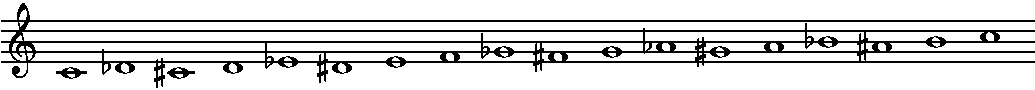
\includegraphics[width=\textwidth]{baglama_fifths_notation.pdf}
\caption{Keyboard mapping of Wilson's baglama scale with notation based on a
chain of keyboard fifths.}
\label{fig:baglama-fifths}
\end{figure}

Taking the comma step $(e, f) = (0, 1)$, we can use slashes to get an
alternative notation for the same keyboard mapping, shown in Figure
\ref{fig:baglama-slashes}. In this notation E\textbackslash{}\intervalsep{}E,
A\textbackslash{}\intervalsep{}A, and B\textbackslash{}\intervalsep{}B are all
intervals of 81/80, consistent with Bosanquet's notation. But also
D\textbackslash{}\intervalsep{}D and G\textbackslash{}\intervalsep{}G are
intervals of 33/32. The point is that a slash in this notation corresponds to a
particular move on the keyboard, here $(0, 1)$, not a particular interval. This
allows using only sharps/flats and slashes to notate a wide range of scales.
Looking at the notation on the stave, using the slashes here gives a smoothly
ascending scale.

\begin{figure}
\begin{center}
$\begin{NiceArray}[first-col, last-row, columns-width=1.4cm]{|c|c|c|c|c|c|}
\hline
 &
 &
 &    \scriptstyle \mathrm{G}\musFlat
 &    \scriptstyle \mathrm{A}\musFlat
 &    \scriptstyle \mathrm{B}\musFlat
 &    \scriptstyle \mathrm{C}
\\
2 &
 &
 &    1024/729
 &    128/81
 &    16/9
 &    2/1
\\
 &
 &
 &    \scriptstyle 588
 &    \scriptstyle 792
 &    \scriptstyle 996
 &    \scriptstyle 1200
\\
\hline
 &    \scriptstyle \mathrm{D}\musFlat
 &    \scriptstyle \mathrm{E}\musFlat
 &    \scriptstyle \mathrm{F}
 &    \scriptstyle \mathrm{G}
 &    \scriptstyle \mathrm{A}
 &    \scriptstyle \mathrm{B}
\\
1 &    256/243
 &    32/27
 &    4/3
 &    3/2
 &    27/16
 &    243/128
\\
 &    \scriptstyle 90
 &    \scriptstyle 294
 &    \scriptstyle 498
 &    \scriptstyle 702
 &    \scriptstyle 906
 &    \scriptstyle 1110
\\
\hline
 &    \scriptstyle \mathrm{C}
 &    \scriptstyle \mathrm{D}
 &    \scriptstyle \mathrm{E}
 &    \scriptstyle \mathrm{G}\raisebox{.2\height}{\scalebox{.55}{\textbf{\textbackslash}}}
 &    \scriptstyle \mathrm{A}\raisebox{.2\height}{\scalebox{.55}{\textbf{\textbackslash}}}
 &    \scriptstyle \mathrm{B}\raisebox{.2\height}{\scalebox{.55}{\textbf{\textbackslash}}}
\\
0 &    1/1
 &    9/8
 &    81/64
 &    16/11
 &    5/3
 &    15/8
\\
 &    \scriptstyle 0
 &    \scriptstyle 204
 &    \scriptstyle 408
 &    \scriptstyle 649
 &    \scriptstyle 884
 &    \scriptstyle 1088
\\
\hline
 &
 &    \scriptstyle \mathrm{D}\raisebox{.2\height}{\scalebox{.55}{\textbf{\textbackslash}}}
 &    \scriptstyle \mathrm{E}\raisebox{.2\height}{\scalebox{.55}{\textbf{\textbackslash}}}
 &
 &
 &
\\
-1 &
 &    12/11
 &    5/4
 &
 &
 &
\\
 &
 &    \scriptstyle 151
 &    \scriptstyle 386
 &
 &
 &
\\
\hline
& 0 & 1 & 2 & 3 & 4 & 5
\end{NiceArray}$
\end{center}

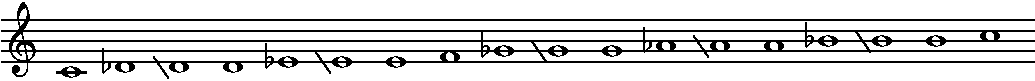
\includegraphics[width=\textwidth]{baglama_fifths_notation_2.pdf}
\caption{Keyboard mapping of Wilson's baglama scale notated using slashes.}
\label{fig:baglama-slashes}
\end{figure}

\clearpage
In the keyboard mapping of Figures \ref{fig:baglama-fifths} and
\ref{fig:baglama-slashes} we didn't need to use slashes; $\mathrm{C}\sharp$ and
$\mathrm{D\backslash}$ were enharmonically equivalent names for 12/11. But for
keyboard mappings in which 3/2 and 2/1 don't form a basis, some notes require
slashes to notate. Figure \ref{fig:baglama-thirds-and-fifths} shows such a
mapping for Wilson's baglama scale. In this mapping the fifth is at $(a, b) =
(1, 2)$, the octave is at $(c, d) = (1, 4)$, and the comma step is $(e, f) =
(1, -1)$. The keyboard is split into two chains of fifths, the even numbered
rows and the odd numbered rows, and the odd numbered rows require one
\textbackslash{} in their note names. In general if the fifth is at $(a, b)$
and the octave is at $(c, d)$, $ad - bc$ gives the number of chains of fifths
the keyboard will be split into \cite[14]{cassels1959geometry}, and indeed in
this case $ad - bc = 2$. This is useful since it tells us how many slashes will
be required in the notation.

\begin{figure}
\input{baglama_thirds_and_fifths.mathrm.tex}
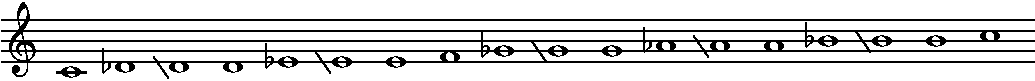
\includegraphics[width=\textwidth]{baglama2.preview.pdf}
\caption{Keyboard mapping of Wilson's baglama scale with a basis of 5/4 and 3/2.}
\label{fig:baglama-thirds-and-fifths}
\end{figure}

Figure \ref{fig:partch-notation} shows a notation for the keyboard mapping of
Partch's scale from Figure \ref{fig:harmonic-template-mapping}. Here the fifth
is at $(a, b) = (3, 3)$, the octave is $(c, d) = (6, 5)$, and the comma step is
$(e, f) = (1, 0)$. In this case $ad-bc = -3$, so the keyboard is split into
three chains of fifths, and we can notate it with three different numbers of
slashes (\textbackslash{}, none, and /). Compare Wilson's notation for Partch's
scale in \cite{wilson1975development}.

\clearpage
\begin{figure}
\begin{center}
$\begin{NiceArray}[first-col, last-row, columns-width=1.1cm]{|c|c|c|c|c|c|c|c|c|c|c|}
\hline
 &
 &
 &    \scriptstyle \mathrm{A}\musSharp
 &
 &    \scriptstyle \mathrm{B}\raisebox{.2\height}{\scalebox{.55}{\textbf{\textbackslash}}}
 &    \scriptstyle \mathrm{B}
 &    \scriptstyle \mathrm{B}\raisebox{.2\height}{\scalebox{.55}{\textbf{/}}}
 &    \scriptstyle \mathrm{C}\raisebox{.2\height}{\scalebox{.55}{\textbf{\textbackslash}}}
 &    \scriptstyle \mathrm{C}
 &
 &
\\
5 &
 &
 &    20/11
 &
 &    15/8
 &    40/21
 &    64/33
 &    160/81
 &    2/1
 &
 &
\\
 &
 &
 &    \scriptstyle 1035
 &
 &    \scriptstyle 1088
 &    \scriptstyle 1116
 &    \scriptstyle 1147
 &    \scriptstyle 1178
 &    \scriptstyle 1200
 &
 &
\\
\hline
 &
 &
 &
 &    \scriptstyle \mathrm{G}\musSharp\raisebox{.2\height}{\scalebox{.55}{\textbf{/}}}
 &    \scriptstyle \mathrm{A}\raisebox{.2\height}{\scalebox{.55}{\textbf{\textbackslash}}}
 &    \scriptstyle \mathrm{A}
 &    \scriptstyle \mathrm{A}\raisebox{.2\height}{\scalebox{.55}{\textbf{/}}}
 &    \scriptstyle \mathrm{B}\musFlat\raisebox{.2\height}{\scalebox{.55}{\textbf{\textbackslash}}}
 &    \scriptstyle \mathrm{B}\musFlat
 &    \scriptstyle \mathrm{B}\musFlat\raisebox{.2\height}{\scalebox{.55}{\textbf{/}}}
 &    \scriptstyle \mathrm{C}\musFlat\raisebox{.2\height}{\scalebox{.55}{\textbf{\textbackslash}}}
\\
4 &
 &
 &
 &    18/11
 &    5/3
 &    27/16
 &    12/7
 &    7/4
 &    16/9
 &    9/5
 &    11/6
\\
 &
 &
 &
 &    \scriptstyle 853
 &    \scriptstyle 884
 &    \scriptstyle 906
 &    \scriptstyle 933
 &    \scriptstyle 969
 &    \scriptstyle 996
 &    \scriptstyle 1018
 &    \scriptstyle 1049
\\
\hline
 &
 &
 &    \scriptstyle \mathrm{F}\musSharp
 &    \scriptstyle \mathrm{F}\musSharp\raisebox{.2\height}{\scalebox{.55}{\textbf{/}}}
 &    \scriptstyle \mathrm{G}\raisebox{.2\height}{\scalebox{.55}{\textbf{\textbackslash}}}
 &    \scriptstyle \mathrm{G}
 &    \scriptstyle \mathrm{G}\raisebox{.2\height}{\scalebox{.55}{\textbf{/}}}
 &    \scriptstyle \mathrm{A}\musFlat\raisebox{.2\height}{\scalebox{.55}{\textbf{\textbackslash}}}
 &    \scriptstyle \mathrm{A}\musFlat
 &    \scriptstyle \mathrm{A}\musFlat\raisebox{.2\height}{\scalebox{.55}{\textbf{/}}}
 &
\\
3 &
 &
 &    10/7
 &    16/11
 &    40/27
 &    3/2
 &    32/21
 &    14/9
 &    11/7
 &    8/5
 &
\\
 &
 &
 &    \scriptstyle 618
 &    \scriptstyle 649
 &    \scriptstyle 680
 &    \scriptstyle 702
 &    \scriptstyle 729
 &    \scriptstyle 765
 &    \scriptstyle 782
 &    \scriptstyle 814
 &
\\
\hline
 &
 &    \scriptstyle \mathrm{E}\raisebox{.2\height}{\scalebox{.55}{\textbf{\textbackslash}}}
 &    \scriptstyle \mathrm{E}
 &    \scriptstyle \mathrm{E}\raisebox{.2\height}{\scalebox{.55}{\textbf{/}}}
 &    \scriptstyle \mathrm{F}\raisebox{.2\height}{\scalebox{.55}{\textbf{\textbackslash}}}
 &    \scriptstyle \mathrm{F}
 &    \scriptstyle \mathrm{F}\raisebox{.2\height}{\scalebox{.55}{\textbf{/}}}
 &    \scriptstyle \mathrm{G}\musFlat\raisebox{.2\height}{\scalebox{.55}{\textbf{\textbackslash}}}
 &    \scriptstyle \mathrm{G}\musFlat
 &
 &
\\
2 &
 &    5/4
 &    14/11
 &    9/7
 &    21/16
 &    4/3
 &    27/20
 &    11/8
 &    7/5
 &
 &
\\
 &
 &    \scriptstyle 386
 &    \scriptstyle 418
 &    \scriptstyle 435
 &    \scriptstyle 471
 &    \scriptstyle 498
 &    \scriptstyle 520
 &    \scriptstyle 551
 &    \scriptstyle 582
 &
 &
\\
\hline
 &    \scriptstyle \mathrm{C}\musSharp\raisebox{.2\height}{\scalebox{.55}{\textbf{/}}}
 &    \scriptstyle \mathrm{D}\raisebox{.2\height}{\scalebox{.55}{\textbf{\textbackslash}}}
 &    \scriptstyle \mathrm{D}
 &    \scriptstyle \mathrm{D}\raisebox{.2\height}{\scalebox{.55}{\textbf{/}}}
 &    \scriptstyle \mathrm{E}\musFlat\raisebox{.2\height}{\scalebox{.55}{\textbf{\textbackslash}}}
 &    \scriptstyle \mathrm{E}\musFlat
 &    \scriptstyle \mathrm{E}\musFlat\raisebox{.2\height}{\scalebox{.55}{\textbf{/}}}
 &    \scriptstyle \mathrm{F}\musFlat\raisebox{.2\height}{\scalebox{.55}{\textbf{\textbackslash}}}
 &
 &
 &
\\
1 &    12/11
 &    10/9
 &    9/8
 &    8/7
 &    7/6
 &    32/27
 &    6/5
 &    11/9
 &
 &
 &
\\
 &    \scriptstyle 151
 &    \scriptstyle 182
 &    \scriptstyle 204
 &    \scriptstyle 231
 &    \scriptstyle 267
 &    \scriptstyle 294
 &    \scriptstyle 316
 &    \scriptstyle 347
 &
 &
 &
\\
\hline
 &
 &
 &    \scriptstyle \mathrm{C}
 &    \scriptstyle \mathrm{C}\raisebox{.2\height}{\scalebox{.55}{\textbf{/}}}
 &    \scriptstyle \mathrm{D}\musFlat\raisebox{.2\height}{\scalebox{.55}{\textbf{\textbackslash}}}
 &    \scriptstyle \mathrm{D}\musFlat
 &    \scriptstyle \mathrm{D}\musFlat\raisebox{.2\height}{\scalebox{.55}{\textbf{/}}}
 &
 &    \scriptstyle \mathrm{E}\musDoubleFlat
 &
 &
\\
0 &
 &
 &    1/1
 &    81/80
 &    33/32
 &    21/20
 &    16/15
 &
 &    11/10
 &
 &
\\
 &
 &
 &    \scriptstyle 0
 &    \scriptstyle 22
 &    \scriptstyle 53
 &    \scriptstyle 84
 &    \scriptstyle 112
 &
 &    \scriptstyle 165
 &
 &
\\
\hline
& -2 & -1 & 0 & 1 & 2 & 3 & 4 & 5 & 6 & 7 & 8
\end{NiceArray}$
\end{center}

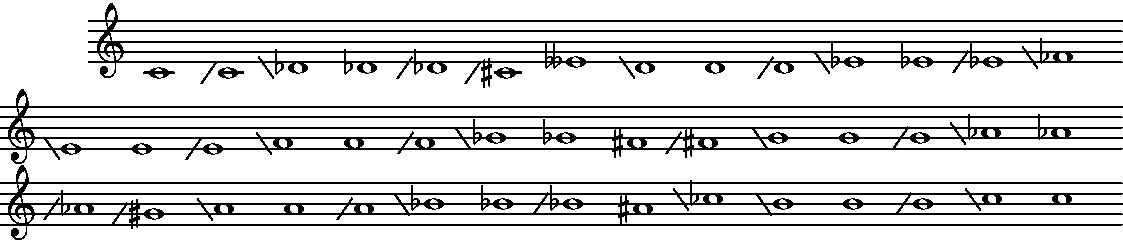
\includegraphics[width=\textwidth]{xen03-secor-partch-1.pdf}
\caption{Notation for a keyboard mapping of Partch's scale.\vspace{-0.05cm}}
\label{fig:partch-notation}
\end{figure}

Some keyboard mappings require a large number of slashes using this scheme. For
example Figure \ref{fig:hanson-no-tree} shows notation for a mapping of
Hanson's basic group of 19 tones. Here the fifth is at $(a, b) = (1, 2)$, the
octave is at $(c, d) = (-1, 4)$, and the comma step is $(e, f) = (5, -1)$. So
we have $ad - bc = 6$, and indeed we need six values of slashes (from $-3$,
\textbackslash{}\textbackslash{}\textbackslash{}, up to $+2$, //).

Wilson's tree notation \cite[40]{wilsonhebdomekontany} allows using less
slashes. Figure \ref{fig:hanson-tree} shows the mapping of Figure
\ref{fig:hanson-no-tree} with tree notation. The notation partners each
ordinary note ABCDEFG with a new `tree note' written abcdefg, with each
ordinary note and its tree note separated by a fixed step $(g, h)$ on the
keyboard (in Figure \ref{fig:hanson-tree} $(g, h) = (-4, 1)$). Then Equation
\ref{eq:notation} is extended to
\begin{align}
\begin{bmatrix}
    x \\
    y \\
\end{bmatrix}
    &=
u
\begin{bmatrix}
    a \\
    b \\
\end{bmatrix}
    +
v
\begin{bmatrix}
    c \\
    d \\
\end{bmatrix}
    +
w
\begin{bmatrix}
    e \\
    f \\
\end{bmatrix}
    +
t
\begin{bmatrix}
    g \\
    h \\
\end{bmatrix}
\label{eq:tree}
\end{align}
where $t$ can only be 0 or 1, and we use the ordinary note ABCDEFG if $t=0$ or
the tree note abcdefg if $t=1$. The idea is that with a good choice of tree
step $(g, h)$, we can use less slashes to reach some notes by first moving by
the tree step before moving by fifths, octaves, and commas. The tree note is
written in the same position on the stave as its ordinary partner but with a
different note head (triangular in Figure \ref{fig:hanson-tree}). Wilson also
gives the tree notes the long names ailm, beth, coll, duir, eadha, fearn, gort
from the Ogham alphabet (sometimes called the Celtic tree alphabet).

\begin{figure}
\begin{subfigure}{\textwidth}
\begin{center}
$\begin{NiceArray}[first-col, last-row, columns-width=1.4cm]{|c|c|c|c|c|c|}
\hline
 &    \scriptstyle \mathrm{C}\musFlat\raisebox{.2\height}{\scalebox{.55}{\textbf{/}}}\raisebox{.2\height}{\scalebox{.55}{\textbf{/}}}
 &    \scriptstyle \mathrm{C}
 &
 &
 &
 &
\\
4 &    48/25
 &    2/1
 &
 &
 &
 &
\\
 &    \scriptstyle 1129
 &    \scriptstyle 1200
 &
 &
 &
 &
\\
\hline
 &    \scriptstyle \mathrm{A}\musFlat\raisebox{.2\height}{\scalebox{.55}{\textbf{/}}}
 &    \scriptstyle \mathrm{A}\raisebox{.2\height}{\scalebox{.55}{\textbf{\textbackslash}}}
 &    \scriptstyle \mathrm{A}\musSharp\raisebox{.2\height}{\scalebox{.55}{\textbf{\textbackslash}}}\raisebox{.2\height}{\scalebox{.55}{\textbf{\textbackslash}}}\raisebox{.2\height}{\scalebox{.55}{\textbf{\textbackslash}}}
 &    \scriptstyle \mathrm{B}\musFlat\raisebox{.2\height}{\scalebox{.55}{\textbf{/}}}
 &    \scriptstyle \mathrm{B}\raisebox{.2\height}{\scalebox{.55}{\textbf{\textbackslash}}}
 &
\\
3 &    8/5
 &    5/3
 &    125/72
 &    9/5
 &    15/8
 &
\\
 &    \scriptstyle 814
 &    \scriptstyle 884
 &    \scriptstyle 955
 &    \scriptstyle 1018
 &    \scriptstyle 1088
 &
\\
\hline
 &    \scriptstyle \mathrm{F}
 &    \scriptstyle \mathrm{F}\musSharp\raisebox{.2\height}{\scalebox{.55}{\textbf{\textbackslash}}}\raisebox{.2\height}{\scalebox{.55}{\textbf{\textbackslash}}}
 &    \scriptstyle \mathrm{G}\musFlat\raisebox{.2\height}{\scalebox{.55}{\textbf{/}}}\raisebox{.2\height}{\scalebox{.55}{\textbf{/}}}
 &    \scriptstyle \mathrm{G}
 &    \scriptstyle \mathrm{G}\musSharp\raisebox{.2\height}{\scalebox{.55}{\textbf{\textbackslash}}}\raisebox{.2\height}{\scalebox{.55}{\textbf{\textbackslash}}}
 &
\\
2 &    4/3
 &    25/18
 &    36/25
 &    3/2
 &    25/16
 &
\\
 &    \scriptstyle 498
 &    \scriptstyle 569
 &    \scriptstyle 631
 &    \scriptstyle 702
 &    \scriptstyle 773
 &
\\
\hline
 &
 &    \scriptstyle \mathrm{D}\musSharp\raisebox{.2\height}{\scalebox{.55}{\textbf{\textbackslash}}}\raisebox{.2\height}{\scalebox{.55}{\textbf{\textbackslash}}}\raisebox{.2\height}{\scalebox{.55}{\textbf{\textbackslash}}}
 &    \scriptstyle \mathrm{E}\musFlat\raisebox{.2\height}{\scalebox{.55}{\textbf{/}}}
 &    \scriptstyle \mathrm{E}\raisebox{.2\height}{\scalebox{.55}{\textbf{\textbackslash}}}
 &    \scriptstyle \mathrm{E}\musSharp\raisebox{.2\height}{\scalebox{.55}{\textbf{\textbackslash}}}\raisebox{.2\height}{\scalebox{.55}{\textbf{\textbackslash}}}\raisebox{.2\height}{\scalebox{.55}{\textbf{\textbackslash}}}
 &
\\
1 &
 &    144/125
 &    6/5
 &    5/4
 &    125/96
 &
\\
 &
 &    \scriptstyle 245
 &    \scriptstyle 316
 &    \scriptstyle 386
 &    \scriptstyle 457
 &
\\
\hline
 &
 &
 &    \scriptstyle \mathrm{C}
 &    \scriptstyle \mathrm{C}\musSharp\raisebox{.2\height}{\scalebox{.55}{\textbf{\textbackslash}}}\raisebox{.2\height}{\scalebox{.55}{\textbf{\textbackslash}}}
 &    \scriptstyle \mathrm{D}\musFlat\raisebox{.2\height}{\scalebox{.55}{\textbf{/}}}\raisebox{.2\height}{\scalebox{.55}{\textbf{/}}}
 &    \scriptstyle \mathrm{D}
\\
0 &
 &
 &    1/1
 &    25/24
 &    27/25
 &    9/8
\\
 &
 &
 &    \scriptstyle 0
 &    \scriptstyle 71
 &    \scriptstyle 133
 &    \scriptstyle 204
\\
\hline
& -2 & -1 & 0 & 1 & 2 & 3
\end{NiceArray}$
\end{center}

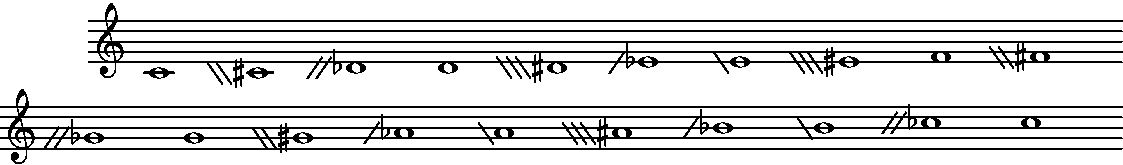
\includegraphics[width=\textwidth]{hanson-no-tree-notation.pdf}
\caption{Only sharps/flats and slashes}
\vspace{0.8cm}
\label{fig:hanson-no-tree}
\end{subfigure}
\begin{subfigure}{\textwidth}
\begin{center}
$\begin{NiceArray}[first-col, last-row, columns-width=1.4cm]{|c|c|c|c|c|c|}
\hline
 &    \scriptstyle \mathrm{b}\raisebox{.2\height}{\scalebox{.55}{\textbf{\textbackslash}}}
 &    \scriptstyle \mathrm{C}
 &
 &
 &
 &
\\
4 &    48/25
 &    2/1
 &
 &
 &
 &
\\
 &    \scriptstyle 1129
 &    \scriptstyle 1200
 &
 &
 &
 &
\\
\hline
 &    \scriptstyle \mathrm{A}\musFlat\raisebox{.2\height}{\scalebox{.55}{\textbf{/}}}
 &    \scriptstyle \mathrm{A}\raisebox{.2\height}{\scalebox{.55}{\textbf{\textbackslash}}}
 &    \scriptstyle \mathrm{a}
 &    \scriptstyle \mathrm{B}\musFlat\raisebox{.2\height}{\scalebox{.55}{\textbf{/}}}
 &    \scriptstyle \mathrm{B}\raisebox{.2\height}{\scalebox{.55}{\textbf{\textbackslash}}}
 &
\\
3 &    8/5
 &    5/3
 &    125/72
 &    9/5
 &    15/8
 &
\\
 &    \scriptstyle 814
 &    \scriptstyle 884
 &    \scriptstyle 955
 &    \scriptstyle 1018
 &    \scriptstyle 1088
 &
\\
\hline
 &    \scriptstyle \mathrm{F}
 &    \scriptstyle \mathrm{f}\raisebox{.2\height}{\scalebox{.55}{\textbf{/}}}
 &    \scriptstyle \mathrm{f}\musSharp\raisebox{.2\height}{\scalebox{.55}{\textbf{\textbackslash}}}
 &    \scriptstyle \mathrm{G}
 &    \scriptstyle \mathrm{g}\raisebox{.2\height}{\scalebox{.55}{\textbf{/}}}
 &
\\
2 &    4/3
 &    25/18
 &    36/25
 &    3/2
 &    25/16
 &
\\
 &    \scriptstyle 498
 &    \scriptstyle 569
 &    \scriptstyle 631
 &    \scriptstyle 702
 &    \scriptstyle 773
 &
\\
\hline
 &
 &    \scriptstyle \mathrm{d}
 &    \scriptstyle \mathrm{E}\musFlat\raisebox{.2\height}{\scalebox{.55}{\textbf{/}}}
 &    \scriptstyle \mathrm{E}\raisebox{.2\height}{\scalebox{.55}{\textbf{\textbackslash}}}
 &    \scriptstyle \mathrm{e}
 &
\\
1 &
 &    144/125
 &    6/5
 &    5/4
 &    125/96
 &
\\
 &
 &    \scriptstyle 245
 &    \scriptstyle 316
 &    \scriptstyle 386
 &    \scriptstyle 457
 &
\\
\hline
 &
 &
 &    \scriptstyle \mathrm{C}
 &    \scriptstyle \mathrm{c}\raisebox{.2\height}{\scalebox{.55}{\textbf{/}}}
 &    \scriptstyle \mathrm{c}\musSharp\raisebox{.2\height}{\scalebox{.55}{\textbf{\textbackslash}}}
 &    \scriptstyle \mathrm{D}
\\
0 &
 &
 &    1/1
 &    25/24
 &    27/25
 &    9/8
\\
 &
 &
 &    \scriptstyle 0
 &    \scriptstyle 71
 &    \scriptstyle 133
 &    \scriptstyle 204
\\
\hline
& -2 & -1 & 0 & 1 & 2 & 3
\end{NiceArray}$
\end{center}

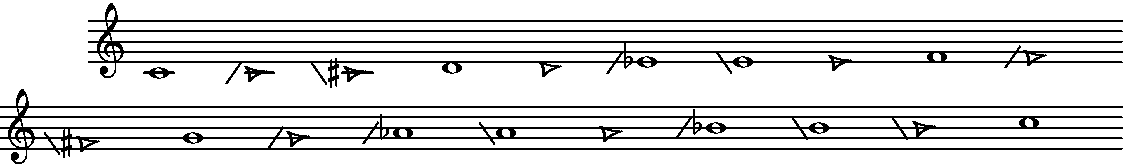
\includegraphics[width=\textwidth]{hanson-tree-notation.pdf}
\caption{Tree notation.}
\label{fig:hanson-tree}
\end{subfigure}
\caption{Notations for a mapping of Hanson's basic group of 19 tones.}
\end{figure}

I use Wilson's tree notation for my guitar tuned in Hanson temperament
\cite{hanson1989development}.\footnotemark{} This guitar has frets spaced third
tones of $9/8^{1/3}$ or 68 cents apart and strings tuned minor thirds of
$3^{1/6}$ or 317 cents apart. Since the notations of this section depend purely
on keyboard (or fretboard!) position, they can be applied to temperaments as
well as just scales. Figure \ref{fig:guitar-tree} shows the guitar fretboard
labeled with cent values and tree notation note names. Here a comma after a
cent value (e.g. $996,$) denotes lowering by an octave, an apostrophe (e.g.
$68'$) raising by an octave.
\footnotetext{You can hear the guitar in action in the 8th International
Microtonal Guitar Competition here
\url{https://www.youtube.com/watch?v=cc8hbiXu3b0}}

\begin{figure}
\begin{center}
$\begin{NiceArray}[first-col, last-row, columns-width=1.1cm]{|c|c|c|c|c|c|c|c|c|c|c|}
\hline
 &\cellcolor{gray!25}     \scriptstyle 
 &\cellcolor{gray!25}     \scriptstyle 
 &    \scriptstyle 
 &\cellcolor{gray!25}     \scriptstyle 
 &\cellcolor{gray!25}     \scriptstyle 
 &    \scriptstyle 
 &\cellcolor{gray!25}     \scriptstyle 
 &\cellcolor{gray!25}     \scriptstyle 
 &    \scriptstyle 
 &\cellcolor{gray!25}     \scriptstyle 
 &\cellcolor{gray!25}     \scriptstyle 
\\
4 &\cellcolor{gray!25}     \mathrm{b}\musFlat\raisebox{.2\height}{\scalebox{.7}{\textbf{/}}}
 &\cellcolor{gray!25}     \mathrm{b}\raisebox{.2\height}{\scalebox{.7}{\textbf{\textbackslash}}}
 &    \mathrm{C}
 &\cellcolor{gray!25}     \mathrm{c}\raisebox{.2\height}{\scalebox{.7}{\textbf{/}}}
 &\cellcolor{gray!25}     \mathrm{c}\musSharp\raisebox{.2\height}{\scalebox{.7}{\textbf{\textbackslash}}}
 &    \mathrm{D}
 &\cellcolor{gray!25}     \mathrm{d}\raisebox{.2\height}{\scalebox{.7}{\textbf{/}}}
 &\cellcolor{gray!25}     \mathrm{d}\musSharp\raisebox{.2\height}{\scalebox{.7}{\textbf{\textbackslash}}}
 &    \mathrm{E}
 &\cellcolor{gray!25}     \mathrm{e}\raisebox{.2\height}{\scalebox{.7}{\textbf{/}}}
 &\cellcolor{gray!25}     \mathrm{e}\musSharp\raisebox{.2\height}{\scalebox{.7}{\textbf{\textbackslash}}}
\\
 &\cellcolor{gray!25}     \scriptstyle 1064
 &\cellcolor{gray!25}     \scriptstyle 1132
 &    \scriptstyle 0'
 &\cellcolor{gray!25}     \scriptstyle 68'
 &\cellcolor{gray!25}     \scriptstyle 136'
 &    \scriptstyle 204'
 &\cellcolor{gray!25}     \scriptstyle 272'
 &\cellcolor{gray!25}     \scriptstyle 340'
 &    \scriptstyle 408'
 &\cellcolor{gray!25}     \scriptstyle 476'
 &\cellcolor{gray!25}     \scriptstyle 544'
\\
\hline
 &\cellcolor{gray!25}     \scriptstyle 
 &    \scriptstyle 
 &    \scriptstyle 
 &\cellcolor{gray!25}     \scriptstyle 
 &    \scriptstyle 
 &    \scriptstyle 
 &\cellcolor{gray!25}     \scriptstyle 
 &    \scriptstyle 
 &    \scriptstyle 
 &\cellcolor{gray!25}     \scriptstyle 
 &    \scriptstyle 
\\
3 &\cellcolor{gray!25}     \mathrm{g}
 &    \mathrm{A}\musFlat\raisebox{.2\height}{\scalebox{.7}{\textbf{/}}}
 &    \mathrm{A}\raisebox{.2\height}{\scalebox{.7}{\textbf{\textbackslash}}}
 &\cellcolor{gray!25}     \mathrm{a}
 &    \mathrm{B}\musFlat\raisebox{.2\height}{\scalebox{.7}{\textbf{/}}}
 &    \mathrm{B}\raisebox{.2\height}{\scalebox{.7}{\textbf{\textbackslash}}}
 &\cellcolor{gray!25}     \mathrm{b}
 &    \mathrm{C}\raisebox{.2\height}{\scalebox{.7}{\textbf{/}}}
 &    \mathrm{C}\musSharp\raisebox{.2\height}{\scalebox{.7}{\textbf{\textbackslash}}}
 &\cellcolor{gray!25}     \mathrm{c}\musSharp
 &    \mathrm{D}\raisebox{.2\height}{\scalebox{.7}{\textbf{/}}}
\\
 &\cellcolor{gray!25}     \scriptstyle 747
 &    \scriptstyle 815
 &    \scriptstyle 883
 &\cellcolor{gray!25}     \scriptstyle 951
 &    \scriptstyle 1019
 &    \scriptstyle 1087
 &\cellcolor{gray!25}     \scriptstyle 1155
 &    \scriptstyle 23'
 &    \scriptstyle 91'
 &\cellcolor{gray!25}     \scriptstyle 159'
 &    \scriptstyle 227'
\\
\hline
 &\cellcolor{gray!25}     \scriptstyle 
 &    \scriptstyle 
 &\cellcolor{gray!25}     \scriptstyle 
 &\cellcolor{gray!25}     \scriptstyle 
 &    \scriptstyle 
 &\cellcolor{gray!25}     \scriptstyle 
 &\cellcolor{gray!25}     \scriptstyle 
 &    \scriptstyle 
 &\cellcolor{gray!25}     \scriptstyle 
 &\cellcolor{gray!25}     \scriptstyle 
 &    \scriptstyle 
\\
2 &\cellcolor{gray!25}     \mathrm{e}\raisebox{.2\height}{\scalebox{.7}{\textbf{\textbackslash}}}
 &    \mathrm{F}
 &\cellcolor{gray!25}     \mathrm{f}\raisebox{.2\height}{\scalebox{.7}{\textbf{/}}}
 &\cellcolor{gray!25}     \mathrm{f}\musSharp\raisebox{.2\height}{\scalebox{.7}{\textbf{\textbackslash}}}
 &    \mathrm{G}
 &\cellcolor{gray!25}     \mathrm{g}\raisebox{.2\height}{\scalebox{.7}{\textbf{/}}}
 &\cellcolor{gray!25}     \mathrm{g}\musSharp\raisebox{.2\height}{\scalebox{.7}{\textbf{\textbackslash}}}
 &    \mathrm{A}
 &\cellcolor{gray!25}     \mathrm{a}\raisebox{.2\height}{\scalebox{.7}{\textbf{/}}}
 &\cellcolor{gray!25}     \mathrm{a}\musSharp\raisebox{.2\height}{\scalebox{.7}{\textbf{\textbackslash}}}
 &    \mathrm{B}
\\
 &\cellcolor{gray!25}     \scriptstyle 430
 &    \scriptstyle 498
 &\cellcolor{gray!25}     \scriptstyle 566
 &\cellcolor{gray!25}     \scriptstyle 634
 &    \scriptstyle 702
 &\cellcolor{gray!25}     \scriptstyle 770
 &\cellcolor{gray!25}     \scriptstyle 838
 &    \scriptstyle 906
 &\cellcolor{gray!25}     \scriptstyle 974
 &\cellcolor{gray!25}     \scriptstyle 1042
 &    \scriptstyle 1110
\\
\hline
 &    \scriptstyle 
 &    \scriptstyle 
 &\cellcolor{gray!25}     \scriptstyle 
 &    \scriptstyle 
 &    \scriptstyle 
 &\cellcolor{gray!25}     \scriptstyle 
 &    \scriptstyle 
 &    \scriptstyle 
 &\cellcolor{gray!25}     \scriptstyle 
 &    \scriptstyle 
 &    \scriptstyle 
\\
1 &    \mathrm{D}\musFlat\raisebox{.2\height}{\scalebox{.7}{\textbf{/}}}
 &    \mathrm{D}\raisebox{.2\height}{\scalebox{.7}{\textbf{\textbackslash}}}
 &\cellcolor{gray!25}     \mathrm{d}
 &    \mathrm{E}\musFlat\raisebox{.2\height}{\scalebox{.7}{\textbf{/}}}
 &    \mathrm{E}\raisebox{.2\height}{\scalebox{.7}{\textbf{\textbackslash}}}
 &\cellcolor{gray!25}     \mathrm{e}
 &    \mathrm{F}\raisebox{.2\height}{\scalebox{.7}{\textbf{/}}}
 &    \mathrm{F}\musSharp\raisebox{.2\height}{\scalebox{.7}{\textbf{\textbackslash}}}
 &\cellcolor{gray!25}     \mathrm{f}\musSharp
 &    \mathrm{G}\raisebox{.2\height}{\scalebox{.7}{\textbf{/}}}
 &    \mathrm{G}\musSharp\raisebox{.2\height}{\scalebox{.7}{\textbf{\textbackslash}}}
\\
 &    \scriptstyle 113
 &    \scriptstyle 181
 &\cellcolor{gray!25}     \scriptstyle 249
 &    \scriptstyle 317
 &    \scriptstyle 385
 &\cellcolor{gray!25}     \scriptstyle 453
 &    \scriptstyle 521
 &    \scriptstyle 589
 &\cellcolor{gray!25}     \scriptstyle 657
 &    \scriptstyle 725
 &    \scriptstyle 793
\\
\hline
 &    \scriptstyle 
 &\cellcolor{gray!25}     \scriptstyle 
 &\cellcolor{gray!25}     \scriptstyle 
 &    \scriptstyle 
 &\cellcolor{gray!25}     \scriptstyle 
 &\cellcolor{gray!25}     \scriptstyle 
 &    \scriptstyle 
 &\cellcolor{gray!25}     \scriptstyle 
 &\cellcolor{gray!25}     \scriptstyle 
 &    \scriptstyle 
 &\cellcolor{gray!25}     \scriptstyle 
\\
0 &    \mathrm{B}\musFlat
 &\cellcolor{gray!25}     \mathrm{b}\musFlat\raisebox{.2\height}{\scalebox{.7}{\textbf{/}}}
 &\cellcolor{gray!25}     \mathrm{b}\raisebox{.2\height}{\scalebox{.7}{\textbf{\textbackslash}}}
 &    \mathrm{C}
 &\cellcolor{gray!25}     \mathrm{c}\raisebox{.2\height}{\scalebox{.7}{\textbf{/}}}
 &\cellcolor{gray!25}     \mathrm{c}\musSharp\raisebox{.2\height}{\scalebox{.7}{\textbf{\textbackslash}}}
 &    \mathrm{D}
 &\cellcolor{gray!25}     \mathrm{d}\raisebox{.2\height}{\scalebox{.7}{\textbf{/}}}
 &\cellcolor{gray!25}     \mathrm{d}\musSharp\raisebox{.2\height}{\scalebox{.7}{\textbf{\textbackslash}}}
 &    \mathrm{E}
 &\cellcolor{gray!25}     \mathrm{e}\raisebox{.2\height}{\scalebox{.7}{\textbf{/}}}
\\
 &    \scriptstyle 996,
 &\cellcolor{gray!25}     \scriptstyle 1064,
 &\cellcolor{gray!25}     \scriptstyle 1132,
 &    \scriptstyle 0
 &\cellcolor{gray!25}     \scriptstyle 68
 &\cellcolor{gray!25}     \scriptstyle 136
 &    \scriptstyle 204
 &\cellcolor{gray!25}     \scriptstyle 272
 &\cellcolor{gray!25}     \scriptstyle 340
 &    \scriptstyle 408
 &\cellcolor{gray!25}     \scriptstyle 476
\\
\hline
 &    \scriptstyle 
 &\cellcolor{gray!25}     \scriptstyle 
 &    \scriptstyle 
 &    \scriptstyle 
 &\cellcolor{gray!25}     \scriptstyle 
 &    \scriptstyle 
 &    \scriptstyle 
 &\cellcolor{gray!25}     \scriptstyle 
 &    \scriptstyle 
 &    \scriptstyle 
 &\cellcolor{gray!25}     \scriptstyle 
\\
-1 &    \mathrm{G}\raisebox{.2\height}{\scalebox{.7}{\textbf{\textbackslash}}}
 &\cellcolor{gray!25}     \mathrm{g}
 &    \mathrm{A}\musFlat\raisebox{.2\height}{\scalebox{.7}{\textbf{/}}}
 &    \mathrm{A}\raisebox{.2\height}{\scalebox{.7}{\textbf{\textbackslash}}}
 &\cellcolor{gray!25}     \mathrm{a}
 &    \mathrm{B}\musFlat\raisebox{.2\height}{\scalebox{.7}{\textbf{/}}}
 &    \mathrm{B}\raisebox{.2\height}{\scalebox{.7}{\textbf{\textbackslash}}}
 &\cellcolor{gray!25}     \mathrm{b}
 &    \mathrm{C}\raisebox{.2\height}{\scalebox{.7}{\textbf{/}}}
 &    \mathrm{C}\musSharp\raisebox{.2\height}{\scalebox{.7}{\textbf{\textbackslash}}}
 &\cellcolor{gray!25}     \mathrm{c}\musSharp
\\
 &    \scriptstyle 679,
 &\cellcolor{gray!25}     \scriptstyle 747,
 &    \scriptstyle 815,
 &    \scriptstyle 883,
 &\cellcolor{gray!25}     \scriptstyle 951,
 &    \scriptstyle 1019,
 &    \scriptstyle 1087,
 &\cellcolor{gray!25}     \scriptstyle 1155,
 &    \scriptstyle 23
 &    \scriptstyle 91
 &\cellcolor{gray!25}     \scriptstyle 159
\\
\hline
& -3 & -2 & -1 & 0 & 1 & 2 & 3 & 4 & 5 & 6 & 7
\end{NiceArray}$
\end{center}

\caption{Hanson guitar fretboard with tree notation.}
\label{fig:guitar-tree}
\end{figure}

\begin{figure}
\centering
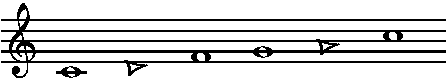
\includegraphics[]{pentatonic.cropped.pdf}
\caption{A pentatonic scale built by splitting the perfect fourth written in tree notation.}
\label{fig:pentatonic}
\end{figure}

It's convenient being able to write any note on the fretboard with at most one
slash. I also like that the pentatonic scale built from split perfect fourths,
Figure \ref{fig:pentatonic}, has a simple notation; this scale feels and sounds
very natural to me on this Hanson guitar.

I do find the tree notes themselves quite musically suggestive. As it happens
the intervals from C written with ordinary notes sound more familiar to me,
while the tree notes are less familiar, as you can perhaps imagine from the
cents values in Figure \ref{fig:guitar-tree}. You could take this too far but
on this fretboard I sometimes think of the tree notes as another world to
explore, and the notation feels like an invitation to do this.

\clearpage
If we choose the tree step $(g, h)$ to connect $\mathrm{B}$ to
$\mathrm{B}\flat$, Wilson's tree notation reproduces his notations from
\textit{On linear notations and the Bosanquet keyboard}
\cite{wilson1975linear}. This is surprising since their motivations are
apparently quite different. In \textit{Linear notations} Wilson uses an
extended set of note names (or nominals) when naming the chain of fifths, shown
in Table \ref{tab:wilson}. The chain positions $-6$ to $+6$ are named $\gamma$,
$\delta$, $\alpha$, $\epsilon$, $\beta$, F, C, G, D, A, E, B, and H. In
principle you could extend Table \ref{tab:wilson} by adding sharps and flats as
in Table \ref{tab:fifths}, but in \textit{Linear notations} Wilson uses (in the
terminology of this section) the slash exclusively, giving notations using only
one pair of accidentals.

\begin{table}
\begin{center}
\begin{tabular}{l|rrrrrrrrrrrrrrrrrr}
\toprule
Fifths & $-6$ & $-5$ & $-4$ & $-3$ & $-2$ & $-1$ & $\ \:0$ & $+1$ & $+2$ & $+3$ & $+4$ & $+5$ & $+6$ \\
Name & $\gamma$ & $\delta$ & $\alpha$ & $\epsilon$ & $\beta$ & F & C & G & D & A & E & B & H \\
\bottomrule
\end{tabular}
\end{center}
\caption{Wilson's extended nominals.}
\label{tab:wilson}
\end{table}

Figure \ref{fig:negative-notation} shows Wilson's mapping of a 31-tone scale
notated with twelve note names \cite[8]{wilson1975development}. The steps
between B and $\beta$, E and $\epsilon$, A and $\alpha$, D and $\delta$, and G
and $\gamma$ are all $(-1, 1)$, so the notation is in fact identical with tree
notation with the tree step $(-1, 1)$. Here the tree notes b e a d g correspond
to the extended nominals $\beta$ $\epsilon$ $\alpha$ $\delta$ $\gamma$ and the
ordinary notes $\mathrm{B}\flat$ $\mathrm{E}\flat$ $\mathrm{A}\flat$
$\mathrm{D}\flat$ $\mathrm{G}\flat$. In fact this is true for all
\textit{Linear notations} style notations, so long as they use 14 or less
nominals (Wilson discusses at most 13). One difference is the use of H for
chain position $+6$; in tree notation we instead get a c at chain position
$-7$, which would correspond to say a $\kappa$ at chain position $-7$ in Table
\ref{tab:wilson}. Figure \ref{fig:negative-notation} shows the extended-nominal
notes with a different note head on the stave; in \textit{Linear notations}
Wilson discusses this but primarily uses extended staves which show ordinary
notes on spaces and extended-nominal notes on lines.

\begin{figure}
\begin{center}
$\begin{NiceArray}[first-col, last-row, columns-width=1.4cm]{|c|c|c|c|c|c|c|c|}
\hline
 &
 &
 &    \scriptstyle \gamma\raisebox{.2\height}{\scalebox{.55}{\textbf{/}}}
 &    \scriptstyle \alpha\raisebox{.2\height}{\scalebox{.55}{\textbf{/}}}
 &    \scriptstyle \beta\raisebox{.2\height}{\scalebox{.55}{\textbf{/}}}
 &
 &
 &
\\
4 &
 &
 &    16/11
 &    18/11
 &    81/44
 &
 &
 &
\\
 &
 &
 &    \scriptstyle 649
 &    \scriptstyle 853
 &    \scriptstyle 1056
 &
 &
 &
\\
\hline
 &    \scriptstyle \delta\raisebox{.2\height}{\scalebox{.55}{\textbf{/}}}
 &    \scriptstyle \epsilon\raisebox{.2\height}{\scalebox{.55}{\textbf{/}}}
 &    \scriptstyle \mathrm{F}\raisebox{.2\height}{\scalebox{.55}{\textbf{/}}}
 &    \scriptstyle \mathrm{G}\raisebox{.2\height}{\scalebox{.55}{\textbf{/}}}
 &    \scriptstyle \mathrm{A}\raisebox{.2\height}{\scalebox{.55}{\textbf{/}}}
 &    \scriptstyle \mathrm{B}\raisebox{.2\height}{\scalebox{.55}{\textbf{/}}}
 &
 &
\\
3 &    12/11
 &    27/22
 &    256/189
 &    32/21
 &    12/7
 &    40/21
 &
 &
\\
 &    \scriptstyle 151
 &    \scriptstyle 354
 &    \scriptstyle 525
 &    \scriptstyle 729
 &    \scriptstyle 933
 &    \scriptstyle 1116
 &
 &
\\
\hline
 &    \scriptstyle \mathrm{C}\raisebox{.2\height}{\scalebox{.55}{\textbf{/}}}
 &    \scriptstyle \mathrm{D}\raisebox{.2\height}{\scalebox{.55}{\textbf{/}}}
 &    \scriptstyle \mathrm{E}\raisebox{.2\height}{\scalebox{.55}{\textbf{/}}}
 &    \scriptstyle \gamma
 &    \scriptstyle \alpha
 &    \scriptstyle \beta
 &    \scriptstyle \mathrm{C}
 &
\\
2 &    64/63
 &    8/7
 &    80/63
 &    64/45
 &    8/5
 &    9/5
 &    2/1
 &
\\
 &    \scriptstyle 27
 &    \scriptstyle 231
 &    \scriptstyle 414
 &    \scriptstyle 610
 &    \scriptstyle 814
 &    \scriptstyle 1018
 &    \scriptstyle 1200
 &
\\
\hline
 &
 &    \scriptstyle \delta
 &    \scriptstyle \epsilon
 &    \scriptstyle \mathrm{F}
 &    \scriptstyle \mathrm{G}
 &    \scriptstyle \mathrm{A}
 &    \scriptstyle \mathrm{B}
 &
\\
1 &
 &    16/15
 &    6/5
 &    4/3
 &    3/2
 &    27/16
 &    15/8
 &
\\
 &
 &    \scriptstyle 112
 &    \scriptstyle 316
 &    \scriptstyle 498
 &    \scriptstyle 702
 &    \scriptstyle 906
 &    \scriptstyle 1088
 &
\\
\hline
 &
 &    \scriptstyle \mathrm{C}
 &    \scriptstyle \mathrm{D}
 &    \scriptstyle \mathrm{E}
 &    \scriptstyle \gamma\raisebox{.2\height}{\scalebox{.55}{\textbf{\textbackslash}}}
 &    \scriptstyle \alpha\raisebox{.2\height}{\scalebox{.55}{\textbf{\textbackslash}}}
 &    \scriptstyle \beta\raisebox{.2\height}{\scalebox{.55}{\textbf{\textbackslash}}}
 &    \scriptstyle \mathrm{C}\raisebox{.2\height}{\scalebox{.55}{\textbf{\textbackslash}}}
\\
0 &
 &    1/1
 &    9/8
 &    5/4
 &    112/81
 &    14/9
 &    7/4
 &    35/18
\\
 &
 &    \scriptstyle 0
 &    \scriptstyle 204
 &    \scriptstyle 386
 &    \scriptstyle 561
 &    \scriptstyle 765
 &    \scriptstyle 969
 &    \scriptstyle 1151
\\
\hline
 &
 &
 &    \scriptstyle \delta\raisebox{.2\height}{\scalebox{.55}{\textbf{\textbackslash}}}
 &    \scriptstyle \epsilon\raisebox{.2\height}{\scalebox{.55}{\textbf{\textbackslash}}}
 &    \scriptstyle \mathrm{F}\raisebox{.2\height}{\scalebox{.55}{\textbf{\textbackslash}}}
 &
 &
 &
\\
-1 &
 &
 &    28/27
 &    7/6
 &    35/27
 &
 &
 &
\\
 &
 &
 &    \scriptstyle 63
 &    \scriptstyle 267
 &    \scriptstyle 449
 &
 &
 &
\\
\hline
& -1 & 0 & 1 & 2 & 3 & 4 & 5 & 6
\end{NiceArray}$
\end{center}

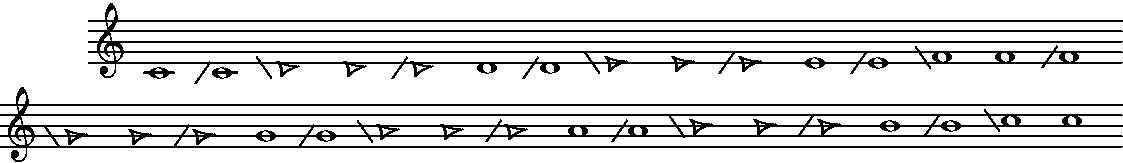
\includegraphics[width=\textwidth]{xen03-wilson-negative-31.wilson.cropped.pdf}
\caption{Notation for Wilson's Genus 31 using extended nominals.}
\label{fig:negative-notation}
\end{figure}

To connect this section's Equation \ref{eq:notation} with Wilson's
\textit{Linear notations} paper, note that all mappings in \textit{Linear
notations} use a $4/7$ keyboard, and so have a basis of $(a, b) = (1, 3)$, $(c,
d) = (2, 5)$, where the fifth and octave are placed. Table \ref{tab:comma}
gives the comma step $(e, f)$ for each notation in \textit{Linear notations}.
Table \ref{tab:comma} also shows the chain coordinates $(p, q)$ of each comma
step, and the name for the notation given by Wilson. The name is determined by
the number of fifths $p$, e.g. $+7$ is septimally positive, $-5$ is quintally
negative, and so on. Wilson uses different accidentals for each system, to
indicate that the commas span different numbers of fifths.

Table \ref{tab:comma} also gives the example temperaments shown on each of
Wilson's notation diagrams in $\textit{Linear notations}$. The comma step
always goes up one degree of all the temperaments on each diagram. An example
of say 10/17 means 17 tone equal temperament, with the fifth at degree 10. You
can check that for an example $m/n$, we always have $p m \equiv 1 \pmod{n}$,
where $p$ is the number of fifths spanned by the comma, e.g. for the 10/17
example for Duodecimally positive notation we have $12 \cdot 10 \equiv 1
\pmod{17}$.

Wilson combines tree notation and extended nominals for his septendene
\cite{wilson1977septendene}, notating this 17-tone scale with no accidentals
(compare \cite{wilson1980design}). The note names are consistent with Equation
\ref{eq:tree} used together with Table \ref{tab:wilson}.

\begin{table}
\centering
\begin{tabular}{rr@{\hspace{1cm}}rr@{\hspace{1cm}}l@{\hspace{1cm}}rrrr}
\toprule
$e$ &   $f$ &   $p$ &   $q$ &   Name    &   \multicolumn{4}{l}{\hspace{-0.2cm}Examples} \\
\midrule
$-2$    &   $1$   &   $12$  &   $-7$  &   Duodecimally positive   &   10/17 &  17/29 &  24/41 & \\
$2$ &   $-1$   &   $-12$    &   $7$  &   Duodecimally negative   &   11/19 &  18/31 &  25/43 & \\
$-1$    &   $1$   &   $7$   &   $-4$   &   Septimally positive     &   7/12 &  11/19 &  15/26  & \\
$1$ &   $-1$   &   $-7$ &   $4$   &   Septimally negative     &   5/9 &  9/16 &  13/23    & \\
$-1$    &   $0$   &   $5$   &   $-3$   &   Quintally positive      &   5/8 &  8/13 &  11/18 &  14/23 \\
$1$ &   $0$    &   $-5$ &   $3$   &   Quintally negative      &   4/7 &  7/12 &  10/17 &  13/22 \\
\bottomrule
\end{tabular}
\caption{The comma steps used in Wilson's \textit{Linear notations}.}
\label{tab:comma}
\end{table}

\clearpage
\section{Playing the keyboard mappings}
\label{playing}
I play the keyboard mappings on a Novation Launchpad X, a relatively affordable
MIDI grid controller. This section describes some of the practicalities of
actually doing this.

There are at least three ways to get each key on the Launchpad to play the
desired note in the keyboard mapping. One way is to use the Novation Components
software, which allows specifying the MIDI note sent by each key. This has the
advantage that once you've set up a mapping, no software is required.  The
second way is to remap the MIDI notes sent by the Launchpad in software, for
example using a MIDI remapper plugin in a DAW (digital audio workstation). This
makes it quick to try out different mappings. The third way is to use
MTS\nobreakdash-ESP, a library for setting a shared tuning for different music
software, to directly specify the frequency for each Launchpad key. The point
here is that MTS-ESP provides a tuning table which maps each MIDI note to a
frequency, so you can set the tuning for a scale and map it to the Launchpad
`in one go' with a suitable tuning table. I find the MTS-ESP way particularly
convenient since it doesn't require receiving and resending MIDI messages. For
this purpose the \texttt{mtsespy} Python wrapper for MTS-ESP may be of
interest.\footnote{Available at \url{https://github.com/narenratan/mtsespy}}

The keys of the Launchpad can be lit up in various colors. This can be done in
the Novation Components software or by sending MIDI messages to the Launchpad
\cite{launchpad}. I find the key lighting genuinely useful for playing Wilson's
keyboard mappings. I tend to light up all mapped keys white, with the harmonic
template lit in blue. Figure \ref{fig:launchpad} shows the Launchpad set up to
play the keyboard mapping from Figure \ref{fig:dal-reduced}. I find that the
harmonic template together with the often irregular outline of the keyboard
mapping give enough visual cues to find the notes I'm after.

\begin{figure}
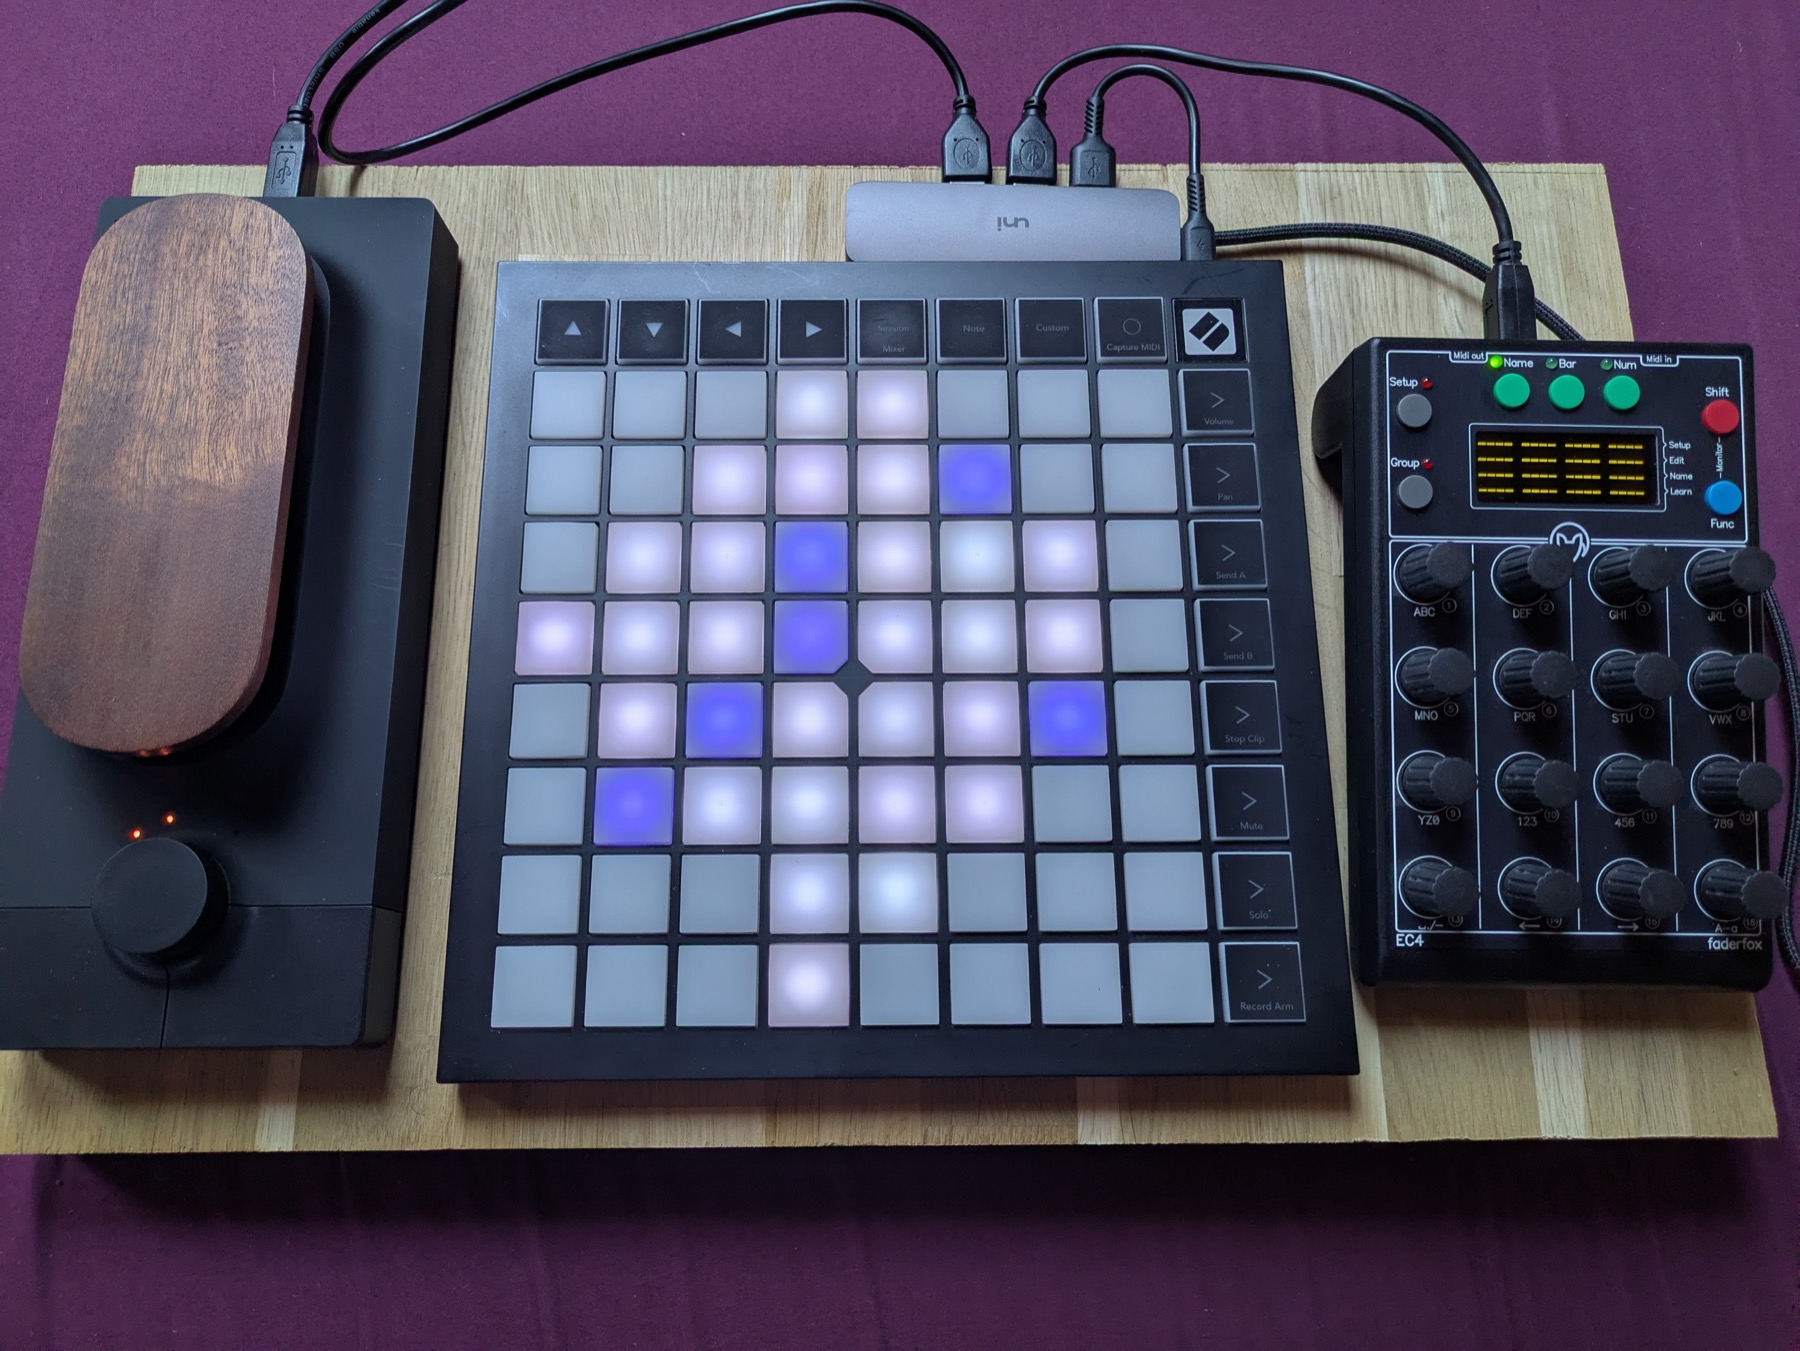
\includegraphics[width=\textwidth]{launchpad.jpg}
\caption{Launchpad set up to play the keyboard mapping of Figure
\ref{fig:dal-reduced}. Usually dustier.}
\label{fig:launchpad}
\end{figure}

The Launchpad doesn't have a mod wheel or any sliders or knobs, although its
keys can be programmed to send MIDI CC messages. So I put the Launchpad next to
an expression controller and a knob controller on a sawn-off piece of kitchen
counter, and connect them all to a USB hub (nice to have only one USB cable to
plug/unplug).

I wrote some Python scripts to apply the various kinds of keyboard mapping
described in this article on the Launchpad. I've put them in a Python package
called \texttt{gral}.\footnote{Available at
\url{https://github.com/narenratan/gral}} The README gives more details but
just to give some examples, to map Partch's scale by scale degree with $s = 2$
and $t = 7$ as in Figure \ref{fig:partch2-7} you can run
\vspace{-2ex}
\begin{verbatim}
    > scale-degree xen03-secor-partch.scl -s 2 7
\end{verbatim}
\vspace{-2ex}
where \texttt{xen03-secor-partch.scl} is an scl file containing Partch's
scale.\footnotemark{} To map Partch's scale with a harmonic template you can
run
\vspace{-2ex}
\begin{verbatim}
    > harmonic-template xen03-secor-partch.scl -t template.csv
\end{verbatim}
\vspace{-2ex}
where \texttt{template.csv} contains the harmonic template to use in table
form. The \texttt{gral} package also contains a \texttt{gral-search} program to
apply the Gral method as in Table \ref{tab:gral-25-43} and the \texttt{box-opt}
program of Section \ref{sec:box-optimization} used to find harmonic templates.
\footnotetext{scl files for many of the scales in this article can be found in
\url{https://github.com/narenratan/scale-library}}

To end roughly where we started, Figure \ref{fig:partch-launchpad} shows a
mapping of Partch's 43-tone scale which is well-suited to the Launchpad. The
middle block of the mapping fits on the Launchpad, while the 11/10 and 20/11
sadly don't. The mapping in Figure \ref{fig:partch-launchpad} is clearly
related to the mapping in Figure \ref{fig:partch-example}, in fact by a shear
to form a convenient Launchpad-sized block. Their harmonic templates are in the
same family in the sense of Appendix \ref{sec:families}.

\begin{figure}
\begin{center}
\begin{center}
$\begin{NiceArray}[first-col, last-row, columns-width=1.1cm]{|c|c|c|c|c|c|c|c|c|c|c|c|}
\hline
 &    \scriptstyle 
 &
 &    \scriptstyle 
 &    \scriptstyle 
 &    \scriptstyle 
 &    \scriptstyle 
 &\cellcolor{blue!25}     \scriptstyle 
 &
 &
 &
 &
 &
\\
5 &    20/11
 &
 &    15/8
 &    40/21
 &    64/33
 &    160/81
 &\cellcolor{blue!25}     2/1
 &
 &
 &
 &
 &
\\
 &    \scriptstyle 1035
 &
 &    \scriptstyle 1088
 &    \scriptstyle 1116
 &    \scriptstyle 1147
 &    \scriptstyle 1178
 &\cellcolor{blue!25}     \scriptstyle 1200
 &
 &
 &
 &
 &
\\
\hline
 &
 &
 &    \scriptstyle 
 &    \scriptstyle 
 &    \scriptstyle 
 &    \scriptstyle 
 &\cellcolor{blue!25}     \scriptstyle 
 &    \scriptstyle 
 &    \scriptstyle 
 &    \scriptstyle 
 &
 &
\\
4 &
 &
 &    18/11
 &    5/3
 &    27/16
 &    12/7
 &\cellcolor{blue!25}     7/4
 &    16/9
 &    9/5
 &    11/6
 &
 &
\\
 &
 &
 &    \scriptstyle 853
 &    \scriptstyle 884
 &    \scriptstyle 906
 &    \scriptstyle 933
 &\cellcolor{blue!25}     \scriptstyle 969
 &    \scriptstyle 996
 &    \scriptstyle 1018
 &    \scriptstyle 1049
 &
 &
\\
\hline
 &
 &
 &    \scriptstyle 
 &    \scriptstyle 
 &    \scriptstyle 
 &\cellcolor{blue!25}     \scriptstyle 
 &    \scriptstyle 
 &    \scriptstyle 
 &    \scriptstyle 
 &    \scriptstyle 
 &
 &
\\
3 &
 &
 &    10/7
 &    16/11
 &    40/27
 &\cellcolor{blue!25}     3/2
 &    32/21
 &    14/9
 &    11/7
 &    8/5
 &
 &
\\
 &
 &
 &    \scriptstyle 618
 &    \scriptstyle 649
 &    \scriptstyle 680
 &\cellcolor{blue!25}     \scriptstyle 702
 &    \scriptstyle 729
 &    \scriptstyle 765
 &    \scriptstyle 782
 &    \scriptstyle 814
 &
 &
\\
\hline
 &
 &
 &\cellcolor{blue!25}     \scriptstyle 
 &    \scriptstyle 
 &    \scriptstyle 
 &    \scriptstyle 
 &    \scriptstyle 
 &    \scriptstyle 
 &\cellcolor{blue!25}     \scriptstyle 
 &    \scriptstyle 
 &
 &
\\
2 &
 &
 &\cellcolor{blue!25}     5/4
 &    14/11
 &    9/7
 &    21/16
 &    4/3
 &    27/20
 &\cellcolor{blue!25}     11/8
 &    7/5
 &
 &
\\
 &
 &
 &\cellcolor{blue!25}     \scriptstyle 386
 &    \scriptstyle 418
 &    \scriptstyle 435
 &    \scriptstyle 471
 &    \scriptstyle 498
 &    \scriptstyle 520
 &\cellcolor{blue!25}     \scriptstyle 551
 &    \scriptstyle 582
 &
 &
\\
\hline
 &
 &
 &    \scriptstyle 
 &    \scriptstyle 
 &    \scriptstyle 
 &    \scriptstyle 
 &    \scriptstyle 
 &    \scriptstyle 
 &    \scriptstyle 
 &    \scriptstyle 
 &
 &
\\
1 &
 &
 &    12/11
 &    10/9
 &    9/8
 &    8/7
 &    7/6
 &    32/27
 &    6/5
 &    11/9
 &
 &
\\
 &
 &
 &    \scriptstyle 151
 &    \scriptstyle 182
 &    \scriptstyle 204
 &    \scriptstyle 231
 &    \scriptstyle 267
 &    \scriptstyle 294
 &    \scriptstyle 316
 &    \scriptstyle 347
 &
 &
\\
\hline
 &
 &
 &
 &
 &
 &\cellcolor{blue!25}     \scriptstyle 
 &    \scriptstyle 
 &    \scriptstyle 
 &    \scriptstyle 
 &    \scriptstyle 
 &
 &    \scriptstyle 
\\
0 &
 &
 &
 &
 &
 &\cellcolor{blue!25}     1/1
 &    81/80
 &    33/32
 &    21/20
 &    16/15
 &
 &    11/10
\\
 &
 &
 &
 &
 &
 &\cellcolor{blue!25}     \scriptstyle 0
 &    \scriptstyle 22
 &    \scriptstyle 53
 &    \scriptstyle 84
 &    \scriptstyle 112
 &
 &    \scriptstyle 165
\\
\hline
& -5 & -4 & -3 & -2 & -1 & 0 & 1 & 2 & 3 & 4 & 5 & 6
\end{NiceArray}$
\end{center}

\end{center}
\caption{A mapping of Partch's 43-tone scale well-suited to the Launchpad.}
\label{fig:partch-launchpad}
\end{figure}

\clearpage
\appendix

\appendixpage

\section{Wilson's method for finding harmonic templates}
\label{sec:heuristic}
Wilson gave a heuristic method for finding harmonic templates
\cite{wilsonharmonic}. The method is to pick an equal temperament $n$ and find
the equal temperament step $r$ closest in pitch to each octave-reduced harmonic
in the template. Then pick a scale degree $m$ to use as the generator and find
a chain position $p$ for each scale degree $r$ by solving
\begin{align}
    r \equiv pm \pmod{n}.
\end{align}
This is a congruence with infinitely many solutions.\footnote{The notation $a
\equiv b \pmod c$ means $a = b + kc$ for some integer $k$.} Pick the solution
$p$ with $0 \leq p < n$ and the solution $n$ below this as possible chain
positions.\footnote{The congruence can be solved using the modular inverse; in
Python \texttt{p = (pow(m, -1, n) * r) \% n}.}

For example, say we use 31TET so $n = 31$. Say we use scale step $m = 18$ as
the generator. Consider the harmonic $5/4$ in the template. Scale degree 10 in
31TET is closest in pitch to 5/4, so $r = 10$. To find possible chain positions
$p$ we need to solve $10 = 18 p \pmod{31}$, and we take the solutions $p = 4$
and $p = -27$.  Table \ref{table:template} shows the scale positions and chain
positions we get for a template containing 2/1, 3/2, 5/4, 7/4, and 11/8.

To get from a table like Table \ref{table:template} to an actual harmonic
template, we map an $m/n$ scale using the Gral method and use the scale
positions and chain positions as moduluses and chain positions on the keyboard.
So having chosen a keyboard with the Gral method, Table \ref{table:template}
gives two possible keyboard positions for each harmonic in the template,
corresponding to the two choices of chain position.

Continuing the 31TET example, applying the Gral method to 18/31 (Table
\ref{tab:gral-18-31}) we get among others the 4/7 keyboard. Figure
\ref{fig:heuristic} shows the template from Table \ref{table:template} mapped
to the 4/7 keyboard. The template we get from the positive chain positions is
shown in blue; the alternative position for 11/8 with chain position $-13$ is
shown in green. The blue harmonic template is exactly the template used in
Wilson's D'alessandro mapping (\cite{wilson1989dal}, Figure 24). The template
using the alternative position for 11/8 is the inverted D'alessandro template
(\cite{wilson1989dal}, Figure 27).

\begin{table}
\begin{center}
\begin{tabular}{cccc}
\toprule
Ratio   &   Scale position  &   \multicolumn{2}{c}{Chain positions} \\
\cmidrule{3-4}
        &                   &   Positive    &   Negative    \\
\midrule
2/1     &   31              &   0   &   $-31$   \\
3/2     &   18              &   1   &   $-30$   \\
5/4     &   10              &   4   &   $-27$   \\
7/4     &   25              &   10  &   $-21$   \\
11/8    &   14              &   18  &   $-13$   \\
\bottomrule
\end{tabular}
\end{center}
\vspace{-0.25cm}
\caption{Table of scale position and chain positions used to find harmonic
templates. This table uses a generator of 18 steps of 31TET.\vspace{0.7cm}}
\label{table:template}
\end{table}

\begin{table}
\begin{center}
\begin{tabular}{rr@{\hspace{1cm}}r@{\hspace{1cm}}rr@{\hspace{1cm}}rr@{\hspace{1cm}}rr}
\toprule
Left    &   Right   &   Mediant &   $a$  &  $b$  &  $c$  &  $d$  &  $s$  &  $t$  \\
\midrule
$0/1$ & $1/0$ & $1/1$ & $0$ & $1$ & $1$ & $0$ & $31$ & $18$ \\
      & $1/1$ & $1/2$ & $0$ & $1$ & $1$ & $1$ & $13$ & $18$ \\
$1/2$ &       & $2/3$ & $1$ & $1$ & $2$ & $1$ & $13$ & $5$ \\
      & $2/3$ & $3/5$ & $1$ & $2$ & $2$ & $3$ & $8$ & $5$ \\
      & $3/5$ & $4/7$ & $1$ & $3$ & $2$ & $5$ & $3$ & $5$ \\
$4/7$ &       & $7/12$ & $4$ & $3$ & $7$ & $5$ & $3$ & $2$ \\
      & $7/12$ & $11/19$ & $4$ & $7$ & $7$ & $12$ & $1$ & $2$ \\
$11/19$ &       & $18/31$ & $11$ & $7$ & $19$ & $12$ & $1$ & $1$ \\
\bottomrule
\end{tabular}
\end{center}
\vspace{-0.25cm}
\caption{Gral method applied to 18/31.\vspace{0.65cm}}
\label{tab:gral-18-31}
\end{table}

\begin{figure}
\begin{center}
$\begin{NiceArray}[first-col, last-row, columns-width=1.1cm]{|c|c|c|c|c|c|}
\hline
 &    \scriptstyle \scriptstyle \raisebox{.2\height}{\scalebox{.6}{+}}20\ \ \ 19.
 &    \scriptstyle \scriptstyle \raisebox{.2\height}{\scalebox{.6}{+}}15\ \ \ 22.
 &    \scriptstyle \cellcolor{blue!25}\scriptstyle \raisebox{.2\height}{\scalebox{.6}{+}}10\ \ \ 25.
 &    \scriptstyle \scriptstyle \raisebox{.2\height}{\scalebox{.6}{+}}5\ \ \ 28.
 &    \scriptstyle \cellcolor{blue!25}\scriptstyle \raisebox{.2\height}{\scalebox{.6}{+}}0\ \ \ 31.
 &    \scriptstyle \scriptstyle \raisebox{.2\height}{\scalebox{.8}{-}}5\ \ \ 34.
\\
5 &    
 &    
 &    \cellcolor{blue!25}7/4
 &    
 &    \cellcolor{blue!25}2/1
 &    
\\
 &    \scriptstyle 
 &    \scriptstyle 
 &    \scriptstyle \cellcolor{blue!25}
 &    \scriptstyle 
 &    \scriptstyle \cellcolor{blue!25}
 &    \scriptstyle 
\\
\hline
 &    \scriptstyle \cellcolor{blue!25}\scriptstyle \raisebox{.2\height}{\scalebox{.6}{+}}18\ \ \ 14.
 &    \scriptstyle \scriptstyle \raisebox{.2\height}{\scalebox{.6}{+}}13\ \ \ 17.
 &    \scriptstyle \scriptstyle \raisebox{.2\height}{\scalebox{.6}{+}}8\ \ \ 20.
 &    \scriptstyle \scriptstyle \raisebox{.2\height}{\scalebox{.6}{+}}3\ \ \ 23.
 &    \scriptstyle \scriptstyle \raisebox{.2\height}{\scalebox{.8}{-}}2\ \ \ 26.
 &    \scriptstyle \scriptstyle \raisebox{.2\height}{\scalebox{.8}{-}}7\ \ \ 29.
\\
4 &    \cellcolor{blue!25}11/8
 &    
 &    
 &    
 &    
 &    
\\
 &    \scriptstyle \cellcolor{blue!25}
 &    \scriptstyle 
 &    \scriptstyle 
 &    \scriptstyle 
 &    \scriptstyle 
 &    \scriptstyle 
\\
\hline
 &    \scriptstyle \scriptstyle \raisebox{.2\height}{\scalebox{.6}{+}}16\ \ \ 9.
 &    \scriptstyle \scriptstyle \raisebox{.2\height}{\scalebox{.6}{+}}11\ \ \ 12.
 &    \scriptstyle \scriptstyle \raisebox{.2\height}{\scalebox{.6}{+}}6\ \ \ 15.
 &    \scriptstyle \cellcolor{blue!25}\scriptstyle \raisebox{.2\height}{\scalebox{.6}{+}}1\ \ \ 18.
 &    \scriptstyle \scriptstyle \raisebox{.2\height}{\scalebox{.8}{-}}4\ \ \ 21.
 &    \scriptstyle \scriptstyle \raisebox{.2\height}{\scalebox{.8}{-}}9\ \ \ 24.
\\
3 &    
 &    
 &    
 &    \cellcolor{blue!25}3/2
 &    
 &    
\\
 &    \scriptstyle 
 &    \scriptstyle 
 &    \scriptstyle 
 &    \scriptstyle \cellcolor{blue!25}
 &    \scriptstyle 
 &    \scriptstyle 
\\
\hline
 &    \scriptstyle \scriptstyle \raisebox{.2\height}{\scalebox{.6}{+}}14\ \ \ 4.
 &    \scriptstyle \scriptstyle \raisebox{.2\height}{\scalebox{.6}{+}}9\ \ \ 7.
 &    \scriptstyle \cellcolor{blue!25}\scriptstyle \raisebox{.2\height}{\scalebox{.6}{+}}4\ \ \ 10.
 &    \scriptstyle \scriptstyle \raisebox{.2\height}{\scalebox{.8}{-}}1\ \ \ 13.
 &    \scriptstyle \scriptstyle \raisebox{.2\height}{\scalebox{.8}{-}}6\ \ \ 16.
 &    \scriptstyle \scriptstyle \raisebox{.2\height}{\scalebox{.8}{-}}11\ \ \ 19.
\\
2 &    
 &    
 &    \cellcolor{blue!25}5/4
 &    
 &    
 &    
\\
 &    \scriptstyle 
 &    \scriptstyle 
 &    \scriptstyle \cellcolor{blue!25}
 &    \scriptstyle 
 &    \scriptstyle 
 &    \scriptstyle 
\\
\hline
 &    \scriptstyle \scriptstyle \raisebox{.2\height}{\scalebox{.6}{+}}12\ \ \ \raisebox{.2\height}{\scalebox{.8}{-}}1.
 &    \scriptstyle \scriptstyle \raisebox{.2\height}{\scalebox{.6}{+}}7\ \ \ 2.
 &    \scriptstyle \scriptstyle \raisebox{.2\height}{\scalebox{.6}{+}}2\ \ \ 5.
 &    \scriptstyle \scriptstyle \raisebox{.2\height}{\scalebox{.8}{-}}3\ \ \ 8.
 &    \scriptstyle \scriptstyle \raisebox{.2\height}{\scalebox{.8}{-}}8\ \ \ 11.
 &    \scriptstyle \cellcolor{green!25}\scriptstyle \raisebox{.2\height}{\scalebox{.8}{-}}13\ \ \ 14.
\\
1 &    
 &    
 &    
 &    
 &    
 &    \cellcolor{green!25}11/8
\\
 &    \scriptstyle 
 &    \scriptstyle 
 &    \scriptstyle 
 &    \scriptstyle 
 &    \scriptstyle 
 &    \scriptstyle \cellcolor{green!25}
\\
\hline
 &    \scriptstyle \scriptstyle \raisebox{.2\height}{\scalebox{.6}{+}}10\ \ \ \raisebox{.2\height}{\scalebox{.8}{-}}6.
 &    \scriptstyle \scriptstyle \raisebox{.2\height}{\scalebox{.6}{+}}5\ \ \ \raisebox{.2\height}{\scalebox{.8}{-}}3.
 &    \scriptstyle \cellcolor{blue!25}\scriptstyle \raisebox{.2\height}{\scalebox{.6}{+}}0\ \ \ 0.
 &    \scriptstyle \scriptstyle \raisebox{.2\height}{\scalebox{.8}{-}}5\ \ \ 3.
 &    \scriptstyle \scriptstyle \raisebox{.2\height}{\scalebox{.8}{-}}10\ \ \ 6.
 &    \scriptstyle \scriptstyle \raisebox{.2\height}{\scalebox{.8}{-}}15\ \ \ 9.
\\
0 &    
 &    
 &    \cellcolor{blue!25}1/1
 &    
 &    
 &    
\\
 &    \scriptstyle 
 &    \scriptstyle 
 &    \scriptstyle \cellcolor{blue!25}
 &    \scriptstyle 
 &    \scriptstyle 
 &    \scriptstyle 
\\
\hline
& -2 & -1 & 0 & 1 & 2 & 3
\end{NiceArray}$
\end{center}

\vspace{-0.5cm}
\caption{Harmonic template from Table \ref{table:template} mapped to a 4/7
keyboard. The alternative position for 11/8 is shown in green.}
\label{fig:heuristic}
\end{figure}

\clearpage
If you already have a blank keyboard diagram labeled with chain position and
modulus (many of which are in the Wilson archive), you can immediately see
where each harmonic in Table \ref{table:template} goes on the keyboard to make
a harmonic template. You can also calculate the harmonic templates associated
with a table like Table \ref{table:template} using matrices; I think this is
useful and also sheds some light on the theory. First of all we can write Table
\ref{table:template} as a matrix $D$
\begin{align}
D   &=\matspace
\begin{bNiceMatrix}[first-row,first-col]
    &   2/1 &   3/2 &   5/4 &   7/4 &   11/8    \\
p   &   0   &   1   &   4   &   10  &   18      \\
r   &   31  &   18  &   10  &   25  &   14      \\
\end{bNiceMatrix}
\end{align}
where the first row gives chain position $p$ (here choosing the positive chain
positions) and the second row gives the modulus $r$ (taken from scale position
in the table). Then we can change from coordinates of chain position $p$ and
modulus $r$ to chain coordinates $p$ and $q$ using the matrix $N$ given by
\begin{align}
N   &=\matspace
\begin{bNiceMatrix}[first-row,first-col]
    &   p   &   q   \\
p   &   1   &   0   \\
r   &   m   &   n   \\
\end{bNiceMatrix},
\end{align}
giving a matrix $C$
\begin{align}
\label{eq:template-pq}
C   &= N^{-1} D \\
    &=\matspace
\begin{bNiceMatrix}[first-row,first-col]
    &   p   &   r   \\
p   &   1   &   0   \\
q   &   -18/31   &   1/31   \\
\end{bNiceMatrix}
\matspace
\begin{bNiceMatrix}[first-row,first-col]
    &   2/1 &   3/2 &   5/4 &   7/4 &   11/8    \\
p   &   0   &   1   &   4   &   10  &   18      \\
r   &   31  &   18  &   10  &   25  &   14      \\
\end{bNiceMatrix}
\\
    &=\matspace
\begin{bNiceMatrix}[first-row,first-col]
    &   2/1 &   3/2 &   5/4 &   7/4 &   11/8    \\
p   &   0   &   1   &   4   &   10  &   18      \\
q   &   1   &   0   &   -2  &   -5  &   -10     \\
\end{bNiceMatrix}.
\end{align}
This matrix $C$ gives the chain coordinates $p$ and $q$ for each octave reduced
harmonic. It defines a whole family of harmonic templates (see Appendix
\ref{sec:families}). To find a specific template, we use the Gral method
applied to 18/31 to choose a basis, say the basis $(1, 3)$, $(2, 5)$ for a 4/7
keyboard. We can write the basis as a matrix
\begin{align}
B   &=\matspace
\begin{bNiceMatrix}[first-row,first-col]
    &   p   &   q   \\
x   &   1   &   2   \\
y   &   3   &   5   \\
\end{bNiceMatrix}
\end{align}
and find our harmonic template $A$ as
\begin{align}
A   &=  B C \\
    &=\matspace
\begin{bNiceMatrix}[first-row,first-col]
    &   p   &   q   \\
x   &   1   &   2   \\
y   &   3   &   5   \\
\end{bNiceMatrix}
\matspace
\begin{bNiceMatrix}[first-row,first-col]
    &   2/1 &   3/2 &   5/4 &   7/4 &   11/8    \\
p   &   0   &   1   &   4   &   10  &   18      \\
q   &   1   &   0   &   -2  &   -5  &   -10     \\
\end{bNiceMatrix}
\\
    &=\matspace
\begin{bNiceMatrix}[first-row,first-col]
    &   2/1 &   3/2 &   5/4 &   7/4 &   11/8    \\
x   &   2   &   1   &   0   &   0   &   -2      \\
y   &   5   &   3   &   2   &   5   &   4       \\
\end{bNiceMatrix}
\end{align}
which gives the harmonic template shown in blue in Figure \ref{fig:heuristic}.

\section{Families of harmonic templates}
\label{sec:families}
Wilson sometimes shows keyboard mappings in related families
\cite[39-45]{wilsonhebdomekontany}, \cite[8-9]{wilsondalessandrokeyboards}.
For example, Figure \ref{fig:cinna} shows Lou Harrison's scale from Cinna
\cite{harrison1976cinna} mapped to a 3/5, 4/7, and 7/12 keyboard.  The keys are
labeled with their chain coordinates $p$ and $q$ using the basis of $3/2$ and
$2/1$.  Each note has the same chain coordinates in all three mappings. This
suggests that all three keyboard mappings can be expressed in terms of a single
mapping onto chain coordinates, and this is in fact the case.

The matrix of the harmonic template in Figure \ref{fig:cinna-3-5} is
\begin{align}
A_1 &=\matspace
\begin{bNiceMatrix}[first-row,first-col]
    &   3/2 &   2/1 &   5/4 &   7/4 \\
x   &   2   &   3   &   2   &   2   \\
y   &   1   &   2   &   0   &   2   \\
\end{bNiceMatrix},
\end{align}
for Figure \ref{fig:cinna-4-7}
\begin{align}
A_2 &=\matspace
\begin{bNiceMatrix}[first-row,first-col]
    &   3/2 &   2/1 &   5/4 &   7/4 \\
x   &   3   &   5   &   2   &   4   \\
y   &   1   &   2   &   0   &   2   \\
\end{bNiceMatrix},
\end{align}
and for Figure \ref{fig:cinna-7-12}
\begin{align}
A_3 &=\matspace
\begin{bNiceMatrix}[first-row,first-col]
    &   3/2 &   2/1 &   5/4 &   7/4 \\
x   &   4   &   7   &   2   &   6   \\
y   &   3   &   5   &   2   &   4   \\
\end{bNiceMatrix}.
\end{align}
Looking at Figure \ref{fig:cinna-3-5}, the 3/2 and 2/1 form a basis of $(a, b)
= (2, 1)$, $(c, d) = (3, 2)$. Collecting these into a matrix we can write this
basis as
\begin{align}
B_1 &=\matspace
\begin{bNiceMatrix}[first-row,first-col]
    &   p   &   q   \\
x   &   2   &   3   \\
y   &   1   &   2   \\
\end{bNiceMatrix},
\end{align}
and likewise for Figure \ref{fig:cinna-4-7} and Figure \ref{fig:cinna-7-12} we
have
\begin{align}
B_2 &=\matspace
\begin{bNiceMatrix}[first-row,first-col]
    &   p   &   q   \\
x   &   3   &   5   \\
y   &   1   &   2   \\
\end{bNiceMatrix} \\
B_3 &=\matspace
\begin{bNiceMatrix}[first-row,first-col]
    &   p   &   q   \\
x   &   4   &   7   \\
y   &   3   &   5   \\
\end{bNiceMatrix}.
\end{align}
Now putting $C = (B_1)^{-1} A_1$ we have
\begin{align}
C &=\matspace
\begin{bNiceMatrix}[first-row,first-col]
    &   3/2 &   2/1 &   5/4 &   7/4 \\
p   &   1   &   0   &   4   &   -2  \\
q   &   0   &   1   &   -2  &   2   \\
\end{bNiceMatrix}
\end{align}
and $A_1 = B_1 C$.  The nice thing is that we can use the same $C$ to write
$A_2 = B_2 C$ and $A_3 = B_3 C$.  So you might say that the matrix $C$
expresses the core of this family of keyboard mappings, and that $A_1$, $A_2$,
and $A_3$ are different manifestations of the same underlying logic --- a logic
based on chain coordinates.

So let's say that two harmonic templates $A$ and $A'$ are in the same family
whenever we can write $A = B C$ and $A' = B' C$ for some matrix $C$, where $B$
and $B'$ both have determinant $\pm1$. The interpretation is that $C$ maps the
octave-reduced harmonics onto chain coordinates $pq$, and $B$ and $B'$ are
different keyboard bases. All the harmonic templates in Figure \ref{fig:cinna}
are in the same family.

\begin{figure}
\begin{subfigure}{\textwidth}
\input{xen05-harrison-cinna-3-5.tex}
\caption{Flipped 3/5 keyboard}
\label{fig:cinna-3-5}
\par\bigskip
\end{subfigure}
\begin{subfigure}{\textwidth}
\begin{center}
$\begin{NiceArray}[first-col, last-row, columns-width=1.3cm]{|c|c|c|c|c|c|c|c|c|}
\hline
 &\scriptstyle \raisebox{.2\height}{\scalebox{.8}{-}}12\ \ \ \raisebox{.2\height}{\scalebox{.6}{+}}7
 &\scriptstyle \raisebox{.2\height}{\scalebox{.8}{-}}10\ \ \ \raisebox{.2\height}{\scalebox{.6}{+}}6
 &\scriptstyle \raisebox{.2\height}{\scalebox{.8}{-}}8\ \ \ \raisebox{.2\height}{\scalebox{.6}{+}}5
 &\scriptstyle \raisebox{.2\height}{\scalebox{.8}{-}}6\ \ \ \raisebox{.2\height}{\scalebox{.6}{+}}4
 &\scriptstyle \raisebox{.2\height}{\scalebox{.8}{-}}4\ \ \ \raisebox{.2\height}{\scalebox{.6}{+}}3
 &\cellcolor{blue!25} \scriptstyle \raisebox{.2\height}{\scalebox{.8}{-}}2\ \ \ \raisebox{.2\height}{\scalebox{.6}{+}}2
 &\cellcolor{blue!25} \scriptstyle \raisebox{.2\height}{\scalebox{.6}{+}}0\ \ \ \raisebox{.2\height}{\scalebox{.6}{+}}1
 &\scriptstyle \raisebox{.2\height}{\scalebox{.6}{+}}2\ \ \ \raisebox{.2\height}{\scalebox{.6}{+}}0
 &\scriptstyle \raisebox{.2\height}{\scalebox{.6}{+}}4\ \ \ \raisebox{.2\height}{\scalebox{.8}{-}}1
\\
2 &
 &
 &
 &
 &    8/5
 &\cellcolor{blue!25}     7/4
 &\cellcolor{blue!25}     2/1
 &
 &
\\
 &
 &
 &
 &
 &    \scriptstyle 814
 &\cellcolor{blue!25}     \scriptstyle 969
 &\cellcolor{blue!25}     \scriptstyle 1200
 &
 &
\\
\hline
 &\scriptstyle \raisebox{.2\height}{\scalebox{.8}{-}}7\ \ \ \raisebox{.2\height}{\scalebox{.6}{+}}4
 &\scriptstyle \raisebox{.2\height}{\scalebox{.8}{-}}5\ \ \ \raisebox{.2\height}{\scalebox{.6}{+}}3
 &\scriptstyle \raisebox{.2\height}{\scalebox{.8}{-}}3\ \ \ \raisebox{.2\height}{\scalebox{.6}{+}}2
 &\scriptstyle \raisebox{.2\height}{\scalebox{.8}{-}}1\ \ \ \raisebox{.2\height}{\scalebox{.6}{+}}1
 &\cellcolor{blue!25} \scriptstyle \raisebox{.2\height}{\scalebox{.6}{+}}1\ \ \ \raisebox{.2\height}{\scalebox{.6}{+}}0
 &\scriptstyle \raisebox{.2\height}{\scalebox{.6}{+}}3\ \ \ \raisebox{.2\height}{\scalebox{.8}{-}}1
 &\scriptstyle \raisebox{.2\height}{\scalebox{.6}{+}}5\ \ \ \raisebox{.2\height}{\scalebox{.8}{-}}2
 &\scriptstyle \raisebox{.2\height}{\scalebox{.6}{+}}7\ \ \ \raisebox{.2\height}{\scalebox{.8}{-}}3
 &\scriptstyle \raisebox{.2\height}{\scalebox{.6}{+}}9\ \ \ \raisebox{.2\height}{\scalebox{.8}{-}}4
\\
1 &
 &    16/15
 &    7/6
 &    4/3
 &\cellcolor{blue!25}     3/2
 &    5/3
 &    15/8
 &
 &
\\
 &
 &    \scriptstyle 112
 &    \scriptstyle 267
 &    \scriptstyle 498
 &\cellcolor{blue!25}     \scriptstyle 702
 &    \scriptstyle 884
 &    \scriptstyle 1088
 &
 &
\\
\hline
 &\scriptstyle \raisebox{.2\height}{\scalebox{.8}{-}}2\ \ \ \raisebox{.2\height}{\scalebox{.6}{+}}1
 &\cellcolor{blue!25} \scriptstyle \raisebox{.2\height}{\scalebox{.6}{+}}0\ \ \ \raisebox{.2\height}{\scalebox{.6}{+}}0
 &\scriptstyle \raisebox{.2\height}{\scalebox{.6}{+}}2\ \ \ \raisebox{.2\height}{\scalebox{.8}{-}}1
 &\cellcolor{blue!25} \scriptstyle \raisebox{.2\height}{\scalebox{.6}{+}}4\ \ \ \raisebox{.2\height}{\scalebox{.8}{-}}2
 &\scriptstyle \raisebox{.2\height}{\scalebox{.6}{+}}6\ \ \ \raisebox{.2\height}{\scalebox{.8}{-}}3
 &\scriptstyle \raisebox{.2\height}{\scalebox{.6}{+}}8\ \ \ \raisebox{.2\height}{\scalebox{.8}{-}}4
 &\scriptstyle \raisebox{.2\height}{\scalebox{.6}{+}}10\ \ \ \raisebox{.2\height}{\scalebox{.8}{-}}5
 &\scriptstyle \raisebox{.2\height}{\scalebox{.6}{+}}12\ \ \ \raisebox{.2\height}{\scalebox{.8}{-}}6
 &\scriptstyle \raisebox{.2\height}{\scalebox{.6}{+}}14\ \ \ \raisebox{.2\height}{\scalebox{.8}{-}}7
\\
0 &
 &\cellcolor{blue!25}     1/1
 &    10/9
 &\cellcolor{blue!25}     5/4
 &    25/18
 &
 &
 &
 &
\\
 &
 &\cellcolor{blue!25}     \scriptstyle 0
 &    \scriptstyle 182
 &\cellcolor{blue!25}     \scriptstyle 386
 &    \scriptstyle 569
 &
 &
 &
 &
\\
\hline
& -1 & 0 & 1 & 2 & 3 & 4 & 5 & 6 & 7
\end{NiceArray}$
\end{center}

\caption{Flipped 4/7 keyboard}
\label{fig:cinna-4-7}
\par\bigskip
\end{subfigure}
\begin{subfigure}{\textwidth}
\begin{center}
$\begin{NiceArray}[first-col, last-row, columns-width=1.3cm]{|c|c|c|c|c|c|c|c|c|}
\hline
 &\scriptstyle \raisebox{.2\height}{\scalebox{.6}{+}}40\ \ \ \raisebox{.2\height}{\scalebox{.8}{-}}23
 &\scriptstyle \raisebox{.2\height}{\scalebox{.6}{+}}35\ \ \ \raisebox{.2\height}{\scalebox{.8}{-}}20
 &\scriptstyle \raisebox{.2\height}{\scalebox{.6}{+}}30\ \ \ \raisebox{.2\height}{\scalebox{.8}{-}}17
 &\scriptstyle \raisebox{.2\height}{\scalebox{.6}{+}}25\ \ \ \raisebox{.2\height}{\scalebox{.8}{-}}14
 &\scriptstyle \raisebox{.2\height}{\scalebox{.6}{+}}20\ \ \ \raisebox{.2\height}{\scalebox{.8}{-}}11
 &\scriptstyle \raisebox{.2\height}{\scalebox{.6}{+}}15\ \ \ \raisebox{.2\height}{\scalebox{.8}{-}}8
 &\scriptstyle \raisebox{.2\height}{\scalebox{.6}{+}}10\ \ \ \raisebox{.2\height}{\scalebox{.8}{-}}5
 &\scriptstyle \raisebox{.2\height}{\scalebox{.6}{+}}5\ \ \ \raisebox{.2\height}{\scalebox{.8}{-}}2
 &\cellcolor{blue!25} \scriptstyle \raisebox{.2\height}{\scalebox{.6}{+}}0\ \ \ \raisebox{.2\height}{\scalebox{.6}{+}}1
\\
5 &
 &
 &
 &
 &
 &
 &
 &    15/8
 &\cellcolor{blue!25}     2/1
\\
 &
 &
 &
 &
 &
 &
 &
 &    \scriptstyle 1088
 &\cellcolor{blue!25}     \scriptstyle 1200
\\
\hline
 &\scriptstyle \raisebox{.2\height}{\scalebox{.6}{+}}33\ \ \ \raisebox{.2\height}{\scalebox{.8}{-}}19
 &\scriptstyle \raisebox{.2\height}{\scalebox{.6}{+}}28\ \ \ \raisebox{.2\height}{\scalebox{.8}{-}}16
 &\scriptstyle \raisebox{.2\height}{\scalebox{.6}{+}}23\ \ \ \raisebox{.2\height}{\scalebox{.8}{-}}13
 &\scriptstyle \raisebox{.2\height}{\scalebox{.6}{+}}18\ \ \ \raisebox{.2\height}{\scalebox{.8}{-}}10
 &\scriptstyle \raisebox{.2\height}{\scalebox{.6}{+}}13\ \ \ \raisebox{.2\height}{\scalebox{.8}{-}}7
 &\scriptstyle \raisebox{.2\height}{\scalebox{.6}{+}}8\ \ \ \raisebox{.2\height}{\scalebox{.8}{-}}4
 &\scriptstyle \raisebox{.2\height}{\scalebox{.6}{+}}3\ \ \ \raisebox{.2\height}{\scalebox{.8}{-}}1
 &\cellcolor{blue!25} \scriptstyle \raisebox{.2\height}{\scalebox{.8}{-}}2\ \ \ \raisebox{.2\height}{\scalebox{.6}{+}}2
 &\scriptstyle \raisebox{.2\height}{\scalebox{.8}{-}}7\ \ \ \raisebox{.2\height}{\scalebox{.6}{+}}5
\\
4 &
 &
 &
 &
 &
 &
 &    5/3
 &\cellcolor{blue!25}     7/4
 &
\\
 &
 &
 &
 &
 &
 &
 &    \scriptstyle 884
 &\cellcolor{blue!25}     \scriptstyle 969
 &
\\
\hline
 &\scriptstyle \raisebox{.2\height}{\scalebox{.6}{+}}26\ \ \ \raisebox{.2\height}{\scalebox{.8}{-}}15
 &\scriptstyle \raisebox{.2\height}{\scalebox{.6}{+}}21\ \ \ \raisebox{.2\height}{\scalebox{.8}{-}}12
 &\scriptstyle \raisebox{.2\height}{\scalebox{.6}{+}}16\ \ \ \raisebox{.2\height}{\scalebox{.8}{-}}9
 &\scriptstyle \raisebox{.2\height}{\scalebox{.6}{+}}11\ \ \ \raisebox{.2\height}{\scalebox{.8}{-}}6
 &\scriptstyle \raisebox{.2\height}{\scalebox{.6}{+}}6\ \ \ \raisebox{.2\height}{\scalebox{.8}{-}}3
 &\cellcolor{blue!25} \scriptstyle \raisebox{.2\height}{\scalebox{.6}{+}}1\ \ \ \raisebox{.2\height}{\scalebox{.6}{+}}0
 &\scriptstyle \raisebox{.2\height}{\scalebox{.8}{-}}4\ \ \ \raisebox{.2\height}{\scalebox{.6}{+}}3
 &\scriptstyle \raisebox{.2\height}{\scalebox{.8}{-}}9\ \ \ \raisebox{.2\height}{\scalebox{.6}{+}}6
 &\scriptstyle \raisebox{.2\height}{\scalebox{.8}{-}}14\ \ \ \raisebox{.2\height}{\scalebox{.6}{+}}9
\\
3 &
 &
 &
 &
 &    25/18
 &\cellcolor{blue!25}     3/2
 &    8/5
 &
 &
\\
 &
 &
 &
 &
 &    \scriptstyle 569
 &\cellcolor{blue!25}     \scriptstyle 702
 &    \scriptstyle 814
 &
 &
\\
\hline
 &\scriptstyle \raisebox{.2\height}{\scalebox{.6}{+}}19\ \ \ \raisebox{.2\height}{\scalebox{.8}{-}}11
 &\scriptstyle \raisebox{.2\height}{\scalebox{.6}{+}}14\ \ \ \raisebox{.2\height}{\scalebox{.8}{-}}8
 &\scriptstyle \raisebox{.2\height}{\scalebox{.6}{+}}9\ \ \ \raisebox{.2\height}{\scalebox{.8}{-}}5
 &\cellcolor{blue!25} \scriptstyle \raisebox{.2\height}{\scalebox{.6}{+}}4\ \ \ \raisebox{.2\height}{\scalebox{.8}{-}}2
 &\scriptstyle \raisebox{.2\height}{\scalebox{.8}{-}}1\ \ \ \raisebox{.2\height}{\scalebox{.6}{+}}1
 &\scriptstyle \raisebox{.2\height}{\scalebox{.8}{-}}6\ \ \ \raisebox{.2\height}{\scalebox{.6}{+}}4
 &\scriptstyle \raisebox{.2\height}{\scalebox{.8}{-}}11\ \ \ \raisebox{.2\height}{\scalebox{.6}{+}}7
 &\scriptstyle \raisebox{.2\height}{\scalebox{.8}{-}}16\ \ \ \raisebox{.2\height}{\scalebox{.6}{+}}10
 &\scriptstyle \raisebox{.2\height}{\scalebox{.8}{-}}21\ \ \ \raisebox{.2\height}{\scalebox{.6}{+}}13
\\
2 &
 &
 &
 &\cellcolor{blue!25}     5/4
 &    4/3
 &
 &
 &
 &
\\
 &
 &
 &
 &\cellcolor{blue!25}     \scriptstyle 386
 &    \scriptstyle 498
 &
 &
 &
 &
\\
\hline
 &\scriptstyle \raisebox{.2\height}{\scalebox{.6}{+}}12\ \ \ \raisebox{.2\height}{\scalebox{.8}{-}}7
 &\scriptstyle \raisebox{.2\height}{\scalebox{.6}{+}}7\ \ \ \raisebox{.2\height}{\scalebox{.8}{-}}4
 &\scriptstyle \raisebox{.2\height}{\scalebox{.6}{+}}2\ \ \ \raisebox{.2\height}{\scalebox{.8}{-}}1
 &\scriptstyle \raisebox{.2\height}{\scalebox{.8}{-}}3\ \ \ \raisebox{.2\height}{\scalebox{.6}{+}}2
 &\scriptstyle \raisebox{.2\height}{\scalebox{.8}{-}}8\ \ \ \raisebox{.2\height}{\scalebox{.6}{+}}5
 &\scriptstyle \raisebox{.2\height}{\scalebox{.8}{-}}13\ \ \ \raisebox{.2\height}{\scalebox{.6}{+}}8
 &\scriptstyle \raisebox{.2\height}{\scalebox{.8}{-}}18\ \ \ \raisebox{.2\height}{\scalebox{.6}{+}}11
 &\scriptstyle \raisebox{.2\height}{\scalebox{.8}{-}}23\ \ \ \raisebox{.2\height}{\scalebox{.6}{+}}14
 &\scriptstyle \raisebox{.2\height}{\scalebox{.8}{-}}28\ \ \ \raisebox{.2\height}{\scalebox{.6}{+}}17
\\
1 &
 &
 &    10/9
 &    7/6
 &
 &
 &
 &
 &
\\
 &
 &
 &    \scriptstyle 182
 &    \scriptstyle 267
 &
 &
 &
 &
 &
\\
\hline
 &\scriptstyle \raisebox{.2\height}{\scalebox{.6}{+}}5\ \ \ \raisebox{.2\height}{\scalebox{.8}{-}}3
 &\cellcolor{blue!25} \scriptstyle \raisebox{.2\height}{\scalebox{.6}{+}}0\ \ \ \raisebox{.2\height}{\scalebox{.6}{+}}0
 &\scriptstyle \raisebox{.2\height}{\scalebox{.8}{-}}5\ \ \ \raisebox{.2\height}{\scalebox{.6}{+}}3
 &\scriptstyle \raisebox{.2\height}{\scalebox{.8}{-}}10\ \ \ \raisebox{.2\height}{\scalebox{.6}{+}}6
 &\scriptstyle \raisebox{.2\height}{\scalebox{.8}{-}}15\ \ \ \raisebox{.2\height}{\scalebox{.6}{+}}9
 &\scriptstyle \raisebox{.2\height}{\scalebox{.8}{-}}20\ \ \ \raisebox{.2\height}{\scalebox{.6}{+}}12
 &\scriptstyle \raisebox{.2\height}{\scalebox{.8}{-}}25\ \ \ \raisebox{.2\height}{\scalebox{.6}{+}}15
 &\scriptstyle \raisebox{.2\height}{\scalebox{.8}{-}}30\ \ \ \raisebox{.2\height}{\scalebox{.6}{+}}18
 &\scriptstyle \raisebox{.2\height}{\scalebox{.8}{-}}35\ \ \ \raisebox{.2\height}{\scalebox{.6}{+}}21
\\
0 &
 &\cellcolor{blue!25}     1/1
 &    16/15
 &
 &
 &
 &
 &
 &
\\
 &
 &\cellcolor{blue!25}     \scriptstyle 0
 &    \scriptstyle 112
 &
 &
 &
 &
 &
 &
\\
\hline
& -1 & 0 & 1 & 2 & 3 & 4 & 5 & 6 & 7
\end{NiceArray}$
\end{center}

\caption{7/12 keyboard}
\label{fig:cinna-7-12}
\par\bigskip
\end{subfigure}
\caption{A family of keyboard mappings for Lou Harrison's scale from Cinna.}
\label{fig:cinna}
\end{figure}

\begin{figure}
\begin{subfigure}{\textwidth}
\input{xen05-harrison-cinna-a.tex}
\caption{Flipped 3/5 keyboard, compare Figure \ref{fig:cinna-3-5}.}
\label{fig:cinna-2-1}
\par\bigskip
\end{subfigure}
\begin{subfigure}{\textwidth}
\begin{center}
$\begin{NiceArray}[first-col, last-row, columns-width=1.3cm]{|c|c|c|c|c|c|c|c|c|}
\hline
 &
 &
 &\cellcolor{blue!25}     \scriptstyle 
 &    \scriptstyle 
 &\cellcolor{blue!25}     \scriptstyle 
 &
 &
 &
 &
\\
3 &
 &
 &\cellcolor{blue!25}     7/4
 &    15/8
 &\cellcolor{blue!25}     2/1
 &
 &
 &
 &
\\
 &
 &
 &\cellcolor{blue!25}     \scriptstyle 969
 &    \scriptstyle 1088
 &\cellcolor{blue!25}     \scriptstyle 1200
 &
 &
 &
 &
\\
\hline
 &
 &
 &\cellcolor{blue!25}     \scriptstyle 
 &    \scriptstyle 
 &    \scriptstyle 
 &
 &
 &
 &
\\
2 &
 &
 &\cellcolor{blue!25}     3/2
 &    8/5
 &    5/3
 &
 &
 &
 &
\\
 &
 &
 &\cellcolor{blue!25}     \scriptstyle 702
 &    \scriptstyle 814
 &    \scriptstyle 884
 &
 &
 &
 &
\\
\hline
 &
 &    \scriptstyle 
 &\cellcolor{blue!25}     \scriptstyle 
 &    \scriptstyle 
 &    \scriptstyle 
 &
 &
 &
 &
\\
1 &
 &    7/6
 &\cellcolor{blue!25}     5/4
 &    4/3
 &    25/18
 &
 &
 &
 &
\\
 &
 &    \scriptstyle 267
 &\cellcolor{blue!25}     \scriptstyle 386
 &    \scriptstyle 498
 &    \scriptstyle 569
 &
 &
 &
 &
\\
\hline
 &
 &\cellcolor{blue!25}     \scriptstyle 
 &    \scriptstyle 
 &    \scriptstyle 
 &
 &
 &
 &
 &
\\
0 &
 &\cellcolor{blue!25}     1/1
 &    16/15
 &    10/9
 &
 &
 &
 &
 &
\\
 &
 &\cellcolor{blue!25}     \scriptstyle 0
 &    \scriptstyle 112
 &    \scriptstyle 182
 &
 &
 &
 &
 &
\\
\hline
& -1 & 0 & 1 & 2 & 3 & 4 & 5 & 6 & 7
\end{NiceArray}$
\end{center}

\caption{Mapping in which 3/2 and 2/1 don't form a basis.}
\label{fig:cinna-2-2}
\par\bigskip
\end{subfigure}
\caption{Harmonic templates not in the family of Figure \ref{fig:cinna}}
\label{fig:cinna-2}
\end{figure}

Figure \ref{fig:cinna-2} shows two harmonic templates which aren't in the same
family as the Figure \ref{fig:cinna} templates. The harmonic template for
Figure \ref{fig:cinna-2-1} is
\begin{align}
A_4 &=\matspace
\begin{bNiceMatrix}[first-row,first-col]
    &   3/2 &   2/1 &   5/4 &   7/4 \\
x   &   2   &   3   &   0   &   4   \\
y   &   1   &   2   &   1   &   1   \\
\end{bNiceMatrix}
\end{align}
and for Figure \ref{fig:cinna-2-2} we have
\begin{align}
A_5 &=\matspace
\begin{bNiceMatrix}[first-row,first-col]
    &   3/2 &   2/1 &   5/4 &   7/4 \\
x   &   1   &   3   &   1   &   1   \\
y   &   2   &   3   &   1   &   3   \\
\end{bNiceMatrix}.
\end{align}
But how do we know that $A_4$ and $A_5$ aren't in the same family as the Figure
\ref{fig:cinna} templates? It turns out that two harmonic templates are in the
same family if and only if their Hermite normal forms
\cite{schrijver1998theory, newman1972integral} are the same.\footnote{If $A$
and $A'$ are in the same family, $A = BC$ and $A' = B'C$,
so $A' = B' B^{-1} A$. Since $B$ and $B'$ are unimodular (i.e. have determinant
$\pm1$), $B' B^{-1}$ is unimodular. Multiplying a matrix by a unimodular matrix
doesn't change its Hermite normal form, so $A$ and $A'$ have the same Hermite
normal form.  Going the other way, if $A$ and $A'$ have the same Hermite normal
form $H$, then $A = UH$ and $A' = U'H$ for some unimodular $U$ and $U'$, so $A$
and $A'$ are in the same family.
} Table \ref{tab:hermite} shows the harmonic templates of Figure
\ref{fig:cinna} and Figure \ref{fig:cinna-2} together with their Hermite normal
forms. You can see that $A_1$, $A_2$, and $A_3$ all have the same Hermite
normal form, while $A_4$ and $A_5$ have different ones. Looking at the $(1, 0)$
and $(0, 1)$ columns in the Hermite normal forms, you can also see that 3/2 and
2/1 form a basis for $A_1$, $A_2$, $A_3$, and $A_4$, while 5/4 and 3/2 form a
basis for $A_5$.

Wilson's heuristic for producing harmonic templates \cite{wilsonharmonic},
compare \cite[38]{wilsonhebdomekontany}, gives them in coordinates of chain
position $p$ and modulus $r$ (see Appendix \ref{sec:heuristic}). These can
immediately be transformed to chain coordinates $p$ and $q$ (Equation
\ref{eq:template-pq}) and so give rise to a family of harmonic templates
related in the sense of this appendix.

\addtolength{\tabcolsep}{10pt}
\begin{table}
\centering
\begin{tabular}{c c c}
    &   Matrix  &   Hermite normal form
\par\medskip
\\
$A_1$
&
$
\begin{bNiceMatrix}[first-row,first-col]
    &   3/2 &   2/1 &   5/4 &   7/4 \\
x   &   2   &   3   &   2   &   2   \\
y   &   1   &   2   &   0   &   2   \\
\end{bNiceMatrix}
$
&
$
\begin{bNiceMatrix}[first-row,first-col]
    &   3/2 &   2/1 &   5/4 &   7/4 \\
p   &   1   &   0   &   4   &   -2  \\
q   &   0   &   1   &   -2  &   2   \\
\end{bNiceMatrix}
$
\par\bigskip
\\
$A_2$
&
$
\begin{bNiceMatrix}[first-row,first-col]
    &   3/2 &   2/1 &   5/4 &   7/4 \\
x   &   3   &   5   &   2   &   4   \\
y   &   1   &   2   &   0   &   2   \\
\end{bNiceMatrix}
$
&
$
\begin{bNiceMatrix}[first-row,first-col]
    &   3/2 &   2/1 &   5/4 &   7/4 \\
p   &   1   &   0   &   4   &   -2  \\
q   &   0   &   1   &   -2  &   2   \\
\end{bNiceMatrix}
$
\par\bigskip
\\
$A_3$
&
$
\begin{bNiceMatrix}[first-row,first-col]
    &   3/2 &   2/1 &   5/4 &   7/4 \\
x   &   4   &   7   &   2   &   6   \\
y   &   3   &   5   &   2   &   4   \\
\end{bNiceMatrix}
$
&
$
\begin{bNiceMatrix}[first-row,first-col]
    &   3/2 &   2/1 &   5/4 &   7/4 \\
p   &   1   &   0   &   4   &   -2  \\
q   &   0   &   1   &   -2  &   2   \\
\end{bNiceMatrix}
$
\par\bigskip
\\
$A_4$
&
$
\begin{bNiceMatrix}[first-row,first-col]
    &   3/2 &   2/1 &   5/4 &   7/4 \\
x   &   2   &   3   &   0   &   4   \\
y   &   1   &   2   &   1   &   1   \\
\end{bNiceMatrix}
$
&
$
\begin{bNiceMatrix}[first-row,first-col]
    &   3/2 &   2/1 &   5/4 &   7/4 \\
p   &   1   &   0   &   -3  &   5   \\
q   &   0   &   1   &   2   &   -2  \\
\end{bNiceMatrix}
$
\par\bigskip
\\
$A_5$
&
$
\begin{bNiceMatrix}[first-row,first-col]
    &   3/2 &   2/1 &   5/4 &   7/4 \\
x   &   1   &   3   &   1   &   1   \\
y   &   2   &   3   &   1   &   3   \\
\end{bNiceMatrix}
$
&
$
\begin{bNiceMatrix}[first-row,first-col]
    &   3/2 &   2/1 &   5/4 &   7/4 \\
p   &   1   &   0   &   0   &   2   \\
q   &   0   &   3   &   1   &   -1  \\
\end{bNiceMatrix}
$
\par\bigskip
\\
\end{tabular}
\caption{Table of harmonic templates of Figure \ref{fig:cinna} and Figure
\ref{fig:cinna-2} with their Hermite normal forms.}
\label{tab:hermite}
\end{table}
\addtolength{\tabcolsep}{-10pt}

\clearpage
\section{The Gral method and moments of symmetry}
It's surprising that the Gral method, apparently about lattice bases, can
calculate moments of symmetry (see Section \ref{subsec:relation}). This
appendix uses keyboard mapping to give some intuition for this and to derive
some useful formulae.

Given a basis $(a, b)$, $(c, d)$ we can find chain coordinates $(p, q)$ for
every key $(x, y)$ on the keyboard according to
\begin{align}
\begin{bmatrix}
    p \\
    q \\
\end{bmatrix}
    &=
\frac{1}{\Delta}
\begin{bmatrix}
    d & -c \\
    -b & a \\
\end{bmatrix}
\begin{bmatrix}
    x \\
    y \\
\end{bmatrix}
\end{align}
where $\Delta = ad - bc = \pm 1$. If we're stacking a generator at $(a, b)$
with pitch $g$ cents within a period at $(c, d)$ with pitch $h$ cents, we can
assign a pitch $u$ to any key as $u = pg + qh$. Figure \ref{fig:stack} shows
the pitches we get in this way when using a basis $(1, 3)$, $(2, 5)$ and
stacking a generator $g = 707$ cents within a period $h = 1200$ cents.

\begin{figure}
\begin{center}
\input{stack.tex}
\end{center}
\caption{Pitches determined by chain coordinates when stacking a generator of
707 cents.}
\label{fig:stack}
\end{figure}

\clearpage
The pitches from stacking always increase by the same amount $\sigma$ going
along a row or $\tau$ going up a column; in Figure \ref{fig:stack}, $\sigma =
65$ cents and $\tau = 214$ cents. We can derive expressions for $\sigma$ and
$\tau$ from the pitch $u$ as follows:
\begin{align}
u   &= p g + q h    \\
    &=
\begin{bmatrix}
    g   &   h   \\
\end{bmatrix}
\begin{bmatrix}
    p   \\
    q   \\
\end{bmatrix}   \\
    &=
\begin{bmatrix}
    g   &   h   \\
\end{bmatrix}
\frac{1}{\Delta}
\begin{bmatrix}
    d & -c \\
    -b & a \\
\end{bmatrix}
\begin{bmatrix}
    x \\
    y \\
\end{bmatrix}   \\
    &=
\frac{1}{\Delta}
\begin{bmatrix}
    d g - b h   &   -c g + a h  \\
\end{bmatrix}
\begin{bmatrix}
    x \\
    y \\
\end{bmatrix}   \\
    &=
\begin{bmatrix}
    \sigma  &   \tau   \\
\end{bmatrix}
\begin{bmatrix}
    x \\
    y \\
\end{bmatrix}
\end{align}
where
\begin{align}
    \sigma  &=  \frac{d g - b h}{\Delta}    \label{eq:mos-step-sizes-1}\\
    \tau    &=  \frac{-c g + a h}{\Delta}.  \label{eq:mos-step-sizes-2}
\end{align}
Checking the example from Figure \ref{fig:stack} we get $\sigma = (5 \cdot 707
- 3 \cdot 1200)/{-1} = 65$ and $\tau = (-2 \cdot 707 + 1 \cdot 1200)/{-1} =
214$, the correct values.

If we want the pitch to increase going along each row and up each column, our
choice of basis is constrained --- we need $\sigma > 0$ and $\tau > 0$,
that is
\begin{align}
    \frac{d g - b h}{\Delta}    &   > 0 \\
    \frac{-c g + a h}{\Delta}   &   > 0.
\end{align}
If $\Delta = -1$ and $c > 0$, $d > 0$, we can write these conditions as
\begin{align}
    \frac{a}{c} < \frac{g}{h} < \frac{b}{d}.
\label{eq:positive-stack}
\end{align}
This is analogous to the condition in Equation \ref{eq:positive-special} when
mapping a scale by scale degree, and here also the Gral method gives all bases
with $\Delta = -1$ and non-negative coordinates which satisfy Equation
\ref{eq:positive-stack}. The method is the same as in Section
\ref{sec:scale-degree-mapping}, a binary search for $g/h$ using the mediant to
bisect the search interval, except in general $g/h$ can be an irrational number
in which case the search goes on indefinitely. Table \ref{tab:gral-mos} shows
the Gral method applied to $g/h = 707/1200$.  Each row shows the left and right
endpoints of the search interval, their mediant, the corresponding basis $(a,
b)$, $(c, d)$, and the resulting step sizes $\sigma$ and $\tau$. The mapping in
Figure \ref{fig:stack} comes from the row with mediant 4/7.

\begin{table}
\centering
\begin{tabular}{rr@{\hspace{1cm}}r@{\hspace{1cm}}rr@{\hspace{1cm}}rr@{\hspace{1cm}}rr}
\toprule
Left    &   Right   &   Mediant &   $a$  &  $b$  &  $c$  &  $d$  &  $\sigma$  &  $\tau$  \\
\midrule
$0/1$ & $1/0$ & $1/1$ & $0$ & $1$ & $1$ & $0$ & $1200$ & $707$ \\
      & $1/1$ & $1/2$ & $0$ & $1$ & $1$ & $1$ & $493$ & $707$ \\
$1/2$ &       & $2/3$ & $1$ & $1$ & $2$ & $1$ & $493$ & $214$ \\
      & $2/3$ & $3/5$ & $1$ & $2$ & $2$ & $3$ & $279$ & $214$ \\
      & $3/5$ & $4/7$ & $1$ & $3$ & $2$ & $5$ & $65$ & $214$ \\
$4/7$ &       & $7/12$ & $4$ & $3$ & $7$ & $5$ & $65$ & $149$ \\
$7/12$ &       & $10/17$ & $7$ & $3$ & $12$ & $5$ & $65$ & $84$ \\
$10/17$ &       & $13/22$ & $10$ & $3$ & $17$ & $5$ & $65$ & $19$ \\
      & $13/22$ & $23/39$ & $10$ & $13$ & $17$ & $22$ & $46$ & $19$ \\
$\vdots\quad$ & $\vdots\quad$ & $\vdots\quad$ & $\vdots\;$ & $\vdots\;$ & $\vdots\;$ & $\vdots\;$ & $\vdots\;$ & $\vdots\;$ \\
\bottomrule
\end{tabular}
\caption{Table showing the Gral method applied to $g/h = 707/1200$.}
\label{tab:gral-mos}
\end{table}

A basis gives us a keyboard mapping of the infinite collection of pitches $p g
+ q h$ for all integer $p$ and $q$ --- how do we get down to finite scales?
One way is to start at the root at $(0, 0)$ and move up to the octave at $(c,
d)$ always going one step right along a row or one step up a column, forming a
sort of `staircase'. This by design gives scales of $n = c + d$ notes and
containing $c$ of the step $\sigma$ and $d$ of the step $\tau$. The generator,
if it is in the scale, is at scale degree $m = a + b$. Figure
\ref{fig:staircase} shows two scales built in this way.

\begin{figure}
\begin{subfigure}{0.5 \textwidth}
\begin{center}
$\begin{NiceArray}[first-col, last-row, columns-width=1.1cm]{|c|c|c|c|c|}
\hline
 &    \scriptstyle \scriptstyle \raisebox{.2\height}{\scalebox{.6}{+}}17\ \ \ \raisebox{.2\height}{\scalebox{.8}{-}}9
 &    \scriptstyle \scriptstyle \raisebox{.2\height}{\scalebox{.6}{+}}12\ \ \ \raisebox{.2\height}{\scalebox{.8}{-}}6
 &    \scriptstyle \scriptstyle \raisebox{.2\height}{\scalebox{.6}{+}}7\ \ \ \raisebox{.2\height}{\scalebox{.8}{-}}3
 &    \scriptstyle \scriptstyle \raisebox{.2\height}{\scalebox{.6}{+}}2\ \ \ \raisebox{.2\height}{\scalebox{.6}{+}}0
 &    \scriptstyle \scriptstyle \raisebox{.2\height}{\scalebox{.8}{-}}3\ \ \ \raisebox{.2\height}{\scalebox{.6}{+}}3
\\
6 &    
 &    
 &    
 &    
 &    
\\
 &    \scriptstyle 1219
 &    \scriptstyle 1284
 &    \scriptstyle 1349
 &    \scriptstyle 1414
 &    \scriptstyle 1479
\\
\hline
 &    \scriptstyle \scriptstyle \raisebox{.2\height}{\scalebox{.6}{+}}15\ \ \ \raisebox{.2\height}{\scalebox{.8}{-}}8
 &    \scriptstyle \scriptstyle \raisebox{.2\height}{\scalebox{.6}{+}}10\ \ \ \raisebox{.2\height}{\scalebox{.8}{-}}5
 &    \scriptstyle \scriptstyle \raisebox{.2\height}{\scalebox{.6}{+}}5\ \ \ \raisebox{.2\height}{\scalebox{.8}{-}}2
 &\cellcolor{green!25}     \scriptstyle \scriptstyle \raisebox{.2\height}{\scalebox{.6}{+}}0\ \ \ \raisebox{.2\height}{\scalebox{.6}{+}}1
 &    \scriptstyle \scriptstyle \raisebox{.2\height}{\scalebox{.8}{-}}5\ \ \ \raisebox{.2\height}{\scalebox{.6}{+}}4
\\
5 &    
 &    
 &    
 &\cellcolor{green!25}     
 &    
\\
 &    \scriptstyle 1005
 &    \scriptstyle 1070
 &    \scriptstyle 1135
 &\cellcolor{green!25}     \scriptstyle 1200
 &    \scriptstyle 1265
\\
\hline
 &    \scriptstyle \scriptstyle \raisebox{.2\height}{\scalebox{.6}{+}}13\ \ \ \raisebox{.2\height}{\scalebox{.8}{-}}7
 &    \scriptstyle \scriptstyle \raisebox{.2\height}{\scalebox{.6}{+}}8\ \ \ \raisebox{.2\height}{\scalebox{.8}{-}}4
 &    \scriptstyle \scriptstyle \raisebox{.2\height}{\scalebox{.6}{+}}3\ \ \ \raisebox{.2\height}{\scalebox{.8}{-}}1
 &\cellcolor{green!25}     \scriptstyle \scriptstyle \raisebox{.2\height}{\scalebox{.8}{-}}2\ \ \ \raisebox{.2\height}{\scalebox{.6}{+}}2
 &    \scriptstyle \scriptstyle \raisebox{.2\height}{\scalebox{.8}{-}}7\ \ \ \raisebox{.2\height}{\scalebox{.6}{+}}5
\\
4 &    
 &    
 &    
 &\cellcolor{green!25}     
 &    
\\
 &    \scriptstyle 791
 &    \scriptstyle 856
 &    \scriptstyle 921
 &\cellcolor{green!25}     \scriptstyle 986
 &    \scriptstyle 1051
\\
\hline
 &    \scriptstyle \scriptstyle \raisebox{.2\height}{\scalebox{.6}{+}}11\ \ \ \raisebox{.2\height}{\scalebox{.8}{-}}6
 &    \scriptstyle \scriptstyle \raisebox{.2\height}{\scalebox{.6}{+}}6\ \ \ \raisebox{.2\height}{\scalebox{.8}{-}}3
 &\cellcolor{green!25}     \scriptstyle \scriptstyle \raisebox{.2\height}{\scalebox{.6}{+}}1\ \ \ \raisebox{.2\height}{\scalebox{.6}{+}}0
 &\cellcolor{green!25}     \scriptstyle \scriptstyle \raisebox{.2\height}{\scalebox{.8}{-}}4\ \ \ \raisebox{.2\height}{\scalebox{.6}{+}}3
 &    \scriptstyle \scriptstyle \raisebox{.2\height}{\scalebox{.8}{-}}9\ \ \ \raisebox{.2\height}{\scalebox{.6}{+}}6
\\
3 &    
 &    
 &\cellcolor{green!25}     
 &\cellcolor{green!25}     
 &    
\\
 &    \scriptstyle 577
 &    \scriptstyle 642
 &\cellcolor{green!25}     \scriptstyle 707
 &\cellcolor{green!25}     \scriptstyle 772
 &    \scriptstyle 837
\\
\hline
 &    \scriptstyle \scriptstyle \raisebox{.2\height}{\scalebox{.6}{+}}9\ \ \ \raisebox{.2\height}{\scalebox{.8}{-}}5
 &    \scriptstyle \scriptstyle \raisebox{.2\height}{\scalebox{.6}{+}}4\ \ \ \raisebox{.2\height}{\scalebox{.8}{-}}2
 &\cellcolor{green!25}     \scriptstyle \scriptstyle \raisebox{.2\height}{\scalebox{.8}{-}}1\ \ \ \raisebox{.2\height}{\scalebox{.6}{+}}1
 &    \scriptstyle \scriptstyle \raisebox{.2\height}{\scalebox{.8}{-}}6\ \ \ \raisebox{.2\height}{\scalebox{.6}{+}}4
 &    \scriptstyle \scriptstyle \raisebox{.2\height}{\scalebox{.8}{-}}11\ \ \ \raisebox{.2\height}{\scalebox{.6}{+}}7
\\
2 &    
 &    
 &\cellcolor{green!25}     
 &    
 &    
\\
 &    \scriptstyle 363
 &    \scriptstyle 428
 &\cellcolor{green!25}     \scriptstyle 493
 &    \scriptstyle 558
 &    \scriptstyle 623
\\
\hline
 &    \scriptstyle \scriptstyle \raisebox{.2\height}{\scalebox{.6}{+}}7\ \ \ \raisebox{.2\height}{\scalebox{.8}{-}}4
 &\cellcolor{green!25}     \scriptstyle \scriptstyle \raisebox{.2\height}{\scalebox{.6}{+}}2\ \ \ \raisebox{.2\height}{\scalebox{.8}{-}}1
 &\cellcolor{green!25}     \scriptstyle \scriptstyle \raisebox{.2\height}{\scalebox{.8}{-}}3\ \ \ \raisebox{.2\height}{\scalebox{.6}{+}}2
 &    \scriptstyle \scriptstyle \raisebox{.2\height}{\scalebox{.8}{-}}8\ \ \ \raisebox{.2\height}{\scalebox{.6}{+}}5
 &    \scriptstyle \scriptstyle \raisebox{.2\height}{\scalebox{.8}{-}}13\ \ \ \raisebox{.2\height}{\scalebox{.6}{+}}8
\\
1 &    
 &\cellcolor{green!25}     
 &\cellcolor{green!25}     
 &    
 &    
\\
 &    \scriptstyle 149
 &\cellcolor{green!25}     \scriptstyle 214
 &\cellcolor{green!25}     \scriptstyle 279
 &    \scriptstyle 344
 &    \scriptstyle 409
\\
\hline
 &    \scriptstyle \scriptstyle \raisebox{.2\height}{\scalebox{.6}{+}}5\ \ \ \raisebox{.2\height}{\scalebox{.8}{-}}3
 &\cellcolor{green!25}     \scriptstyle \scriptstyle \raisebox{.2\height}{\scalebox{.6}{+}}0\ \ \ \raisebox{.2\height}{\scalebox{.6}{+}}0
 &    \scriptstyle \scriptstyle \raisebox{.2\height}{\scalebox{.8}{-}}5\ \ \ \raisebox{.2\height}{\scalebox{.6}{+}}3
 &    \scriptstyle \scriptstyle \raisebox{.2\height}{\scalebox{.8}{-}}10\ \ \ \raisebox{.2\height}{\scalebox{.6}{+}}6
 &    \scriptstyle \scriptstyle \raisebox{.2\height}{\scalebox{.8}{-}}15\ \ \ \raisebox{.2\height}{\scalebox{.6}{+}}9
\\
0 &    
 &\cellcolor{green!25}     
 &    
 &    
 &    
\\
 &    \scriptstyle -65
 &\cellcolor{green!25}     \scriptstyle 0
 &    \scriptstyle 65
 &    \scriptstyle 130
 &    \scriptstyle 195
\\
\hline
 &    \scriptstyle \scriptstyle \raisebox{.2\height}{\scalebox{.6}{+}}3\ \ \ \raisebox{.2\height}{\scalebox{.8}{-}}2
 &    \scriptstyle \scriptstyle \raisebox{.2\height}{\scalebox{.8}{-}}2\ \ \ \raisebox{.2\height}{\scalebox{.6}{+}}1
 &    \scriptstyle \scriptstyle \raisebox{.2\height}{\scalebox{.8}{-}}7\ \ \ \raisebox{.2\height}{\scalebox{.6}{+}}4
 &    \scriptstyle \scriptstyle \raisebox{.2\height}{\scalebox{.8}{-}}12\ \ \ \raisebox{.2\height}{\scalebox{.6}{+}}7
 &    \scriptstyle \scriptstyle \raisebox{.2\height}{\scalebox{.8}{-}}17\ \ \ \raisebox{.2\height}{\scalebox{.6}{+}}10
\\
-1 &    
 &    
 &    
 &    
 &    
\\
 &    \scriptstyle -279
 &    \scriptstyle -214
 &    \scriptstyle -149
 &    \scriptstyle -84
 &    \scriptstyle -19
\\
\hline
& -1 & 0 & 1 & 2 & 3
\end{NiceArray}$
\end{center}

\caption{}
\label{fig:staircase-mos}
\end{subfigure}\hspace{0.05 \textwidth}
\begin{subfigure}{0.5 \textwidth}
\input{staircase-2.tex}
\caption{}
\label{fig:staircase-notmos}
\end{subfigure}
\caption{Scales built by taking a staircase between the root and octave.}
\label{fig:staircase}
\end{figure}

So given a basis $(a, b)$, $(c, d)$ we can now find a family of $n = c + d$
note scales which contain only two step sizes. But not all of these scales are
moments of symmetry. Moments of symmetry are formed by stacking the generator
$n$ times, so they have to be made up of $n$ consecutive chain positions $p$.
This condition has a nice geometrical interpretation; since $p = (d x - c
y)/\Delta$, the condition for $n$ consecutive chain positions
\begin{align}
    0 \leq p \leq n-1
\end{align}
defines a strip on the keyboard diagram. Together with the condition that the
pitch lies between 0 and the period $h$,
\begin{align}
    0 \leq \sigma x + \tau y \leq h,
\end{align}
a MOS is thus defined by a parallelogram on the keyboard. Figure
\ref{fig:lattice-parallelogram} shows this parallelogram with key positions
drawn as lattice points; Figure \ref{fig:lattice-keyboard} shows the
corresponding scale on the keyboard. The distance vertically across the
parallelogram is $(n - 1)/c$ and the distance horizontally across is $(n -
1)/d$. In Figure \ref{fig:lattice-parallelogram} these distances are $6/2 = 3$
and $6/5 = 1.2$, shown on the diagram. These distances tell us how many steps
of each type we can have in a row, so in Figure \ref{fig:lattice} we can't have
more than three vertical steps in a row or one horizontal step in a row. In
fact you can show that one of the distances is always less than 2, so for one
of the step sizes in a MOS you can have at most one of them in a row.
Incidentally the area of the parallelogram is $n - 1$.

The condition $0 \leq p \leq n-1$ corresponds to starting stacking at $p=0$; we
can just as well start with $p=p_0$, giving the condition $p_0 \leq p \leq p_0
+ n -1$, which corresponds to shifting the parallelogram. In fact Figure
\ref{fig:staircase-mos} shows a MOS with $p_0 = -4$, that is containing chain
positions $-4 \leq p \leq 2$. Figure \ref{fig:staircase-notmos} on the other
hand is not a MOS; it isn't made up of 7 consecutive chain positions, and
geometrically it can't fit inside the MOS parallelogram since it contains two
consecutive horizontal steps.

\begin{figure}
\begin{subfigure}{0.5\textwidth}
\input{staircase-3.tex}
\caption{}
\label{fig:lattice-keyboard}
\end{subfigure}\hspace{0.05 \textwidth}
\begin{subfigure}{0.5\textwidth}
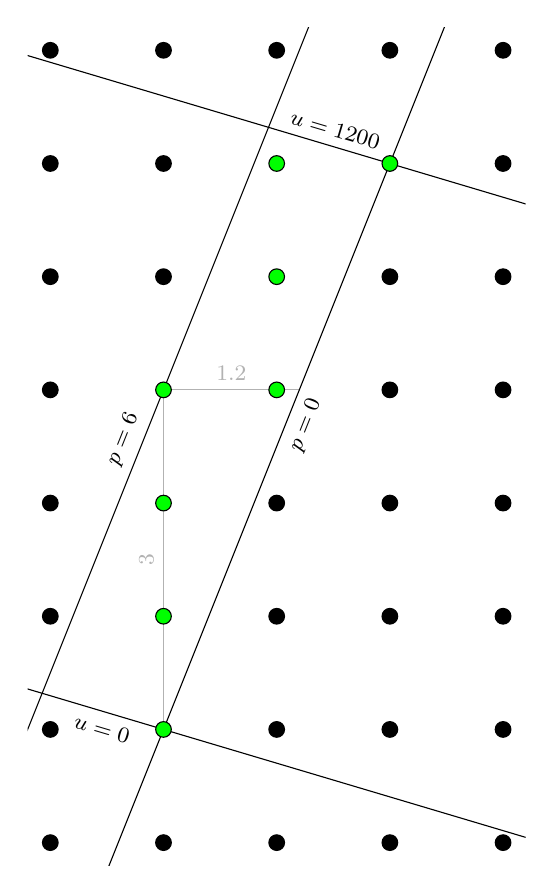
\begin{tikzpicture}[scale=1.4375]

\clip (-1 - 0.2, -1 - 0.2) rectangle (3 + 0.2, 6 + 0.2);

\draw[gray!60] (0, 0) -- (0, 1.5) node[above, rotate=90] {\footnotesize $3$} -- (0, 3);
\draw[gray!60] (0, 3) -- (0.6, 3) node[above] {\footnotesize $1.2$} -- (1.2, 3);

\draw (0 - 2, 0 - 5) -- (0 + 0.55 * 2, 0 + 0.55 * 5) node[below, rotate=68.2] {\footnotesize $p=0$} -- (0 + 2 * 2, 0 + 2 * 5);
\draw (0 - 2, 3 - 5) -- (0 - 0.1 * 2, 3 - 0.1 * 5) node[above, rotate=68.2] {\footnotesize $p=6$} -- (0 + 2 * 2, 3 + 2 * 5);

\draw (-2, -2 * -63.90/214.44) -- (-0.5, -0.5 * -63.90/214.44) node[below, rotate=-16.59] {\footnotesize $u=0$} -- (7, 7 * -63.90/214.44);
\draw
    (-2, -2 * -63.90/214.44 + 1200/214.44) --
    (1.475, 1.475 * -63.90/214.44 + 1200/214.44) node[above, rotate=-16.59] {\footnotesize $u=1200$} --
    (7, 7 * -63.90/214.44 + 1200/214.44);
\draw (-1, -1) node[circle,draw=black,fill=black,inner sep=2pt] {};
\draw (-1, 0) node[circle,draw=black,fill=black,inner sep=2pt] {};
\draw (-1, 1) node[circle,draw=black,fill=black,inner sep=2pt] {};
\draw (-1, 2) node[circle,draw=black,fill=black,inner sep=2pt] {};
\draw (-1, 3) node[circle,draw=black,fill=black,inner sep=2pt] {};
\draw (-1, 4) node[circle,draw=black,fill=black,inner sep=2pt] {};
\draw (-1, 5) node[circle,draw=black,fill=black,inner sep=2pt] {};
\draw (-1, 6) node[circle,draw=black,fill=black,inner sep=2pt] {};
\draw (0, -1) node[circle,draw=black,fill=black,inner sep=2pt] {};
\draw (0, 0) node[circle,draw=black,fill=green,inner sep=2pt] {};
\draw (0, 1) node[circle,draw=black,fill=green,inner sep=2pt] {};
\draw (0, 2) node[circle,draw=black,fill=green,inner sep=2pt] {};
\draw (0, 3) node[circle,draw=black,fill=green,inner sep=2pt] {};
\draw (0, 4) node[circle,draw=black,fill=black,inner sep=2pt] {};
\draw (0, 5) node[circle,draw=black,fill=black,inner sep=2pt] {};
\draw (0, 6) node[circle,draw=black,fill=black,inner sep=2pt] {};
\draw (1, -1) node[circle,draw=black,fill=black,inner sep=2pt] {};
\draw (1, 0) node[circle,draw=black,fill=black,inner sep=2pt] {};
\draw (1, 1) node[circle,draw=black,fill=black,inner sep=2pt] {};
\draw (1, 2) node[circle,draw=black,fill=black,inner sep=2pt] {};
\draw (1, 3) node[circle,draw=black,fill=green,inner sep=2pt] {};
\draw (1, 4) node[circle,draw=black,fill=green,inner sep=2pt] {};
\draw (1, 5) node[circle,draw=black,fill=green,inner sep=2pt] {};
\draw (1, 6) node[circle,draw=black,fill=black,inner sep=2pt] {};
\draw (2, -1) node[circle,draw=black,fill=black,inner sep=2pt] {};
\draw (2, 0) node[circle,draw=black,fill=black,inner sep=2pt] {};
\draw (2, 1) node[circle,draw=black,fill=black,inner sep=2pt] {};
\draw (2, 2) node[circle,draw=black,fill=black,inner sep=2pt] {};
\draw (2, 3) node[circle,draw=black,fill=black,inner sep=2pt] {};
\draw (2, 4) node[circle,draw=black,fill=black,inner sep=2pt] {};
\draw (2, 5) node[circle,draw=black,fill=green,inner sep=2pt] {};
\draw (2, 6) node[circle,draw=black,fill=black,inner sep=2pt] {};
\draw (3, -1) node[circle,draw=black,fill=black,inner sep=2pt] {};
\draw (3, 0) node[circle,draw=black,fill=black,inner sep=2pt] {};
\draw (3, 1) node[circle,draw=black,fill=black,inner sep=2pt] {};
\draw (3, 2) node[circle,draw=black,fill=black,inner sep=2pt] {};
\draw (3, 3) node[circle,draw=black,fill=black,inner sep=2pt] {};
\draw (3, 4) node[circle,draw=black,fill=black,inner sep=2pt] {};
\draw (3, 5) node[circle,draw=black,fill=black,inner sep=2pt] {};
\draw (3, 6) node[circle,draw=black,fill=black,inner sep=2pt] {};
\end{tikzpicture}

\vspace{1.35cm}
\caption{}
\label{fig:lattice-parallelogram}
\end{subfigure}
\caption{Lattice showing the parallelogram defining a moment of symmetry.}
\label{fig:lattice}
\end{figure}

So once we have a basis which gives increasing pitch along rows and up columns,
there's a reasonably intuitive construction for scales made up of two step
sizes, and in particular moments of symmetry. The Gral method's job here is to
provide such bases.

One last bit of MOS keyboard geometry will prove useful later. It turns out
that for an $m/n$ MOS with generator $g$ cents and period $h$ cents, on the
$m/n$ keyboard the position of the generator $(a, b)$ is related to the
position of the period $(c, d)$ by
\begin{align}
    a   &=  \left\lfloor \frac{g}{h} c \right\rfloor    \label{eq:floor} \\
    b   &=  \left\lceil  \frac{g}{h} d \right\rceil,    \label{eq:ceil}
\end{align}
where $\lfloor x \rfloor$ is the floor function (largest integer $\leq x$) and
$\lceil x \rceil$ is the ceiling function (smallest integer $\geq
x$).\footnote{You can show this by writing the step sizes $\sigma = -dg + bh$
and $\tau = cg - ah$ as $\sigma = (-dg)\bmod h$ and $\tau = cg \bmod h$ and
using the identities $x \bmod y = x - y \lfloor x/y \rfloor$ and $\lfloor -x
\rfloor = - \lceil x \rceil$, see \cite[Chapter~3]{knuth1994concrete}.}
Geometrically this means that we can find the position of the generator by
drawing a line from the root to the period, marking a point $g/h$ of the way
along the line, then taking the nearest lattice point on the left and above.
Figure \ref{fig:as-above-so-below} shows this construction on the 3/5 keyboard
for a generator of $g = 702$ cents, period $h = 1200$ cents, so $g/h = 0.585$.

The construction of Figure \ref{fig:as-above-so-below} also gives a geometrical
picture of the generator size ranges produced by the Gral method. The gray
square in Figure \ref{fig:as-above-so-below} shows all the points which would
be mapped to $(a, b)$ by Equations \ref{eq:floor} and \ref{eq:ceil}. Thinking
about similar triangles, you can see that the root-period line cuts this square
at points $a/c$ and $b/d$ of the way along its length, as marked on Figure
\ref{fig:as-above-so-below}; these are the smallest and largest generator sizes
that will produce an $m/n$ MOS.

\begin{figure}
\centering
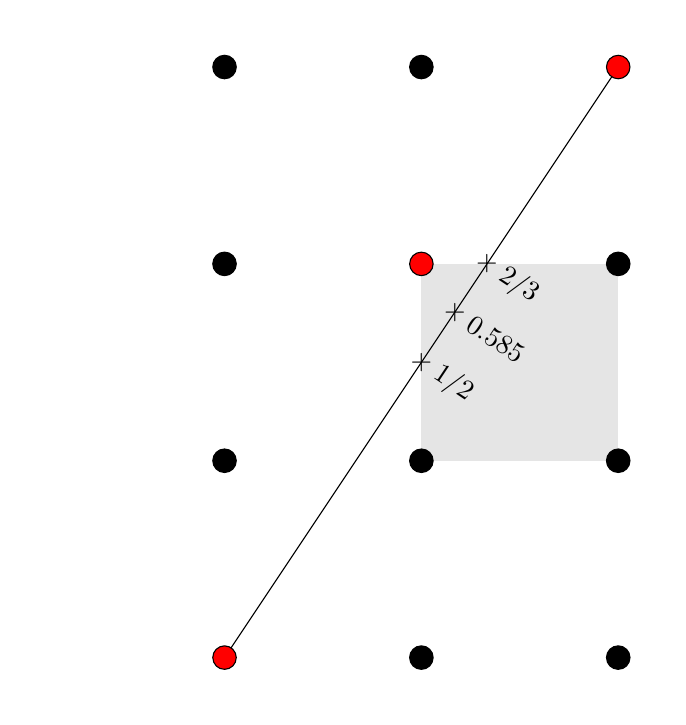
\begin{tikzpicture}[scale=2.5]

\clip (0 - 1, 0 - 0.2) rectangle (2 + 0.2, 3 + 0.2);
\fill[fill=gray!20] (1, 1) rectangle (2, 2);
\draw (0, 0) -- (0 + 2, 0 + 3);
\draw (1, 3/2) node[] {$+$};
\draw (1, 3/2) node[right, rotate=-33.690067525979785] {\;1/2};
\draw (1.17, 1.755) node[] {$+$};
\draw (1.17, 1.755) node[right, rotate=-33.690067525979785] {\;0.585};
\draw (4/3, 2) node[] {$+$};
\draw (4/3, 2) node[right, rotate=-33.690067525979785] {\;2/3};
\draw (0, 0) node[circle,draw=black,fill=red,inner sep=3pt] {};
\draw (0, 1) node[circle,draw=black,fill=black,inner sep=3pt] {};
\draw (0, 2) node[circle,draw=black,fill=black,inner sep=3pt] {};
\draw (0, 3) node[circle,draw=black,fill=black,inner sep=3pt] {};
\draw (1, 0) node[circle,draw=black,fill=black,inner sep=3pt] {};
\draw (1, 1) node[circle,draw=black,fill=black,inner sep=3pt] {};
\draw (1, 2) node[circle,draw=black,fill=red,inner sep=3pt] {};
\draw (1, 3) node[circle,draw=black,fill=black,inner sep=3pt] {};
\draw (2, 0) node[circle,draw=black,fill=black,inner sep=3pt] {};
\draw (2, 1) node[circle,draw=black,fill=black,inner sep=3pt] {};
\draw (2, 2) node[circle,draw=black,fill=black,inner sep=3pt] {};
\draw (2, 3) node[circle,draw=black,fill=red,inner sep=3pt] {};

\end{tikzpicture}

\caption{Finding the generator position from the line between root and octave
on the 3/5 keyboard.}
\label{fig:as-above-so-below}
\end{figure}

In the Gral spectrum \cite{wilsongralspectrum} Wilson shows not only the basis
for each keyboard, but also the line joining the root and octave and the notes
in the corresponding MOS. Wilson applies the Gral method to find moments of
symmetry in \cite[14-47]{wilsondiophantinetemper} and
\cite{wilsondiophantinerecur}.  Wilson also calculates MOS with his $1/x$
method together with his zig-zag patterns, for example
\cite[3]{wilsondiophantinerecur}. The equivalence of the Gral and zig-zag
methods is a purely mathematical result on continued fractions, explained very
clearly in \cite{richards1981continued}. For much more on continued fractions
and lattices see \cite{karpenkov2022geometry}. Wilson calculates some moments
of symmetry with a non-octave period, for example stacking a generator of 10/7,
$g = 617$ cents, within a period of 13/7, $h = 1072$ cents
\cite[7]{wilsonnonoctave}.

\clearpage
\section{Secondary moments of symmetry}
Secondary MOS are smaller scales derived from a larger MOS. This appendix gives
keyboard mappings which make secondary MOS easy to play. The general idea is
that you can play secondary MOS by shifting the same shape around a suitably
chosen keyboard mapping, and so let your fingers do the thinking.

\subsection{The Tanabe cycle}
Let's start with the Tanabe cycle \cite[13]{wilsonmos}, which is based on
stacking pure fourths. Table \ref{tab:gral-mos-4-3} shows the MOS we get from
stacking $4/3$ within an octave. Take the 3/7 MOS as the parent MOS, using the
mode with chain positions between $-5$ and $+1$. Now map the parent MOS by
scale degree, taking the generator (scale degree 3) and the period (scale
degree 7) to form a basis. Table \ref{tab:gral-3-7} shows the Gral method
applied to 3/7 --- choose the 2/5 keyboard. Figure \ref{fig:tanabe-mapping}
shows the 3/7 parent MOS mapped to the 2/5 keyboard.

\begin{table}
\centering
\begin{tabular}{rr@{\hspace{1cm}}r@{\hspace{1cm}}rr@{\hspace{1cm}}rr@{\hspace{1cm}}rr}
\toprule
Left    &   Right   &   Mediant &   $a$  &  $b$  &  $c$  &  $d$  &  $s$  &  $t$  \\
\midrule
$0/1$ & $1/0$ & $1/1$ & $0$ & $1$ & $1$ & $0$ & $1200.000$ & $498.045$ \\
      & $1/1$ & $1/2$ & $0$ & $1$ & $1$ & $1$ & $701.955$ & $498.045$ \\
      & $1/2$ & $1/3$ & $0$ & $1$ & $1$ & $2$ & $203.910$ & $498.045$ \\
$1/3$ &       & $2/5$ & $1$ & $1$ & $3$ & $2$ & $203.910$ & $294.135$ \\
$2/5$ &       & $3/7$ & $2$ & $1$ & $5$ & $2$ & $203.910$ & $90.225$ \\
      & $3/7$ & $5/12$ & $2$ & $3$ & $5$ & $7$ & $113.685$ & $90.225$ \\
      & $5/12$ & $7/17$ & $2$ & $5$ & $5$ & $12$ & $23.460$ & $90.225$ \\
$7/17$ &       & $12/29$ & $7$ & $5$ & $17$ & $12$ & $23.460$ & $66.765$ \\
$12/29$ &       & $17/41$ & $12$ & $5$ & $29$ & $12$ & $23.460$ & $43.305$ \\
$\vdots\quad$ & $\vdots\quad$ & $\vdots\quad$ & $\vdots\;$ & $\vdots\;$ & $\vdots\;$ & $\vdots\;$ & $\vdots\;$ & $\vdots\;$ \\
\bottomrule
\end{tabular}
\caption{Gral method for MOS with generator $g = 498.045$ cents and period $h =
1200$ cents.}
\label{tab:gral-mos-4-3}
\end{table}

\begin{table}
\vspace{3ex}
\centering
\begin{tabular}{rr@{\hspace{1cm}}r@{\hspace{1cm}}rr@{\hspace{1cm}}rr@{\hspace{1cm}}rr}
\toprule
Left    &   Right   &   Mediant &   $a$  &  $b$  &  $c$  &  $d$  &  $s$  &  $t$  \\
\midrule
$0/1$ & $1/0$ & $1/1$ & $0$ & $1$ & $1$ & $0$ & $7$ & $3$ \\
      & $1/1$ & $1/2$ & $0$ & $1$ & $1$ & $1$ & $4$ & $3$ \\
      & $1/2$ & $1/3$ & $0$ & $1$ & $1$ & $2$ & $1$ & $3$ \\
$1/3$ &       & $2/5$ & $1$ & $1$ & $3$ & $2$ & $1$ & $2$ \\
$2/5$ &       & $3/7$ & $2$ & $1$ & $5$ & $2$ & $1$ & $1$ \\
\bottomrule
\end{tabular}
\caption{Gral method applied to 3/7.}
\label{tab:gral-3-7}
\end{table}

Playing the 2/5 MOS shape, with chain positions between $-4$ and $0$, starting
at 1/1 gives the ordinary 2/5 MOS from stacking $4/3$, shown in Figure
\ref{fig:secondary-mos-keyboards-1}. Playing the same 2/5 MOS shape starting on
notes moving around the circle of fourths seven times gives a cycle of seven
secondary MOS. Figure \ref{fig:secondary-mos-keyboards} shows these shapes
starting on chain positions $-1$ through $+5$; this matches the order of the
scales in the Tanabe cycle diagram in \cite[13]{wilsonmos}.

\begin{figure}
\input{secondary-mos-tanabe-basis.tex}
\caption{Keyboard mapping for the Tanabe cycle.}
\label{fig:tanabe-mapping}
\end{figure}

\newgeometry{top=10mm, bottom=20mm, left=10mm, right=10mm}
\bgroup
\NiceMatrixOptions{cell-space-limits = 2pt}
\begin{figure}
\begin{subfigure}{0.5\textwidth}
\input{secondary-mos-tanabe-0.tex}
\vspace{-0.5cm}
\caption{}
\label{fig:secondary-mos-keyboards-0}
\vspace{0.25cm}
\end{subfigure}
\begin{subfigure}{0.5\textwidth}
\input{secondary-mos-tanabe-1.tex}
\vspace{-0.5cm}
\caption{}
\vspace{0.25cm}
\label{fig:secondary-mos-keyboards-1}
\end{subfigure}
\begin{subfigure}{0.5\textwidth}
\input{secondary-mos-tanabe-2.tex}
\vspace{-0.5cm}
\caption{}
\vspace{0.25cm}
\end{subfigure}
\begin{subfigure}{0.5\textwidth}
\begin{center}
$\begin{NiceArray}[small, first-col, last-row, columns-width=1.1cm]{|c|c|c|c|c|c|c|}
\hline
 &    \scriptstyle \scriptstyle \raisebox{.2\height}{\scalebox{.6}{+}}14\ \ \ 7.
 &    \scriptstyle \scriptstyle \raisebox{.2\height}{\scalebox{.6}{+}}12\ \ \ 8.
 &    \scriptstyle \scriptstyle \raisebox{.2\height}{\scalebox{.6}{+}}10\ \ \ 9.
 &    \scriptstyle \scriptstyle \raisebox{.2\height}{\scalebox{.6}{+}}8\ \ \ 10.
 &    \scriptstyle \scriptstyle \raisebox{.2\height}{\scalebox{.6}{+}}6\ \ \ 11.
 &    \scriptstyle \scriptstyle \raisebox{.2\height}{\scalebox{.6}{+}}4\ \ \ 12.
 &\cellcolor{green!25}     \scriptstyle \scriptstyle \raisebox{.2\height}{\scalebox{.6}{+}}2\ \ \ 13.
\\
4 &    2/1
 &    9/4
 &    81/32
 &    8/3
 &    3/1
 &    27/8
 &\cellcolor{green!25}     243/64
\\
 &    \scriptstyle 1200
 &    \scriptstyle 1404
 &    \scriptstyle 1608
 &    \scriptstyle 1698
 &    \scriptstyle 1902
 &    \scriptstyle 2106
 &\cellcolor{green!25}     \scriptstyle 2310
\\
\hline
 &    \scriptstyle \scriptstyle \raisebox{.2\height}{\scalebox{.6}{+}}11\ \ \ 5.
 &    \scriptstyle \scriptstyle \raisebox{.2\height}{\scalebox{.6}{+}}9\ \ \ 6.
 &    \scriptstyle \scriptstyle \raisebox{.2\height}{\scalebox{.6}{+}}7\ \ \ 7.
 &    \scriptstyle \scriptstyle \raisebox{.2\height}{\scalebox{.6}{+}}5\ \ \ 8.
 &    \scriptstyle \scriptstyle \raisebox{.2\height}{\scalebox{.6}{+}}3\ \ \ 9.
 &\cellcolor{green!25}     \scriptstyle \scriptstyle \raisebox{.2\height}{\scalebox{.6}{+}}1\ \ \ 10.
 &\cellcolor{green!25}     \scriptstyle \scriptstyle \raisebox{.2\height}{\scalebox{.8}{-}}1\ \ \ 11.
\\
3 &    27/16
 &    243/128
 &    2/1
 &    9/4
 &    81/32
 &\cellcolor{green!25}     8/3
 &\cellcolor{green!25}     3/1
\\
 &    \scriptstyle 906
 &    \scriptstyle 1110
 &    \scriptstyle 1200
 &    \scriptstyle 1404
 &    \scriptstyle 1608
 &\cellcolor{green!25}     \scriptstyle 1698
 &\cellcolor{green!25}     \scriptstyle 1902
\\
\hline
 &    \scriptstyle \scriptstyle \raisebox{.2\height}{\scalebox{.6}{+}}8\ \ \ 3.
 &    \scriptstyle \scriptstyle \raisebox{.2\height}{\scalebox{.6}{+}}6\ \ \ 4.
 &    \scriptstyle \scriptstyle \raisebox{.2\height}{\scalebox{.6}{+}}4\ \ \ 5.
 &\cellcolor{green!25}     \scriptstyle \scriptstyle \raisebox{.2\height}{\scalebox{.6}{+}}2\ \ \ 6.
 &\cellcolor{green!25}     \scriptstyle \scriptstyle \raisebox{.2\height}{\scalebox{.6}{+}}0\ \ \ 7.
 &\cellcolor{green!25}     \scriptstyle \scriptstyle \raisebox{.2\height}{\scalebox{.8}{-}}2\ \ \ 8.
 &    \scriptstyle \scriptstyle \raisebox{.2\height}{\scalebox{.8}{-}}4\ \ \ 9.
\\
2 &    4/3
 &    3/2
 &    27/16
 &\cellcolor{green!25}     243/128
 &\cellcolor{green!25}     2/1
 &\cellcolor{green!25}     9/4
 &    81/32
\\
 &    \scriptstyle 498
 &    \scriptstyle 702
 &    \scriptstyle 906
 &\cellcolor{green!25}     \scriptstyle 1110
 &\cellcolor{green!25}     \scriptstyle 1200
 &\cellcolor{green!25}     \scriptstyle 1404
 &    \scriptstyle 1608
\\
\hline
 &    \scriptstyle \scriptstyle \raisebox{.2\height}{\scalebox{.6}{+}}5\ \ \ 1.
 &    \scriptstyle \scriptstyle \raisebox{.2\height}{\scalebox{.6}{+}}3\ \ \ 2.
 &    \scriptstyle \scriptstyle \raisebox{.2\height}{\scalebox{.6}{+}}1\ \ \ 3.
 &    \scriptstyle \scriptstyle \raisebox{.2\height}{\scalebox{.8}{-}}1\ \ \ 4.
 &    \scriptstyle \scriptstyle \raisebox{.2\height}{\scalebox{.8}{-}}3\ \ \ 5.
 &    \scriptstyle \scriptstyle \raisebox{.2\height}{\scalebox{.8}{-}}5\ \ \ 6.
 &    \scriptstyle \scriptstyle \raisebox{.2\height}{\scalebox{.8}{-}}7\ \ \ 7.
\\
1 &    9/8
 &    81/64
 &    4/3
 &    3/2
 &    27/16
 &    243/128
 &    2/1
\\
 &    \scriptstyle 204
 &    \scriptstyle 408
 &    \scriptstyle 498
 &    \scriptstyle 702
 &    \scriptstyle 906
 &    \scriptstyle 1110
 &    \scriptstyle 1200
\\
\hline
 &    \scriptstyle \scriptstyle \raisebox{.2\height}{\scalebox{.6}{+}}2\ \ \ \raisebox{.2\height}{\scalebox{.8}{-}}1.
 &    \scriptstyle \scriptstyle \raisebox{.2\height}{\scalebox{.6}{+}}0\ \ \ 0.
 &    \scriptstyle \scriptstyle \raisebox{.2\height}{\scalebox{.8}{-}}2\ \ \ 1.
 &    \scriptstyle \scriptstyle \raisebox{.2\height}{\scalebox{.8}{-}}4\ \ \ 2.
 &    \scriptstyle \scriptstyle \raisebox{.2\height}{\scalebox{.8}{-}}6\ \ \ 3.
 &    \scriptstyle \scriptstyle \raisebox{.2\height}{\scalebox{.8}{-}}8\ \ \ 4.
 &    \scriptstyle \scriptstyle \raisebox{.2\height}{\scalebox{.8}{-}}10\ \ \ 5.
\\
0 &    243/256
 &    1/1
 &    9/8
 &    81/64
 &    4/3
 &    3/2
 &    27/16
\\
 &    \scriptstyle -90
 &    \scriptstyle 0
 &    \scriptstyle 204
 &    \scriptstyle 408
 &    \scriptstyle 498
 &    \scriptstyle 702
 &    \scriptstyle 906
\\
\hline
& -1 & 0 & 1 & 2 & 3 & 4 & 5
\end{NiceArray}$
\end{center}

\vspace{-0.5cm}
\caption{}
\vspace{0.25cm}
\end{subfigure}
\begin{subfigure}{0.5\textwidth}
\input{secondary-mos-tanabe-4.tex}
\vspace{-0.5cm}
\caption{}
\vspace{0.25cm}
\end{subfigure}
\begin{subfigure}{0.5\textwidth}
\input{secondary-mos-tanabe-5.tex}
\vspace{-0.5cm}
\caption{}
\vspace{0.25cm}
\end{subfigure}
\begin{subfigure}{0.5\textwidth}
\input{secondary-mos-tanabe-6.tex}
\vspace{-0.5cm}
\caption{}
\vspace{0.25cm}
\end{subfigure}
\caption{Secondary MOS from the Tanabe cycle.}
\label{fig:secondary-mos-keyboards}
\end{figure}
\egroup

\restoregeometry

Figure \ref{fig:secondary-mos-steps} shows the scale tones and scale steps for
the scales in Figure \ref{fig:secondary-mos-keyboards}. The first row gives the
scale in Figure \ref{fig:secondary-mos-keyboards-0}, the second in
\ref{fig:secondary-mos-keyboards-1}, and so on. There are four step sizes
involved, the two steps sizes $9/8$ and $32/27$ from the ordinary 2/5 MOS, and
two new step sizes $256/243$ and $81/64$. Looking at the keyboard diagrams, the
steps $9/8$ and $256/243$ come from moving along a row, and the steps $32/27$
and $81/64$ come from moving up a column.

\begin{figure}
\bgroup
\def\arraystretch{2}
\begin{center}
\begin{tabular}{rrrrrrrrrrr}
\small $\mathcolor{gray}{\frac{3}{2}}$ & \Large $\frac{9}{8}$ & \small $\mathcolor{gray}{\frac{27}{16}}$ & \Large $\frac{9}{8}$ & \small $\mathcolor{gray}{\frac{243}{128}}$ & \Large $\frac{32}{27}$ & \small $\mathcolor{gray}{\frac{9}{4}}$ & \Large $\frac{9}{8}$ & \small $\mathcolor{gray}{\frac{81}{32}}$ & \Large $\frac{32}{27}$ & \small $\mathcolor{gray}{\frac{3}{1}}$ \\
\small $\mathcolor{gray}{\frac{1}{1}}$ & \Large $\frac{9}{8}$ & \small $\mathcolor{gray}{\frac{9}{8}}$ & \Large $\frac{9}{8}$ & \small $\mathcolor{gray}{\frac{81}{64}}$ & \Large $\frac{32}{27}$ & \small $\mathcolor{gray}{\frac{3}{2}}$ & \Large $\frac{9}{8}$ & \small $\mathcolor{gray}{\frac{27}{16}}$ & \Large $\frac{32}{27}$ & \small $\mathcolor{gray}{\frac{2}{1}}$ \\
\small $\mathcolor{gray}{\frac{4}{3}}$ & \Large $\frac{9}{8}$ & \small $\mathcolor{gray}{\frac{3}{2}}$ & \Large $\frac{9}{8}$ & \small $\mathcolor{gray}{\frac{27}{16}}$ & \Large $\frac{32}{27}$ & \small $\mathcolor{gray}{\frac{2}{1}}$ & \Large $\frac{9}{8}$ & \small $\mathcolor{gray}{\frac{9}{4}}$ & \Large $\frac{32}{27}$ & \small $\mathcolor{gray}{\frac{8}{3}}$ \\
\small $\mathcolor{gray}{\frac{243}{128}}$ & \Large $\frac{256}{243}$ & \small $\mathcolor{gray}{\frac{2}{1}}$ & \Large $\frac{9}{8}$ & \small $\mathcolor{gray}{\frac{9}{4}}$ & \Large $\frac{32}{27}$ & \small $\mathcolor{gray}{\frac{8}{3}}$ & \Large $\frac{9}{8}$ & \small $\mathcolor{gray}{\frac{3}{1}}$ & \Large $\frac{81}{64}$ & \small $\mathcolor{gray}{\frac{243}{64}}$ \\
\small $\mathcolor{gray}{\frac{81}{64}}$ & \Large $\frac{256}{243}$ & \small $\mathcolor{gray}{\frac{4}{3}}$ & \Large $\frac{9}{8}$ & \small $\mathcolor{gray}{\frac{3}{2}}$ & \Large $\frac{81}{64}$ & \small $\mathcolor{gray}{\frac{243}{128}}$ & \Large $\frac{256}{243}$ & \small $\mathcolor{gray}{\frac{2}{1}}$ & \Large $\frac{81}{64}$ & \small $\mathcolor{gray}{\frac{81}{32}}$ \\
\small $\mathcolor{gray}{\frac{27}{16}}$ & \Large $\frac{9}{8}$ & \small $\mathcolor{gray}{\frac{243}{128}}$ & \Large $\frac{256}{243}$ & \small $\mathcolor{gray}{\frac{2}{1}}$ & \Large $\frac{81}{64}$ & \small $\mathcolor{gray}{\frac{81}{32}}$ & \Large $\frac{256}{243}$ & \small $\mathcolor{gray}{\frac{8}{3}}$ & \Large $\frac{81}{64}$ & \small $\mathcolor{gray}{\frac{27}{8}}$ \\
\small $\mathcolor{gray}{\frac{9}{8}}$ & \Large $\frac{9}{8}$ & \small $\mathcolor{gray}{\frac{81}{64}}$ & \Large $\frac{256}{243}$ & \small $\mathcolor{gray}{\frac{4}{3}}$ & \Large $\frac{81}{64}$ & \small $\mathcolor{gray}{\frac{27}{16}}$ & \Large $\frac{9}{8}$ & \small $\mathcolor{gray}{\frac{243}{128}}$ & \Large $\frac{32}{27}$ & \small $\mathcolor{gray}{\frac{9}{4}}$ \\
\end{tabular}

\end{center}
\egroup
\caption{Scale tones (small) and step sizes (large) for secondary MOS from
Figure \ref{fig:secondary-mos-keyboards}.\vspace{0.25cm}}
\label{fig:secondary-mos-steps}
\end{figure}

\begin{figure}
\bgroup
\NiceMatrixOptions{cell-space-limits = 5pt}
$\begin{NiceArray}[small]{rp{10pt}p{10pt}p{10pt}p{10pt}p{10pt}p{15pt}p{10pt}p{10pt}p{10pt}p{10pt}p{10pt}p{15pt}p{10pt}p{10pt}p{10pt}p{10pt}p{10pt}p{15pt}p{10pt}p{10pt}p{10pt}p{10pt}p{10pt}p{15pt}p{10pt}p{10pt}p{10pt}p{10pt}p{10pt}}
& \Block{1-29}{\mathrm{\mathbf{Mode}}} \vspace{15pt} \\
\Block{5-1}{\mathrm{\mathbf{Family}}\quad}  & $\mathrm{C}$ & $\mathrm{D}$ & $\mathrm{E}$ & $\mathrm{G}$ & $\mathrm{A}$ & & $\mathrm{C}$ & $\mathrm{D}$ & $\mathrm{F}$ & $\mathrm{G}$ & $\mathrm{B\flat}$ & & $\mathrm{C}$ & $\mathrm{E\flat}$ & $\mathrm{F}$ & $\mathrm{A\flat}$ & $\mathrm{B\flat}$ & & $\mathrm{C}$ & $\mathrm{D}$ & $\mathrm{F}$ & $\mathrm{G}$ & $\mathrm{A}$ & & $\mathrm{C}$ & $\mathrm{E\flat}$ & $\mathrm{F}$ & $\mathrm{G}$ & $\mathrm{B\flat}$ \\
& $\mathrm{C}$ & $\mathrm{D}$ & $\mathrm{F}$ & $\mathrm{G}$ & $\mathrm{B}$ & & $\mathrm{C}$ & $\mathrm{E\flat}$ & $\mathrm{F}$ & $\mathrm{A}$ & $\mathrm{B\flat}$ & & $\mathrm{C}$ & $\mathrm{D}$ & $\mathrm{F}\sharp$ & $\mathrm{G}$ & $\mathrm{A}$ & & $\mathrm{C}$ & $\mathrm{E}$ & $\mathrm{F}$ & $\mathrm{G}$ & $\mathrm{B\flat}$ & & $\mathrm{C}$ & $\mathrm{D\flat}$ & $\mathrm{E\flat}$ & $\mathrm{G\flat}$ & $\mathrm{A\flat}$ \\
& $\mathrm{C}$ & $\mathrm{E}$ & $\mathrm{F}$ & $\mathrm{G}$ & $\mathrm{B}$ & & $\mathrm{C}$ & $\mathrm{D\flat}$ & $\mathrm{E\flat}$ & $\mathrm{G}$ & $\mathrm{A\flat}$ & & $\mathrm{C}$ & $\mathrm{D}$ & $\mathrm{F}\sharp$ & $\mathrm{G}$ & $\mathrm{B}$ & & $\mathrm{C}$ & $\mathrm{E}$ & $\mathrm{F}$ & $\mathrm{A}$ & $\mathrm{B\flat}$ & & $\mathrm{C}$ & $\mathrm{D\flat}$ & $\mathrm{F}$ & $\mathrm{G\flat}$ & $\mathrm{A\flat}$ \\
& $\mathrm{C}$ & $\mathrm{E}$ & $\mathrm{F}$ & $\mathrm{A}$ & $\mathrm{B}$ & & $\mathrm{C}$ & $\mathrm{D\flat}$ & $\mathrm{F}$ & $\mathrm{G}$ & $\mathrm{A\flat}$ & & $\mathrm{C}$ & $\mathrm{E}$ & $\mathrm{F}\sharp$ & $\mathrm{G}$ & $\mathrm{B}$ & & $\mathrm{C}$ & $\mathrm{D}$ & $\mathrm{E\flat}$ & $\mathrm{G}$ & $\mathrm{A\flat}$ & & $\mathrm{C}$ & $\mathrm{D\flat}$ & $\mathrm{F}$ & $\mathrm{G\flat}$ & $\mathrm{B\flat}$ \\
& $\mathrm{C}$ & $\mathrm{E}$ & $\mathrm{F}\sharp$ & $\mathrm{A}$ & $\mathrm{B}$ & & $\mathrm{C}$ & $\mathrm{D}$ & $\mathrm{F}$ & $\mathrm{G}$ & $\mathrm{A\flat}$ & & $\mathrm{C}$ & $\mathrm{E\flat}$ & $\mathrm{F}$ & $\mathrm{G\flat}$ & $\mathrm{B\flat}$ & & $\mathrm{C}$ & $\mathrm{D}$ & $\mathrm{E\flat}$ & $\mathrm{G}$ & $\mathrm{A}$ & & $\mathrm{C}$ & $\mathrm{D\flat}$ & $\mathrm{F}$ & $\mathrm{G}$ & $\mathrm{B\flat}$ \\
\end{NiceArray}$
\egroup
\caption{The five modes of each of the five families from the Tanabe cycle.}
\label{fig:modes-tanabe}
\end{figure}

The Tanabe cycle contains seven scales but only five are unique in the sense
that they aren't modes of each other. Figure \ref{fig:modes-tanabe} shows the
modes of each of these five scales, all transposed to start on the same note
$\mathrm{C}$, where the note names give the position in the chain of $4/3$
fourths.  This gives 25 scales, the five modes of each of five families, using
thirteen pitches $\mathrm{F}\sharp$ through $\mathrm{G}\flat$ in the circle of
fourths.  These 25 scales, organized differently, are shown in Wilson's
\textit{Parallelogram from the Tanabe Cycle} \cite[14]{wilsonmos}.

\clearpage
\subsection{General secondary MOS}
When mapping a parent MOS by scale degree, we can pick a note other than the
generator of the MOS to form a basis with the period on the keyboard. Wilson
gives a cycle of 17 scales \cite[6-8]{wilsonmos} which illustrates this.  Take
the 7/17 MOS from stacking fourths (see Table \ref{tab:gral-mos-4-3}) as the
parent MOS, using the mode with chain positions between $-4$ and $+12$. Now map
this 7/17 parent MOS by scale degree, taking scale degree 5 and scale degree 17
(the period) to form a basis. Table \ref{tab:gral-5-17} shows the Gral method
applied to 5/17 --- choose the 2/7 keyboard. Figure
\ref{fig:secondary-mos-17-basis} shows the 7/17 parent MOS mapped to the 2/7
keyboard.

Playing the 2/7 MOS shape, with chain positions $0$ to $+6$, starting at notes
with chain positions $0$ through $+16$, we get a cycle of 17 scales.  Figure
\ref{fig:secondary-mos-17} shows seven of the scales in this cycle, starting at
notes with chain positions $+2$ through $+8$.

Figure \ref{fig:secondary-mos-17-steps} shows the scale tones and scale steps
for the scales in Figure \ref{fig:secondary-mos-17}. We get four step sizes,
$9/8$ or 204 cents, $2187/2048$ or 114 cents, $65536/59049$ or 180 cents, and
$16777216/14348907$ or 271 cents. The 180 cent and 114 cent steps come from
moving along a row, the 204 cent and 271 cent steps from moving up a column.

The cycle of 17 scales contains seven unique scales (which aren't modes of each
other); Figure \ref{fig:secondary-mos-17} shows just these seven scales in the
cycle. Figure \ref{fig:secondary-mos-17-modes} shows the seven modes of each of
these seven scales; the octave of 1200 cents in each scale is omitted to save
space. The scales are arranged so that when moving one row down the table, only
one note changes in the first mode. The first four families give the major,
`harmonic major', harmonic minor, and natural minor scales.  The next three
families are very close to those found in Wilson's Purvi modulations
\cite{wilson1987purvi} Figure 2b, based on the tetrachord $16/15$ $75/64$
$16/15$. These scales are also found in Wilson's Marwa permutations
\cite{wilson1986marwa} Figure 12 based on the same tetrachord.

\begin{table}
\centering
\begin{tabular}{rr@{\hspace{1cm}}r@{\hspace{1cm}}rr@{\hspace{1cm}}rr@{\hspace{1cm}}rr}
\toprule
Left    &   Right   &   Mediant &   $a$  &  $b$  &  $c$  &  $d$  &  $s$  &  $t$  \\
\midrule
$0/1$ & $1/0$ & $1/1$ & $0$ & $1$ & $1$ & $0$ & $17$ & $5$ \\
      & $1/1$ & $1/2$ & $0$ & $1$ & $1$ & $1$ & $12$ & $5$ \\
      & $1/2$ & $1/3$ & $0$ & $1$ & $1$ & $2$ & $7$ & $5$ \\
      & $1/3$ & $1/4$ & $0$ & $1$ & $1$ & $3$ & $2$ & $5$ \\
$1/4$ &       & $2/7$ & $1$ & $1$ & $4$ & $3$ & $2$ & $3$ \\
$2/7$ &       & $3/10$ & $2$ & $1$ & $7$ & $3$ & $2$ & $1$ \\
      & $3/10$ & $5/17$ & $2$ & $3$ & $7$ & $10$ & $1$ & $1$ \\
\bottomrule
\end{tabular}
\caption{Gral method applied to 5/17.}
\label{tab:gral-5-17}
\end{table}

\begin{figure}
\input{secondary-mos-17-basis.tex}
\caption{Keyboard mapping for Wilson's cycle of 17 scales.}
\label{fig:secondary-mos-17-basis}
\end{figure}

\newgeometry{top=5mm, bottom=20mm, left=10mm, right=10mm}
\bgroup
\NiceMatrixOptions{cell-space-limits = 2pt}
\begin{figure}
\begin{subfigure}{\textwidth}
\input{secondary-mos-17-0.tex}
\vspace{0.0cm}
\end{subfigure}
\begin{subfigure}{\textwidth}
\begin{center}
$\begin{NiceArray}[small, first-col, last-row, columns-width=1.1cm]{|c|c|c|c|c|c|c|c|c|}
\hline
 &    \scriptstyle \scriptstyle \raisebox{.2\height}{\scalebox{.6}{+}}27\ \ \ 16.
 &    \scriptstyle \scriptstyle \raisebox{.2\height}{\scalebox{.6}{+}}24\ \ \ 18.
 &    \scriptstyle \scriptstyle \raisebox{.2\height}{\scalebox{.6}{+}}21\ \ \ 20.
 &    \scriptstyle \scriptstyle \raisebox{.2\height}{\scalebox{.6}{+}}18\ \ \ 22.
 &    \scriptstyle \scriptstyle \raisebox{.2\height}{\scalebox{.6}{+}}15\ \ \ 24.
 &    \scriptstyle \scriptstyle \raisebox{.2\height}{\scalebox{.6}{+}}12\ \ \ 26.
 &\cellcolor{green!25}     \scriptstyle \scriptstyle \raisebox{.2\height}{\scalebox{.6}{+}}9\ \ \ 28.
 &\cellcolor{green!25}     \scriptstyle \scriptstyle \raisebox{.2\height}{\scalebox{.6}{+}}6\ \ \ 30.
 &\cellcolor{green!25}     \scriptstyle \scriptstyle \raisebox{.2\height}{\scalebox{.6}{+}}3\ \ \ 32.
\\
6 &    G^{12}
 &    G^{5}
 &    G^{-2}
 &    G^{8}
 &    G^{1}
 &    G^{11}
 &\cellcolor{green!25}     G^{4}
 &\cellcolor{green!25}     G^{-3}
 &\cellcolor{green!25}     G^{7}
\\
 &    \scriptstyle 1177
 &    \scriptstyle 1290
 &    \scriptstyle 1404
 &    \scriptstyle 1584
 &    \scriptstyle 1698
 &    \scriptstyle 1878
 &\cellcolor{green!25}     \scriptstyle 1992
 &\cellcolor{green!25}     \scriptstyle 2106
 &\cellcolor{green!25}     \scriptstyle 2286
\\
\hline
 &    \scriptstyle \scriptstyle \raisebox{.2\height}{\scalebox{.6}{+}}23\ \ \ 13.
 &    \scriptstyle \scriptstyle \raisebox{.2\height}{\scalebox{.6}{+}}20\ \ \ 15.
 &    \scriptstyle \scriptstyle \raisebox{.2\height}{\scalebox{.6}{+}}17\ \ \ 17.
 &    \scriptstyle \scriptstyle \raisebox{.2\height}{\scalebox{.6}{+}}14\ \ \ 19.
 &    \scriptstyle \scriptstyle \raisebox{.2\height}{\scalebox{.6}{+}}11\ \ \ 21.
 &\cellcolor{green!25}     \scriptstyle \scriptstyle \raisebox{.2\height}{\scalebox{.6}{+}}8\ \ \ 23.
 &\cellcolor{green!25}     \scriptstyle \scriptstyle \raisebox{.2\height}{\scalebox{.6}{+}}5\ \ \ 25.
 &    \scriptstyle \scriptstyle \raisebox{.2\height}{\scalebox{.6}{+}}2\ \ \ 27.
 &    \scriptstyle \scriptstyle \raisebox{.2\height}{\scalebox{.8}{-}}1\ \ \ 29.
\\
5 &    G^{-3}
 &    G^{7}
 &    G^{0}
 &    G^{10}
 &    G^{3}
 &\cellcolor{green!25}     G^{-4}
 &\cellcolor{green!25}     G^{6}
 &    G^{-1}
 &    G^{9}
\\
 &    \scriptstyle 906
 &    \scriptstyle 1086
 &    \scriptstyle 1200
 &    \scriptstyle 1380
 &    \scriptstyle 1494
 &\cellcolor{green!25}     \scriptstyle 1608
 &\cellcolor{green!25}     \scriptstyle 1788
 &    \scriptstyle 1902
 &    \scriptstyle 2082
\\
\hline
 &    \scriptstyle \scriptstyle \raisebox{.2\height}{\scalebox{.6}{+}}19\ \ \ 10.
 &    \scriptstyle \scriptstyle \raisebox{.2\height}{\scalebox{.6}{+}}16\ \ \ 12.
 &    \scriptstyle \scriptstyle \raisebox{.2\height}{\scalebox{.6}{+}}13\ \ \ 14.
 &    \scriptstyle \scriptstyle \raisebox{.2\height}{\scalebox{.6}{+}}10\ \ \ 16.
 &\cellcolor{green!25}     \scriptstyle \scriptstyle \raisebox{.2\height}{\scalebox{.6}{+}}7\ \ \ 18.
 &\cellcolor{green!25}     \scriptstyle \scriptstyle \raisebox{.2\height}{\scalebox{.6}{+}}4\ \ \ 20.
 &    \scriptstyle \scriptstyle \raisebox{.2\height}{\scalebox{.6}{+}}1\ \ \ 22.
 &    \scriptstyle \scriptstyle \raisebox{.2\height}{\scalebox{.8}{-}}2\ \ \ 24.
 &    \scriptstyle \scriptstyle \raisebox{.2\height}{\scalebox{.8}{-}}5\ \ \ 26.
\\
4 &    G^{-1}
 &    G^{9}
 &    G^{2}
 &    G^{12}
 &\cellcolor{green!25}     G^{5}
 &\cellcolor{green!25}     G^{-2}
 &    G^{8}
 &    G^{1}
 &    G^{11}
\\
 &    \scriptstyle 702
 &    \scriptstyle 882
 &    \scriptstyle 996
 &    \scriptstyle 1177
 &\cellcolor{green!25}     \scriptstyle 1290
 &\cellcolor{green!25}     \scriptstyle 1404
 &    \scriptstyle 1584
 &    \scriptstyle 1698
 &    \scriptstyle 1878
\\
\hline
 &    \scriptstyle \scriptstyle \raisebox{.2\height}{\scalebox{.6}{+}}15\ \ \ 7.
 &    \scriptstyle \scriptstyle \raisebox{.2\height}{\scalebox{.6}{+}}12\ \ \ 9.
 &    \scriptstyle \scriptstyle \raisebox{.2\height}{\scalebox{.6}{+}}9\ \ \ 11.
 &    \scriptstyle \scriptstyle \raisebox{.2\height}{\scalebox{.6}{+}}6\ \ \ 13.
 &\cellcolor{green!25}     \scriptstyle \scriptstyle \raisebox{.2\height}{\scalebox{.6}{+}}3\ \ \ 15.
 &    \scriptstyle \scriptstyle \raisebox{.2\height}{\scalebox{.6}{+}}0\ \ \ 17.
 &    \scriptstyle \scriptstyle \raisebox{.2\height}{\scalebox{.8}{-}}3\ \ \ 19.
 &    \scriptstyle \scriptstyle \raisebox{.2\height}{\scalebox{.8}{-}}6\ \ \ 21.
 &    \scriptstyle \scriptstyle \raisebox{.2\height}{\scalebox{.8}{-}}9\ \ \ 23.
\\
3 &    G^{1}
 &    G^{11}
 &    G^{4}
 &    G^{-3}
 &\cellcolor{green!25}     G^{7}
 &    G^{0}
 &    G^{10}
 &    G^{3}
 &    G^{-4}
\\
 &    \scriptstyle 498
 &    \scriptstyle 678
 &    \scriptstyle 792
 &    \scriptstyle 906
 &\cellcolor{green!25}     \scriptstyle 1086
 &    \scriptstyle 1200
 &    \scriptstyle 1380
 &    \scriptstyle 1494
 &    \scriptstyle 1608
\\
\hline
 &    \scriptstyle \scriptstyle \raisebox{.2\height}{\scalebox{.6}{+}}11\ \ \ 4.
 &    \scriptstyle \scriptstyle \raisebox{.2\height}{\scalebox{.6}{+}}8\ \ \ 6.
 &    \scriptstyle \scriptstyle \raisebox{.2\height}{\scalebox{.6}{+}}5\ \ \ 8.
 &    \scriptstyle \scriptstyle \raisebox{.2\height}{\scalebox{.6}{+}}2\ \ \ 10.
 &    \scriptstyle \scriptstyle \raisebox{.2\height}{\scalebox{.8}{-}}1\ \ \ 12.
 &    \scriptstyle \scriptstyle \raisebox{.2\height}{\scalebox{.8}{-}}4\ \ \ 14.
 &    \scriptstyle \scriptstyle \raisebox{.2\height}{\scalebox{.8}{-}}7\ \ \ 16.
 &    \scriptstyle \scriptstyle \raisebox{.2\height}{\scalebox{.8}{-}}10\ \ \ 18.
 &    \scriptstyle \scriptstyle \raisebox{.2\height}{\scalebox{.8}{-}}13\ \ \ 20.
\\
2 &    G^{3}
 &    G^{-4}
 &    G^{6}
 &    G^{-1}
 &    G^{9}
 &    G^{2}
 &    G^{12}
 &    G^{5}
 &    G^{-2}
\\
 &    \scriptstyle 294
 &    \scriptstyle 408
 &    \scriptstyle 588
 &    \scriptstyle 702
 &    \scriptstyle 882
 &    \scriptstyle 996
 &    \scriptstyle 1177
 &    \scriptstyle 1290
 &    \scriptstyle 1404
\\
\hline
 &    \scriptstyle \scriptstyle \raisebox{.2\height}{\scalebox{.6}{+}}7\ \ \ 1.
 &    \scriptstyle \scriptstyle \raisebox{.2\height}{\scalebox{.6}{+}}4\ \ \ 3.
 &    \scriptstyle \scriptstyle \raisebox{.2\height}{\scalebox{.6}{+}}1\ \ \ 5.
 &    \scriptstyle \scriptstyle \raisebox{.2\height}{\scalebox{.8}{-}}2\ \ \ 7.
 &    \scriptstyle \scriptstyle \raisebox{.2\height}{\scalebox{.8}{-}}5\ \ \ 9.
 &    \scriptstyle \scriptstyle \raisebox{.2\height}{\scalebox{.8}{-}}8\ \ \ 11.
 &    \scriptstyle \scriptstyle \raisebox{.2\height}{\scalebox{.8}{-}}11\ \ \ 13.
 &    \scriptstyle \scriptstyle \raisebox{.2\height}{\scalebox{.8}{-}}14\ \ \ 15.
 &    \scriptstyle \scriptstyle \raisebox{.2\height}{\scalebox{.8}{-}}17\ \ \ 17.
\\
1 &    G^{5}
 &    G^{-2}
 &    G^{8}
 &    G^{1}
 &    G^{11}
 &    G^{4}
 &    G^{-3}
 &    G^{7}
 &    G^{0}
\\
 &    \scriptstyle 90
 &    \scriptstyle 204
 &    \scriptstyle 384
 &    \scriptstyle 498
 &    \scriptstyle 678
 &    \scriptstyle 792
 &    \scriptstyle 906
 &    \scriptstyle 1086
 &    \scriptstyle 1200
\\
\hline
& -1 & 0 & 1 & 2 & 3 & 4 & 5 & 6 & 7
\end{NiceArray}$
\end{center}

\vspace{0.0cm}
\end{subfigure}
\begin{subfigure}{\textwidth}
\input{secondary-mos-17-2.tex}
\vspace{0.0cm}
\end{subfigure}
\begin{subfigure}{\textwidth}
\input{secondary-mos-17-3.tex}
\vspace{0.0cm}
\end{subfigure}
\end{figure}

\begin{figure}
\begin{subfigure}{\textwidth}
\input{secondary-mos-17-4.tex}
\vspace{0.0cm}
\end{subfigure}
\begin{subfigure}{\textwidth}
\input{secondary-mos-17-5.tex}
\vspace{0.0cm}
\end{subfigure}
\begin{subfigure}{\textwidth}
\input{secondary-mos-17-6.tex}
\vspace{0.0cm}
\end{subfigure}
\caption{Secondary MOS from Wilson's cycle of 17 scales.}
\label{fig:secondary-mos-17}
\end{figure}
\egroup
\restoregeometry

\begin{figure}
\centering
\begin{tabular}{rrrrrrrrrrrrrrr}
\tiny $\mathcolor{gray}{702}$ & \small ${204}$ & \tiny $\mathcolor{gray}{906}$ & \small ${180}$ & \tiny $\mathcolor{gray}{1086}$ & \small ${204}$ & \tiny $\mathcolor{gray}{1290}$ & \small ${114}$ & \tiny $\mathcolor{gray}{1404}$ & \small ${204}$ & \tiny $\mathcolor{gray}{1608}$ & \small ${180}$ & \tiny $\mathcolor{gray}{1788}$ & \small ${114}$ & \tiny $\mathcolor{gray}{1902}$ \\
\tiny $\mathcolor{gray}{1086}$ & \small ${204}$ & \tiny $\mathcolor{gray}{1290}$ & \small ${114}$ & \tiny $\mathcolor{gray}{1404}$ & \small ${204}$ & \tiny $\mathcolor{gray}{1608}$ & \small ${180}$ & \tiny $\mathcolor{gray}{1788}$ & \small ${204}$ & \tiny $\mathcolor{gray}{1992}$ & \small ${114}$ & \tiny $\mathcolor{gray}{2106}$ & \small ${180}$ & \tiny $\mathcolor{gray}{2286}$ \\
\tiny $\mathcolor{gray}{204}$ & \small ${204}$ & \tiny $\mathcolor{gray}{408}$ & \small ${180}$ & \tiny $\mathcolor{gray}{588}$ & \small ${204}$ & \tiny $\mathcolor{gray}{792}$ & \small ${114}$ & \tiny $\mathcolor{gray}{906}$ & \small ${271}$ & \tiny $\mathcolor{gray}{1177}$ & \small ${114}$ & \tiny $\mathcolor{gray}{1290}$ & \small ${114}$ & \tiny $\mathcolor{gray}{1404}$ \\
\tiny $\mathcolor{gray}{588}$ & \small ${204}$ & \tiny $\mathcolor{gray}{792}$ & \small ${114}$ & \tiny $\mathcolor{gray}{906}$ & \small ${271}$ & \tiny $\mathcolor{gray}{1177}$ & \small ${114}$ & \tiny $\mathcolor{gray}{1290}$ & \small ${204}$ & \tiny $\mathcolor{gray}{1494}$ & \small ${114}$ & \tiny $\mathcolor{gray}{1608}$ & \small ${180}$ & \tiny $\mathcolor{gray}{1788}$ \\
\tiny $\mathcolor{gray}{906}$ & \small ${271}$ & \tiny $\mathcolor{gray}{1177}$ & \small ${114}$ & \tiny $\mathcolor{gray}{1290}$ & \small ${204}$ & \tiny $\mathcolor{gray}{1494}$ & \small ${114}$ & \tiny $\mathcolor{gray}{1608}$ & \small ${271}$ & \tiny $\mathcolor{gray}{1878}$ & \small ${114}$ & \tiny $\mathcolor{gray}{1992}$ & \small ${114}$ & \tiny $\mathcolor{gray}{2106}$ \\
\tiny $\mathcolor{gray}{90}$ & \small ${204}$ & \tiny $\mathcolor{gray}{294}$ & \small ${114}$ & \tiny $\mathcolor{gray}{408}$ & \small ${271}$ & \tiny $\mathcolor{gray}{678}$ & \small ${114}$ & \tiny $\mathcolor{gray}{792}$ & \small ${204}$ & \tiny $\mathcolor{gray}{996}$ & \small ${180}$ & \tiny $\mathcolor{gray}{1177}$ & \small ${114}$ & \tiny $\mathcolor{gray}{1290}$ \\
\tiny $\mathcolor{gray}{408}$ & \small ${271}$ & \tiny $\mathcolor{gray}{678}$ & \small ${114}$ & \tiny $\mathcolor{gray}{792}$ & \small ${204}$ & \tiny $\mathcolor{gray}{996}$ & \small ${180}$ & \tiny $\mathcolor{gray}{1177}$ & \small ${204}$ & \tiny $\mathcolor{gray}{1380}$ & \small ${114}$ & \tiny $\mathcolor{gray}{1494}$ & \small ${114}$ & \tiny $\mathcolor{gray}{1608}$ \\
\end{tabular}

\caption{Scale tones (small) and step sizes (large) for secondary MOS from
Figure \ref{fig:secondary-mos-17}.}
\label{fig:secondary-mos-17-steps}
\end{figure}

\newgeometry{top=3mm, bottom=15mm, left=3mm, right=3mm}
\begin{sidewaysfigure}
\NiceMatrixOptions{cell-space-limits = 8pt}
$\begin{NiceArray}[small]{rp{12.5pt}p{12.5pt}p{12.5pt}p{12.5pt}p{12.5pt}p{12.5pt}p{8pt}p{12.5pt}p{12.5pt}p{12.5pt}p{12.5pt}p{12.5pt}p{12.5pt}p{8pt}p{12.5pt}p{12.5pt}p{12.5pt}p{12.5pt}p{12.5pt}p{12.5pt}p{8pt}p{12.5pt}p{12.5pt}p{12.5pt}p{12.5pt}p{12.5pt}p{12.5pt}p{8pt}p{12.5pt}p{12.5pt}p{12.5pt}p{12.5pt}p{12.5pt}p{12.5pt}p{8pt}p{12.5pt}p{12.5pt}p{12.5pt}p{12.5pt}p{12.5pt}p{12.5pt}p{8pt}p{12.5pt}p{12.5pt}p{12.5pt}p{12.5pt}p{12.5pt}p{12.5pt}}
\mathrm{\scriptstyle \mathbf{Family}\;\;\;\;} & \Block{1-48}{\mathrm{\scriptstyle \mathbf{Mode}}} \\
\mathit{Major} \quad & \scriptsize   204 & \scriptsize   384 & \scriptsize   498 & \scriptsize   702 & \scriptsize   882 & \scriptsize  1086 & & \scriptsize   180 & \scriptsize   294 & \scriptsize   498 & \scriptsize   678 & \scriptsize   882 & \scriptsize   996 & & \scriptsize   114 & \scriptsize   318 & \scriptsize   498 & \scriptsize   702 & \scriptsize   816 & \scriptsize  1020 & & \scriptsize   204 & \scriptsize   384 & \scriptsize   588 & \scriptsize   702 & \scriptsize   906 & \scriptsize  1086 & & \scriptsize   180 & \scriptsize   384 & \scriptsize   498 & \scriptsize   702 & \scriptsize   882 & \scriptsize   996 & & \scriptsize   204 & \scriptsize   318 & \scriptsize   522 & \scriptsize   702 & \scriptsize   816 & \scriptsize  1020 & & \scriptsize   114 & \scriptsize   318 & \scriptsize   498 & \scriptsize   612 & \scriptsize   816 & \scriptsize   996\\
\mathit{Harmonic\;major} \quad & \scriptsize   204 & \scriptsize   384 & \scriptsize   498 & \scriptsize   702 & \scriptsize   816 & \scriptsize  1086 & & \scriptsize   180 & \scriptsize   294 & \scriptsize   498 & \scriptsize   612 & \scriptsize   882 & \scriptsize   996 & & \scriptsize   114 & \scriptsize   318 & \scriptsize   431 & \scriptsize   702 & \scriptsize   816 & \scriptsize  1020 & & \scriptsize   204 & \scriptsize   318 & \scriptsize   588 & \scriptsize   702 & \scriptsize   906 & \scriptsize  1086 & & \scriptsize   114 & \scriptsize   384 & \scriptsize   498 & \scriptsize   702 & \scriptsize   882 & \scriptsize   996 & & \scriptsize   271 & \scriptsize   384 & \scriptsize   588 & \scriptsize   769 & \scriptsize   882 & \scriptsize  1086 & & \scriptsize   114 & \scriptsize   318 & \scriptsize   498 & \scriptsize   612 & \scriptsize   816 & \scriptsize   929\\
\mathit{Harmonic\;minor} \quad & \scriptsize   204 & \scriptsize   318 & \scriptsize   498 & \scriptsize   702 & \scriptsize   816 & \scriptsize  1086 & & \scriptsize   114 & \scriptsize   294 & \scriptsize   498 & \scriptsize   612 & \scriptsize   882 & \scriptsize   996 & & \scriptsize   180 & \scriptsize   384 & \scriptsize   498 & \scriptsize   769 & \scriptsize   882 & \scriptsize  1086 & & \scriptsize   204 & \scriptsize   318 & \scriptsize   588 & \scriptsize   702 & \scriptsize   906 & \scriptsize  1020 & & \scriptsize   114 & \scriptsize   384 & \scriptsize   498 & \scriptsize   702 & \scriptsize   816 & \scriptsize   996 & & \scriptsize   271 & \scriptsize   384 & \scriptsize   588 & \scriptsize   702 & \scriptsize   882 & \scriptsize  1086 & & \scriptsize   114 & \scriptsize   318 & \scriptsize   431 & \scriptsize   612 & \scriptsize   816 & \scriptsize   929\\
\mathit{Natural\;minor} \quad & \scriptsize   204 & \scriptsize   318 & \scriptsize   498 & \scriptsize   702 & \scriptsize   816 & \scriptsize  1020 & & \scriptsize   114 & \scriptsize   294 & \scriptsize   498 & \scriptsize   612 & \scriptsize   816 & \scriptsize   996 & & \scriptsize   180 & \scriptsize   384 & \scriptsize   498 & \scriptsize   702 & \scriptsize   882 & \scriptsize  1086 & & \scriptsize   204 & \scriptsize   318 & \scriptsize   522 & \scriptsize   702 & \scriptsize   906 & \scriptsize  1020 & & \scriptsize   114 & \scriptsize   318 & \scriptsize   498 & \scriptsize   702 & \scriptsize   816 & \scriptsize   996 & & \scriptsize   204 & \scriptsize   384 & \scriptsize   588 & \scriptsize   702 & \scriptsize   882 & \scriptsize  1086 & & \scriptsize   180 & \scriptsize   384 & \scriptsize   498 & \scriptsize   678 & \scriptsize   882 & \scriptsize   996\\
\mathit{Purvi\;2b\;3} \quad & \scriptsize   204 & \scriptsize   318 & \scriptsize   588 & \scriptsize   702 & \scriptsize   816 & \scriptsize  1020 & & \scriptsize   114 & \scriptsize   384 & \scriptsize   498 & \scriptsize   612 & \scriptsize   816 & \scriptsize   996 & & \scriptsize   271 & \scriptsize   384 & \scriptsize   498 & \scriptsize   702 & \scriptsize   882 & \scriptsize  1086 & & \scriptsize   114 & \scriptsize   227 & \scriptsize   431 & \scriptsize   612 & \scriptsize   816 & \scriptsize   929 & & \scriptsize   114 & \scriptsize   318 & \scriptsize   498 & \scriptsize   702 & \scriptsize   816 & \scriptsize  1086 & & \scriptsize   204 & \scriptsize   384 & \scriptsize   588 & \scriptsize   702 & \scriptsize   973 & \scriptsize  1086 & & \scriptsize   180 & \scriptsize   384 & \scriptsize   498 & \scriptsize   769 & \scriptsize   882 & \scriptsize   996\\
\mathit{Purvi\;2b\;1} \quad & \scriptsize   204 & \scriptsize   318 & \scriptsize   588 & \scriptsize   702 & \scriptsize   816 & \scriptsize  1086 & & \scriptsize   114 & \scriptsize   384 & \scriptsize   498 & \scriptsize   612 & \scriptsize   882 & \scriptsize   996 & & \scriptsize   271 & \scriptsize   384 & \scriptsize   498 & \scriptsize   769 & \scriptsize   882 & \scriptsize  1086 & & \scriptsize   114 & \scriptsize   227 & \scriptsize   498 & \scriptsize   612 & \scriptsize   816 & \scriptsize   929 & & \scriptsize   114 & \scriptsize   384 & \scriptsize   498 & \scriptsize   702 & \scriptsize   816 & \scriptsize  1086 & & \scriptsize   271 & \scriptsize   384 & \scriptsize   588 & \scriptsize   702 & \scriptsize   973 & \scriptsize  1086 & & \scriptsize   114 & \scriptsize   318 & \scriptsize   431 & \scriptsize   702 & \scriptsize   816 & \scriptsize   929\\
\mathit{Purvi\;2b\;2} \quad & \scriptsize   204 & \scriptsize   384 & \scriptsize   588 & \scriptsize   702 & \scriptsize   816 & \scriptsize  1086 & & \scriptsize   180 & \scriptsize   384 & \scriptsize   498 & \scriptsize   612 & \scriptsize   882 & \scriptsize   996 & & \scriptsize   204 & \scriptsize   318 & \scriptsize   431 & \scriptsize   702 & \scriptsize   816 & \scriptsize  1020 & & \scriptsize   114 & \scriptsize   227 & \scriptsize   498 & \scriptsize   612 & \scriptsize   816 & \scriptsize   996 & & \scriptsize   114 & \scriptsize   384 & \scriptsize   498 & \scriptsize   702 & \scriptsize   882 & \scriptsize  1086 & & \scriptsize   271 & \scriptsize   384 & \scriptsize   588 & \scriptsize   769 & \scriptsize   973 & \scriptsize  1086 & & \scriptsize   114 & \scriptsize   318 & \scriptsize   498 & \scriptsize   702 & \scriptsize   816 & \scriptsize   929\\
\end{NiceArray}$

\caption{The seven modes of the seven families from Wilson's cycle of 17 scales.}
\label{fig:secondary-mos-17-modes}
\end{sidewaysfigure}
\restoregeometry

It's true in general that for $n$ note secondary MOS we get $n$ families of $n$
scales together made up from four step sizes. It turns out there are formulae
for the step sizes in the secondary MOS. To recap, for an ordinary $m/n$ MOS
with generator $G$ and period $H$, if $(a, b)$, $(c, d)$ is the basis of the
$m/n$ keyboard then the two MOS step sizes are given by
\begin{align}
    S   &=  G^{-d} H^{b} \\
    T   &=  G^{c} H^{-a}.
\end{align}
This follows from Equations \ref{eq:mos-step-sizes-1} and
\ref{eq:mos-step-sizes-2} with $\Delta = -1$ and written multiplicatively
rather than in cents. There are analogous formulae for the four step sizes of
the secondary MOS. Say we are looking at $n$ note secondary MOS derived from an
$M/N$ parent MOS by taking step $M'$ as generator and mapping to an $m/n$
keyboard with basis $(a, b)$, $(c, d)$. Then if $k$ is the chain position of
scale degree $M'$ in the parent MOS, we have the four step sizes
\begin{align}
    S_1 &=  G^{(-kd)\bmod N \, - \, N} \red H \\
    S_2 &=  G^{(-kd)\bmod N} \red H \\
    T_1 &=  G^{(kc)\bmod N} \red H \\
    T_2 &=  G^{(kc)\bmod N \, - \, N} \red H.
\end{align}
Here I've written $x \mathbin{\mathrm{red}} y $ for $x$ reduced within the
period $y$,
\begin{align}
    x \red y    &=  \mathrm{e}^{(\ln x) \bmod (\ln y)} \\
                &=  x y^{-\lfloor \log_y x \rfloor}.
\end{align}
We can find $k$ using the modular inverse; $k = (M^{-1} M') \bmod N$ where
$M^{-1}$ is the inverse of $M$ modulo $N$. For example, for Wilson's cycle of
17 scales we have $M/N = 7/17$, $M' = 5$, $m/n = 2/7$, $(a, b) = (1, 1)$, $(c,
d) = (4, 3)$. Then $k = (7^{-1} \cdot 5) \bmod 17 = 8$, where $7^{-1} = 5$ is
the inverse of $7$ modulo $17$, giving
\begin{align}
    S_1 &=  \left(4/3\right)^{(-8 \cdot 3) \bmod 17 - 17} \red 2    \\
        &=  \left(4/3\right)^{-7} \red 2    \\
        &= 2187/2048
\end{align}
and likewise we can calculate $S_2 = 65536/59049$, $T_1 = 16777216/14348907$,
and $T_2 = 9/8$.

In case $M' = M$, as for the Tanabe cycle, we have $k = (M^{-1} M) \bmod N = 1$
and the step size formulae reduce to
\begin{align}
    S_1 &=  G^{-d} H^{b} \\
    S_2 &=  G^{-d + N} \red H \\
    T_1 &=  G^{c} H^{-a} \\
    T_2 &=  G^{c - N} \red H,
\end{align}
where I've used the relations $b = \lceil d g/h \rceil$ and $a = \lfloor c g/h
\rfloor$ from Equations \ref{eq:floor} and \ref{eq:ceil} and the fact that $g/h
= \log_H G$ where $g$ and $h$ are the cents values corresponding to $G$ and
$H$. So in this case the step sizes $S_1$ and $T_1$ for the secondary MOS equal
the step sizes $S$ and $T$ for the ordinary $m/n$ MOS.

For example, for the Tanabe cycle we have $M/N = 3/7$, $M' = 3$, $m/n = 2/5$,
$(a, b) = (1, 1)$, $(c, d) = (3, 2)$. So $k = 1$ and
\begin{align}
    S_2 &=  (4/3)^{-2 + 7} \red 2   \\
        &=  256/243
\end{align}
and likewise we can calculate $S_1 = 9/8$, $T_1 = 32/27$, and $T_2 = 81/64$.

\section{The Gral method and negative coordinates}
\label{app:extended-gral}
On my guitars I use a basis with a minor third at $(a, b) = (0, 1)$ and the
octave at $(c, d) = (-1, 4)$. One of these guitars is a 19TET guitar tuned in
minor thirds (5 steps of 19TET), so I naively tried the Gral method on 5/19 to
see if the basis on my guitar came out. Table \ref{tab:gral-5-19} shows the
Gral method applied to $5/19$. The basis $(0, 1)$, $(-1, 4)$ is not found. Upon
reflection this was to be expected, not just because this basis has $\Delta =
1$ (the flipped basis $(1, 0)$, $(4, -1)$ isn't found either), but because the
Gral method finds bases with non-negative coordinates. It turns out however
that a slightly extended Gral method can find bases with negative coordinates;
since the extension is somewhat interesting and it lets me link my guitar
tunings with the Gral method, I will describe it here.

The extended Gral method follows from the curious fact that for any basis
\begin{align}
B
    &=
\begin{bmatrix}
    a   &   c   \\
    b   &   d   \\
\end{bmatrix}
\end{align}
with $ad-bc = -1$, if we put $m = a + b$ and $n = c + d$, then $c$ is an
inverse of $m$ modulo $n$, that is $c m \equiv 1 \pmod n$. This is because
$ad-bc = -1$ is equivalent to $cm - an = 1$. Then since $d = n - c$, $a =
(cm-1)/n$, and $b = m - a$, the whole basis $B$ can be expressed in terms of
$m$, $n$, and the modular inverse $m^{-1}$ as
\bgroup
\NiceMatrixOptions{cell-space-limits = 3pt}
\begin{align}
B
    &=
\begin{bNiceMatrix}
\frac{m^{{-1}}m - 1}{n}       &   m^{{-1}}  \\
m - \frac{m^{{-1}}m - 1}{n}   &   n - m^{{-1}}  \\
\end{bNiceMatrix}.
\end{align}
\egroup
The modular inverse $m^{-1}$ is not unique --- we can add any multiple of $n$
to it. We get the basis of the $m/n$ keyboard by taking $m^{-1} = m^{-1}_0$
where $0 \leq m^{-1}_0 < n$, and in this case $B$ has non-negative coordinates.
But in general we have $m^{-1} = m^{-1}_0 + k n$, and so we get a family of
bases which we could write as $(m/n)_k$, where $(m/n)_0$ is the basis of the
$m/n$ keyboard.\footnote{With the conventions that
$
(1/0)_k
    =
\begin{bmatrix}
    k       &   1   \\
    1 - k   &   -1  \\
\end{bmatrix}
$
and
$
(-1/0)_k
    =
\begin{bmatrix}
    k           &   -1   \\
    -(1 + k)    &   1  \\
\end{bmatrix}
$,
any basis with $\Delta = -1$ can be written as $(m/n)_k$.
}

If the basis $(m/n)_k$ is $(a', b')$, $(c', d')$ and the basis $(m/n)_0$ is
$(a, b)$, $(c, d)$, we have
\begin{align}
\begin{bmatrix}
    a'  &&  c'  \\
    b'  &&  d'  \\
\end{bmatrix}
    &=
\begin{bmatrix}
    1 + k   &   k       \\
    -k      &   1 - k   \\
\end{bmatrix}
\begin{bmatrix}
    a   &   c   \\
    b   &   d   \\
\end{bmatrix}.
\end{align}

\clearpage
The extended Gral method considers all bases $(m/n)_k$ for each $m/n$ found in
the Gral search. While the bases $(m/n)_0$ are guaranteed to give positive step
sizes, the other bases $(m/n)_k$ often do too. In fact the step sizes $(s',
t')$ from the basis $(m/n)_k$ are related to the step sizes $(s, t)$ from the
basis $(m/n)_0$ by
\begin{align}
\begin{bmatrix}
    s'  \\
    t'  \\
\end{bmatrix}
    &=
\begin{bmatrix}
    1 - k   &   k       \\
    -k      &   1 + k   \\
\end{bmatrix}
\begin{bmatrix}
    s   \\
    t   \\
\end{bmatrix},
\end{align}
and we have $s' - t' = s - t$.

Table \ref{tab:gral-5-19-ext} shows the extended Gral method applied to
$5/19$. Only the bases for $k = -1$, $0$, $1$ are shown. Happily the method
finds the basis $(1, 0)$, $(4, -1)$, the flipped version of the basis from my
guitars, as the basis $(1/3)_1$. I like to write $(m/n)^{\pm}_k$ to include
bases with determinant $\Delta = \pm1$, so the actual basis from my guitars is
$(1/3)^{+}_{1}$.

\begin{table}
\centering
\begin{tabular}{rr@{\hspace{1cm}}r@{\hspace{1cm}}rr@{\hspace{1cm}}rr@{\hspace{1cm}}rr}
\toprule
Left    &   Right   &   Mediant &   $a$  &  $b$  &  $c$  &  $d$  &  $s$  &  $t$  \\
\midrule
0/1 & 1/0 & 1/1 & $0$ & $1$ & $1$ & $0$ & $19$ & $5$ \\
    & 1/1 & 1/2 & $0$ & $1$ & $1$ & $1$ & $14$ & $5$ \\
    & 1/2 & 1/3 & $0$ & $1$ & $1$ & $2$ & $9$ & $5$ \\
    & 1/3 & 1/4 & $0$ & $1$ & $1$ & $3$ & $4$ & $5$ \\
1/4 &     & 2/7 & $1$ & $1$ & $4$ & $3$ & $4$ & $1$ \\
    & 2/7 & 3/11 & $1$ & $2$ & $4$ & $7$ & $3$ & $1$ \\
    & 3/11 & 4/15 & $1$ & $3$ & $4$ & $11$ & $2$ & $1$ \\
    & 4/15 & 5/19 & $1$ & $4$ & $4$ & $15$ & $1$ & $1$ \\
\bottomrule
\end{tabular}
\caption{The Gral method applied to 5/19.}
\label{tab:gral-5-19}
\end{table}

\begin{table}
\centering
\begin{tabular}{rr@{\hspace{1cm}}rr@{\hspace{1cm}}rr@{\hspace{1cm}}rr@{\hspace{1.25cm}}rr}
\toprule
Left    &   Right   &   Mediant &  $k$  &  $a$  &  $b$  &  $c$  &  $d$  &  $s$  &  $t$  \\
\midrule
0/1 & 1/0 & 1/1 & $-1$ & $-1$ & $2$ & $0$ & $1$ & $33$ & $19$ \\
    &     &     & $0$ & $0$ & $1$ & $1$ & $0$ & $19$ & $5$ \\
    &     &     & $1$ & $1$ & $0$ & $2$ & $-1$ & $5$ & $-9$\vspace{0.25cm} \\
    & 1/1 & 1/2 & $-1$ & $-1$ & $2$ & $-1$ & $3$ & $23$ & $14$ \\
    &     &     & $0$ & $0$ & $1$ & $1$ & $1$ & $14$ & $5$ \\
    &     &     & $1$ & $1$ & $0$ & $3$ & $-1$ & $5$ & $-4$\vspace{0.25cm} \\
    & 1/2 & 1/3 & $-1$ & $-1$ & $2$ & $-2$ & $5$ & $13$ & $9$ \\
    &     &     & $0$ & $0$ & $1$ & $1$ & $2$ & $9$ & $5$ \\
    &     &     & $1$ & $1$ & $0$ & $4$ & $-1$ & $5$ & $1$\vspace{0.25cm} \\
    & 1/3 & 1/4 & $-1$ & $-1$ & $2$ & $-3$ & $7$ & $3$ & $4$ \\
    &     &     & $0$ & $0$ & $1$ & $1$ & $3$ & $4$ & $5$ \\
    &     &     & $1$ & $1$ & $0$ & $5$ & $-1$ & $5$ & $6$\vspace{0.25cm} \\
1/4 &     & 2/7 & $-1$ & $-1$ & $3$ & $-3$ & $10$ & $7$ & $4$ \\
    &     &     & $0$ & $1$ & $1$ & $4$ & $3$ & $4$ & $1$ \\
    &     &     & $1$ & $3$ & $-1$ & $11$ & $-4$ & $1$ & $-2$\vspace{0.25cm} \\
    & 2/7 & 3/11 & $-1$ & $-2$ & $5$ & $-7$ & $18$ & $5$ & $3$ \\
    &     &     & $0$ & $1$ & $2$ & $4$ & $7$ & $3$ & $1$ \\
    &     &     & $1$ & $4$ & $-1$ & $15$ & $-4$ & $1$ & $-1$\vspace{0.25cm} \\
    & 3/11 & 4/15 & $-1$ & $-3$ & $7$ & $-11$ & $26$ & $3$ & $2$ \\
    &     &     & $0$ & $1$ & $3$ & $4$ & $11$ & $2$ & $1$ \\
    &     &     & $1$ & $5$ & $-1$ & $19$ & $-4$ & $1$ & $0$\vspace{0.25cm} \\
    & 4/15 & 5/19 & $-1$ & $-4$ & $9$ & $-15$ & $34$ & $1$ & $1$ \\
    &     &     & $0$ & $1$ & $4$ & $4$ & $15$ & $1$ & $1$ \\
    &     &     & $1$ & $6$ & $-1$ & $23$ & $-4$ & $1$ & $1$ \\
\bottomrule
\end{tabular}
\caption{The extended Gral method applied to 5/19.}
\label{tab:gral-5-19-ext}
\end{table}

\clearpage
\printbibliography

\end{document}
